\documentclass[12pt,a4paper]{article}
\usepackage[UTF8, fontset=none]{ctex}
\usepackage{amsmath}
\usepackage{amssymb}
\usepackage{graphicx}
\usepackage{geometry}
\usepackage{setspace}
\usepackage{booktabs}
% 三线表线宽：上/下 1.5 磅，中间 0.5 磅
\setlength{\heavyrulewidth}{1.5pt}
\setlength{\lightrulewidth}{0.5pt}
\usepackage{multirow}
\usepackage{caption}
\DeclareCaptionFont{wuhao}{\fontsize{10.5pt}{13pt}\selectfont}
\captionsetup{font={wuhao}, labelfont={wuhao}, labelsep=space,
              justification=centering, skip=6pt}
\captionsetup[figure]{position=below}
\captionsetup[table]{position=above}
% 表内字体：宋体五号(10.5pt)，英文 Times New Roman 五号
\usepackage{etoolbox}
\AtBeginEnvironment{table}{\fontsize{10.5pt}{13pt}\selectfont}
\usepackage{tikz}
\usetikzlibrary{shapes,arrows,positioning,fit,backgrounds,shapes.geometric}
\usepackage{ulem}       % \uline 下划线
\usepackage{pdfpages}   % 封面页面控制
\usepackage{float}
\usepackage{titlesec}
\usepackage[titles]{tocloft}
% 目录标题文字，格式由 titlesec 的 \section 样式统一接管
\renewcommand{\contentsname}{目\hspace{0.6em}录}
% 段前后间距交给 titlesec，这里清零避免双重叠加
\setlength{\cftbeforetoctitleskip}{0pt}
\setlength{\cftaftertoctitleskip}{0pt}
\setlength{\cftbeforesecskip}{0pt}
\setlength{\cftbeforesubsecskip}{0pt}
\setlength{\cftbeforesubsubsecskip}{0pt}
% 一级：顶格，编号宽度容纳"第一章"
\setlength{\cftsecindent}{0em}
\setlength{\cftsecnumwidth}{3.5em}
% 二级：左缩进1中文字
\setlength{\cftsubsecindent}{1em}
\setlength{\cftsubsecnumwidth}{1.8em}
% 三级：左缩进2中文字
\setlength{\cftsubsubsecindent}{2em}
\setlength{\cftsubsubsecnumwidth}{2.6em}
% 目录内容字体：小四号宋体（14.5pt × linespread ≈ 20pt）
\renewcommand{\cftsecfont}{\fontsize{12pt}{14.5pt}\selectfont}
\renewcommand{\cftsubsecfont}{\fontsize{12pt}{14.5pt}\selectfont}
\renewcommand{\cftsubsubsecfont}{\fontsize{12pt}{14.5pt}\selectfont}
\renewcommand{\cftsecpagefont}{\fontsize{12pt}{14.5pt}\selectfont}
\renewcommand{\cftsubsecpagefont}{\fontsize{12pt}{14.5pt}\selectfont}
\renewcommand{\cftsubsubsecpagefont}{\fontsize{12pt}{14.5pt}\selectfont}
\renewcommand{\cftsecleader}{\cftdotfill{\cftdotsep}}
\renewcommand{\cftsubsecleader}{\cftdotfill{\cftdotsep}}
\renewcommand{\cftsubsubsecleader}{\cftdotfill{\cftdotsep}}
\usepackage{gbt7714}
\bibliographystyle{gbt7714-numerical}
\usepackage{hyperref}
\hypersetup{
    hidelinks  % 隐藏所有链接的边框
}

% 用于标记待回填的占位数值（答辩前会全部核对替换）
\usepackage{xcolor}
\newcommand{\todo}[1]{{\color{red}\textbf{[TODO: #1]}}}

% 设置字体（统一使用 fonts/ 目录）
\setCJKmainfont{simsun.ttc}[Path=fonts/, AutoFakeBold=3]
\setCJKsansfont{simhei.ttf}[Path=fonts/, AutoFakeBold=3]
\setCJKmonofont{simsun.ttc}[Path=fonts/]
\setCJKfamilyfont{heiti}{simhei.ttf}[Path=fonts/, AutoFakeBold=2]
\setCJKfamilyfont{songbold}{simsun.ttc}[Path=fonts/, AutoFakeBold=2]
\newcommand{\heiti}{\CJKfamily{heiti}}
\newcommand{\songti}{\CJKfamily{\CJKrmdefault}}
\setmainfont{times.ttf}[
    BoldFont=timesbd.ttf, ItalicFont=timesi.ttf, BoldItalicFont=timesbi.ttf,
    Path=fonts/]

% 启用中文引号自动映射（"..." → ""...""）
\xeCJKsetup{PunctStyle=quanjiao}

% 图表标题命令
% \figcaption{中文}{English}  \tabcaption{中文}{English}
\newcommand{\figcaption}[2]{%
  \caption[#1]{{\CJKfamily{songbold}#1}}}
\newcommand{\tabcaption}[2]{%
  \caption[#1]{{\CJKfamily{songbold}#1}}}

\geometry{left=2.2cm,right=2.2cm,top=2.54cm,bottom=2.54cm}
\linespread{1.3793}  % 固定行距约20磅（12pt * 1.2 * 1.3793 ≈ 20pt）

% 页码字体：Times New Roman 小五号(9pt)；位置：页脚居中
\usepackage{fancyhdr}
\fancypagestyle{plain}{%
  \fancyhf{}%
  \fancyfoot[C]{\rmfamily\fontsize{9pt}{11pt}\selectfont\thepage}%
  \renewcommand{\headrulewidth}{0pt}%
  \renewcommand{\footrulewidth}{0pt}%
}
\pagestyle{plain}

% 章节标题格式（titlesec）
% 一级标题：小二号(18pt)黑体加粗，居中，段前后1行
\newcommand{\sectionbreak}{\clearpage}
\titleformat{\section}[block]
  {\centering\fontsize{18pt}{22pt}\selectfont\heiti\bfseries}
  {\thesection}{1em}{}
\titlespacing*{\section}{0pt}{\baselineskip}{\baselineskip}

% 二级标题：小三号(15pt)黑体加粗，顶格，上下不空行
\titleformat{\subsection}[block]
  {\fontsize{15pt}{20pt}\selectfont\heiti\bfseries}
  {\thesubsection}{1em}{}
\titlespacing*{\subsection}{0pt}{0pt}{0pt}

% 三级标题：四号(14pt)黑体加粗，顶格，上下不空行
\titleformat{\subsubsection}[block]
  {\fontsize{14pt}{18pt}\selectfont\heiti\bfseries}
  {\thesubsubsection}{1em}{}
\titlespacing*{\subsubsection}{0pt}{0pt}{0pt}

% 四级标题：小四号(12pt)宋体不加粗，顶格，有编号
\renewcommand{\theparagraph}{\arabic{section}.\arabic{subsection}.\arabic{subsubsection}.\arabic{paragraph}}
\titleformat{\paragraph}[block]
  {\fontsize{12pt}{16pt}\selectfont\songti\mdseries}
  {\theparagraph}{1em}{}
\titlespacing*{\paragraph}{0pt}{0.3\baselineskip}{0.3\baselineskip}

\renewcommand{\thesection}{第\chinese{section}章}
\renewcommand{\thesubsection}{\arabic{section}.\arabic{subsection}}
\renewcommand{\thesubsubsection}{\arabic{section}.\arabic{subsection}.\arabic{subsubsection}}

% 设置图表及公式按章节编号
\usepackage{chngcntr}
\counterwithin{figure}{section}
\counterwithin{table}{section}
\counterwithin{equation}{section}
\renewcommand{\thefigure}{\arabic{section}-\arabic{figure}}
\renewcommand{\thetable}{\arabic{section}-\arabic{table}}
\renewcommand{\theequation}{\arabic{section}-\arabic{equation}}

% ===== 封面（导入外部 PDF）=====
\begin{document}
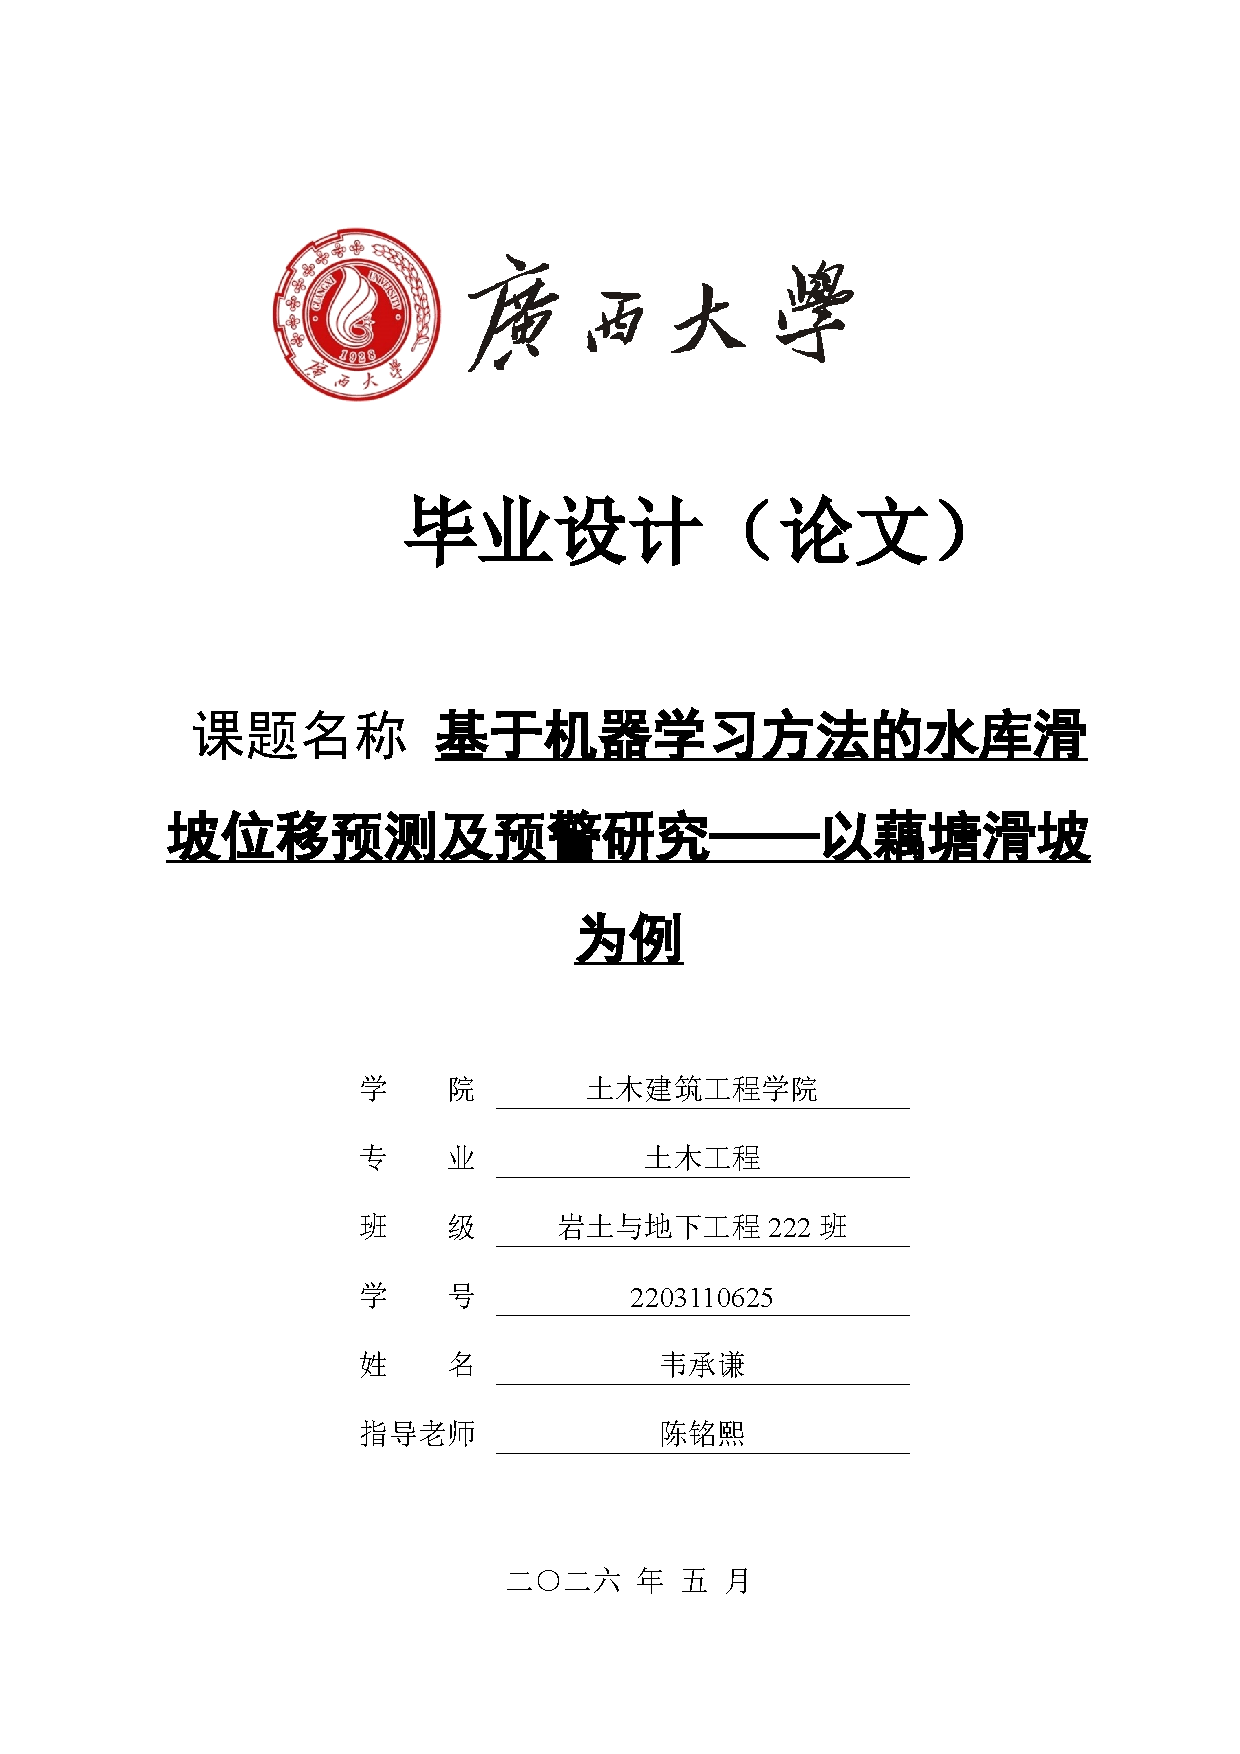
\includepdf{thesis_cover_page.pdf}


% ===== 前置部分：小写罗马数字页码 =====
\pagenumbering{roman}
\setcounter{page}{1}

% ===== 中文摘要页 =====
\addcontentsline{toc}{section}{摘要}
\thispagestyle{plain}
\begin{center}
  {\setstretch{1.25}\fontsize{16pt}{20pt}\selectfont\heiti\bfseries
  基于机器学习方法的水库滑坡位移预测及预警研究——以藕塘滑坡为例}
\end{center}

\vspace{\baselineskip}

\begin{center}
  {\fontsize{16pt}{20pt}\selectfont\heiti\bfseries 摘\hspace{0.6em}要}
\end{center}

\vspace{\baselineskip}

{\fontsize{12pt}{14.5pt}\selectfont\songti\rmfamily
三峡库区水库滑坡受库水位周期性涨落与季节性降雨的耦合驱动，呈现出典型的阶跃型变形特征。本文以三峡库区典型阶跃型滑坡——藕塘滑坡为研究对象，构建了一套“特征分析—位移预测—概率预警”的机器学习研究框架。

首先，采用LightGBM结合SHAP可解释性方法，对多源监测数据进行特征重要性分析，定性揭示历史位移累积与库水位滞后特征是滑坡位移预测的主控因子，降雨、地下水位次之，气象特征（温度、露点、湿度）贡献最小。

其次，基于多监测点空间运动学输入，构建了长短期记忆网络（LSTM）时序预测模型，对MJ9、MJ1、MJ3三个代表性监测点分别进行50次独立随机初始化训练。测试集结果表明，LSTM模型在MJ1点取得了典型的预测性能：平均$R^2=0.7916$、平均RMSE$=$5.55~mm、相对误差约0.56\%；MJ9与MJ3两点的相对误差分别约为2.9\%与1.0\%，均处于工程可接受区间。

最后，基于匀速变形段的位移速率统计$V_0 = 1.5\bar V + 2\sigma$，构建了由各监测点自身位移本底确定阈值的四级动态预警体系（绿/黄/橙/红）；将LSTM 50次独立训练的预测月速率分布映射到4个等级区间，直接统计概率并取最高者为当日预警等级。在藕塘滑坡的验证中，测试集盲测下本方法在三点均保持100\%的特异性、零误报；训练期2017年阶跃段in-sample演示中MJ1与MJ3分别触发70天与129天黄色预警，验证了方法对阶跃变形事件的响应能力。
}

\vspace{\baselineskip}

{\fontsize{12pt}{14.5pt}\selectfont\rmfamily
\noindent\hspace{2em}{\heiti\bfseries 关键词}{\songti ：水库滑坡\hspace{1.2em}位移预测\hspace{1.2em}机器学习\hspace{1.2em}LSTM\hspace{1.2em}预警}
}

\newpage

% ===== 英文摘要页 =====
\addcontentsline{toc}{section}{ABSTRACT}
\thispagestyle{plain}

% 题目首字母及实词首字母大写，居中，Times New Roman 三号
\begin{center}
  {\setstretch{1.25}\fontsize{16pt}{20pt}\selectfont\rmfamily\bfseries
  Research on Reservoir Landslide Displacement Prediction and Early Warning Based on Machine Learning Methods}
\end{center}

\vspace{\baselineskip}

\begin{center}
  {\fontsize{16pt}{20pt}\selectfont\rmfamily\bfseries ABSTRACT}
\end{center}

\vspace{\baselineskip}

% 摘要正文，小四号(12pt)，每段开头2字符空格，Times New Roman
{\fontsize{12pt}{14.5pt}\selectfont\rmfamily
\noindent\hspace{2em}Reservoir landslides in the Three Gorges Reservoir area, driven by the coupled effects of periodic water level fluctuations and seasonal rainfall, exhibit typical step-like deformation. Taking the Outang landslide as the subject, this study builds a machine learning framework of ``feature analysis---displacement prediction---probabilistic early warning''.

\noindent\hspace{2em}First, LightGBM combined with SHAP is applied to multi-source monitoring data, qualitatively identifying historical displacement accumulation and lagged reservoir water level as dominant drivers, followed by rainfall and groundwater level, while meteorological variables contribute the least.

\noindent\hspace{2em}Second, an LSTM time-series model is trained 50 times independently on MJ9, MJ1 and MJ3. At MJ1, the model achieves a mean $R^2 = 0.7916$ and RMSE of 5.55~mm (relative error 0.56\%); MJ9 and MJ3 remain within engineering-acceptable relative errors of approximately 2.9\% and 1.0\%.

\noindent\hspace{2em}Finally, a four-level dynamic warning system (green/yellow/orange/red) is built upon a per-point reference velocity $V_0 = 1.5\bar V + 2\sigma$ from the steady-state stage. The 50 LSTM predictions yield a monthly-velocity distribution whose empirical probabilities over the four intervals drive level selection. In validation, the out-of-sample test exhibits 100\% specificity with zero false alarms at all three points; during the 2017 step-deformation in-sample demonstration, MJ1 and MJ3 trigger 70 and 129 days of yellow warning respectively, confirming the method's responsiveness to real step events.
}

% 摘要正文与KEYWORDS之间空一行
\vspace{\baselineskip}

{\fontsize{12pt}{14.5pt}\selectfont\rmfamily
\noindent\textbf{Keywords}: Reservoir Landslide; Displacement Prediction; Machine Learning; LSTM; Early Warning
}

\newpage

% 目录标题局部覆盖为三号(16pt)黑体居中，上下空一行
\begingroup
  \titleformat{\section}[block]
    {\centering\fontsize{16pt}{20pt}\selectfont\heiti\bfseries}
    {}{0em}{}
  \titlespacing*{\section}{0pt}{\baselineskip}{\baselineskip}
  \tableofcontents
\endgroup

\newpage

% ===== 正文：阿拉伯数字页码从1开始 =====
\pagenumbering{arabic}
\setcounter{page}{1}

\section{绪论}

\subsection{研究意义和目的}

\subsubsection{理论意义}

本研究针对大型水库滑坡内部变形空间不均匀及多场耦合机制复杂的科学难题，旨在突破传统单点位移预测模型割裂滑坡体时空联系的局限性。三峡库区特大型滑坡（如藕塘滑坡）通常具有显著的分区、分级变形特征，传统的时间序列分析方法往往难以揭示滑坡后缘推力与前缘阻滑效应之间的力学传递规律。本课题通过构建基于时空图神经网络的预测架构，将滑坡视为一个有机互馈的动力学系统，有助于从数据驱动的视角厘清滑坡不同块体间的协同演化机制与链式响应规律，为完善复杂岩土介质的非线性动力学理论提供新的切入点。此外，针对深度学习模型普遍存在的“黑箱”问题，本研究引入特征归因分析方法，致力于定量解析库水位涨落与降雨入渗对滑坡位移的“滞后衰减效应”及贡献权重。这种尝试不仅赋予了机器学习模型以明确的物理可解释性，也为揭示“水-土”相互作用下阶跃型滑坡的成因机理提供了可量化的数据支撑，实现了从纯粹的数据挖掘向地质机理反演的理论跨越。

\subsubsection{现实意义}

本课题的研究成果对于提升三峡库区重大地质灾害的防灾减灾水平具有重要的应用价值。藕塘滑坡作为三峡库区体积巨大、变形机制复杂的典型涉水滑坡，其稳定性直接关系到长江黄金水道的通航安全及库区沿岸居民的生命财产安全。本研究构建的高精度时空位移预测模型，旨在解决传统方法在极端水文气象工况（如库水位急剧下降叠加持续强降雨）下预测精度失效的难题，力争实现对滑坡灾变趋势的毫米级精准把控。更为关键的是，本研究不再满足于单一的位移数值预报，而是建立基于置信区间的动态概率预警体系。这将为地质灾害防治部门提供包含风险概率的科学决策依据，有效降低因监测噪声或局部扰动导致的误报率与漏报率。通过显著延长有效预警的时间窗口，本研究可为制定库水位应急调度方案、实施航道交通管制以及组织人员避险转移争取宝贵的“黄金时间”，从而最大限度地降低潜在的灾害风险与社会经济损失。

\subsubsection{目的}

本研究旨在通过运用岩土工程与计算机科学交叉学科知识，巩固深化岩土力学、边坡工程及机器学习算法的基本理论，学习和理解滑坡演化机理及预测预警的前沿方法。具体目标包括：

    （1）通过查阅国内外文献，系统掌握机器学习在滑坡位移预测中的原理和方法，梳理该领域的研究现状与发展趋势；

    （2）选取三峡库区典型阶跃型滑坡——藕塘滑坡为研究对象，深入分析滑坡累积位移与库水位周期性涨落、季节性降雨等外部诱发因子之间的非线性关系及滞后规律；

    （3）基于Python环境（PyTorch框架）构建机器学习预测模型，通过数据处理、特征工程、模型构建及结果分析的全过程训练，掌握数据驱动的滑坡位移预测方法与步骤；

    （4）基于多次独立训练构建滑坡位移的概率预测区间，制定科学的滑坡分级预警判据，为防灾减灾提供决策依据；

    （5）通过建立机器学习预测模型的全过程训练，获得科研工作的基本训练，提高分析复杂岩土工程问题和解决问题的能力。

\subsection{滑坡位移预测研究现状}


\subsubsection{国外研究动态}

国外在滑坡灾害预测与预警领域的研究起步较早，近年来，该领域正经历着从单一物理模型向“数据-物理”深度融合的范式转变。最新的国际研究趋势不再局限于对监测数据的简单数值拟合，而是更加强调机器学习模型在复杂地质环境下的物理一致性与泛化能力。特别是在物理信息机器学习（PIML）领域，研究重心已显著转向将非饱和土力学中的控制方程或边坡稳定性物理约束直接嵌入神经网络的损失函数中，以解决小样本条件下的“黑箱”不可靠难题。

在监测技术与空间协同预警方面，构建大范围区域的滑坡灾害时空动态感知系统已成为主流。最新的国际学术期刊研究显示，利用合成孔径雷达干涉测量（InSAR）技术获取地表形变场，并结合深度学习算法构建区域滑坡动态评估框架是当前的热点。例如，Zhang等\cite{zhang2025spatiotemporal}提出了一种融合空间图神经网络（GCN）与时间卷积网络（TCN）的时空位移预测模型（GMTC）。该研究利用Sentinel-1A卫星数据对滑坡进行三维形变分解，并通过多头自注意力机制捕捉滑坡形变在时空维度的非线性动态特征，显著优于传统的GRU和GCN模型，实现了对滑坡位移的高精度预测。

在位移预测模型方面，Guo等\cite{guo2020landslide}较早将变分模态分解与灰狼优化算法及BP神经网络相结合，建立了WA-GWO-BP混合预测模型，验证了信号分解与机器学习融合策略在滑坡位移预测中的有效性。Wang等\cite{wang2025enhancing}进一步提出了融合时空深度学习与可解释特征的滑坡位移预测框架，通过时空图模型同时捕捉滑坡变形的空间相关性与时序依赖性，并引入特征归因分析增强模型透明度。

此外，针对人工智能在防灾减灾决策中的信任问题，可解释性人工智能（Explainable AI, XAI）已成为当前国际滑坡研究的重要方向。为了将复杂的机器学习预测结果转化为决策者可理解的预警信息，国际学者引入了SHAP（Shapley Additive explanations）等归因分析方法。例如，Al-Najjar等\cite{al2025shapley}针对滑坡易发性建模中的“黑箱”问题，利用SHAP方法对随机森林模型的预测结果进行了全方位的解释。该研究不仅量化了地质环境因子（如地形、地质构造等）对模型预测的非线性贡献度，还通过可视化手段展示了特征交互作用，为制定科学的风险管控策略提供了强有力的理论依据，有效弥合了复杂算法与实际防灾应用之间的鸿沟。

\subsubsection{国内研究动态}

中国作为世界上水库滑坡灾害最为频发的国家之一，特别是三峡库区，其特殊的地质环境与周期性的库水位涨落（145米至175米）叠加季节性强降雨，使得滑坡演化机制极为复杂。针对水库滑坡特有的“阶梯状”演化特征，国内学术界已经建立了一套相对成熟的“时序分解-多源重构-组合预测”研究范式。早期的研究主要致力于解决非线性位移数据的降噪与分量提取问题，广泛采用了变分模态分解（VMD）、改进自适应噪声完备集合经验模态分解（ICEEMDAN）等信号处理技术。例如，马佳伟等\cite{ma2025iceemdan}建立了一种基于ICEEMDAN-CNN-BiLSTM-XGBoost的双层融合预测模型，有效解决了传统模型在位移分解中存在的模态混叠问题。在此基础上，国内学者通过引入智能优化策略，构建混合预测模型。唐宇峰等\cite{tang2025pso}提出的PSO-GRU-OL-MRT模型，通过深度挖掘位移监测数据与诱发因子之间的高维非线性映射关系，显著提升了滑坡位移的实时预测精度。姜宇航等\cite{jiang2022pso}将粒子群优化算法与VMD及NARNN-GRU相结合，构建了PSO-VMD-NARNN-GRU滑坡位移动态预测模型，有效提升了非线性位移序列的分解质量与预测精度。刘艺梁等\cite{liu2026vmd}针对库岸滑坡位移预测中的时滞效应问题，提出了基于VMD-SSA-LSSVM的预测方法，利用麻雀搜索算法（SSA）优化最小二乘支持向量机参数，在考虑时滞效应的基础上实现了更高的预测精度。王东民等\cite{wang2025optimization}进一步从优化时序分解与特征选择的角度出发，构建了融合多策略的滑坡位移预测模型，系统提升了输入特征的质量与模型的泛化性能。

随着人工智能技术的迭代升级，国内研究重点正逐步从传统的递归神经网络向基于注意力机制（Attention Mechanism）和Transformer架构的第三代深度学习模型演进。针对传统模型难以量化降雨和库水位“滞后效应”的痛点，最新的研究工作通过在模型中嵌入自注意力模块，实现了对多源诱发因子长时序依赖关系的动态捕捉。汪松林等\cite{wang2025transformer}构建了基于特征增强的Transformer-GRU模型，该模型不仅能够自动识别不同变形阶段的关键驱动因子，还能通过可视化权重分配，从数据层面反演滑坡对水文气象条件的响应规律。与此同时，针对特大型涉水滑坡（如藕塘滑坡）往往存在多级滑体且各部位变形不同步的特征，国内学者开始探索基于时空协同的预测新模式。高振武等\cite{gao2025spatiotemporal}提出了一种基于多测点时空模态信息互馈的阶跃式滑坡位移预测方法，通过融合多测点的时空模态信息，有效解决了局部监测噪声干扰导致的误报问题。

针对时滞效应的量化问题，杜岩等\cite{du2024time}系统研究了考虑时间滞后效应的库岸滑坡位移预测方法，基于自回归分布滞后（ARDL）模型建立了库岸滑坡位移预测模型，工程案例得出库水位作用于滑坡变形的滞后天数为8天。凌晴等\cite{ling2025lag}提出了基于滞后衰减效应与主控因子筛选策略的库岸滑坡位移预测模型，通过构建滞后衰减系数定量刻画了诱发因子随时间衰减的影响规律，并结合主控因子筛选有效降低了输入特征冗余。

在模型多样性方面，秦世伟等\cite{qin2025cnn}构建了基于多变量CNN-LSTM神经网络的滑坡位移预测模型，充分利用CNN的空间特征提取能力与LSTM的时序建模能力。陈朗等\cite{chen2024gaussian}、吴成杰等\cite{wu2026gaussian}分别从前期累积降雨与多源时序特征融合的角度，引入高斯过程回归（GPR）模型，不仅提供了位移的点预测值，还输出了预测方差，为滑坡位移的不确定性量化提供了新思路。冯谕等\cite{feng2025creep}则从蠕滑趋势影响的角度出发，结合特征优化算法构建了针对阶跃型滑坡的位移预测模型，有效增强了模型对蠕滑变形阶段的识别能力。

在区域尺度滑坡监测与预测方面，林满生\cite{lin2025improved}基于改进卷积神经网络开展了滑坡空间预测与边坡稳定性评估研究，验证了深度学习方法在区域滑坡易发性建模中的适用性。谭力兵\cite{tan2025insar}将时序InSAR技术与深度学习方法相结合，开展了库岸滑坡形变的时空分析与预测，为融合天基遥感观测与地面监测数据的滑坡预测提供了新途径。



\subsection{滑坡预警研究现状}

在预警决策与风险评估方面，国内外研究正在推动从确定性的“点预测”向不确定性的“概率区间预测”跨越，旨在解决单纯数值预测无法量化风险可信度的问题。鉴于滑坡系统的随机性与模糊性，部分前沿学者将核密度估计（KDE）理论与深度学习预测结果相结合，构建了包含置信区间的概率预测模型，实现了对位移波动范围的科学度量。例如，王石等\cite{wang2025ssa}提出了基于SSA-CNN-BiLSTM-AM和KDE的滑坡位移混合点-区间预测方法，该方法不仅提供了位移的点预测值，还通过KDE方法构建了预测区间，量化了预测结果的不确定性，为滑坡预警提供了更加可靠的决策依据。

更为深入的研究则进一步将位移预测延伸至物理力学层面的稳定性评估，提出了考虑滑带土应变软化特性的时变失效概率分析方法。通过建立滑坡稳定系数与库水位变动、降雨入渗及累积变形之间的动态响应方程，研究人员实现了对滑坡全生命周期灾变风险的动态追踪。孟轩宇\cite{meng2024time}针对三峡库区阶跃型库岸滑坡，提出了时变失效概率预测方法，该方法综合考虑了库水位涨落、降雨入渗以及滑带土应变软化等多重因素对滑坡稳定性的影响，实现了对滑坡灾变风险的定量评估。Zou等\cite{zou2023novel}以藕塘滑坡为例，提出了一种评估水库滑坡时变稳定性的新方法，该方法通过建立滑坡稳定系数与环境因子之间的动态响应模型，实现了对滑坡稳定性的实时监测与预警。

这种融合了“数据驱动的高精度预测”与“物理驱动的稳定性评价”的综合研究体系，标志着国内外水库滑坡防灾减灾技术正朝着精细化、智能化和实用化的方向迈进。通过将机器学习的强大预测能力与岩土工程的物理机理相结合，不仅提高了滑坡位移预测的精度，还增强了预警系统的可靠性和可解释性，为地质灾害防治部门提供了更加科学、全面的决策支持。




\subsection{主要研究内容及技术路线}

\subsubsection{主要研究内容}

本研究以三峡库区典型阶跃型滑坡——藕塘滑坡为研究对象，围绕机器学习方法在水库滑坡位移预测及预警中的应用展开系统研究。主要研究内容包括以下三个方面：

\paragraph{（1）滑坡变形演化机理与多源特征工程构建}

深入分析藕塘滑坡累积位移与库水位周期性涨落、季节性降雨等外部诱发因子之间的非线性关系及滞后规律。对长序列监测数据进行清洗、降噪及归一化处理，利用可解析性机器学习方法（如LightGBM+SHAP）筛选出主控影响因子，定量评估各触发因子对滑坡位移的贡献度。通过特征重要性分析、局部依赖图和特征交互效应图等多维度可视化手段，揭示水文气象因素与滑坡变形之间的内在非线性映射关系，完成多源特征工程的构建，为模型训练提供高质量的输入数据。

\paragraph{（2）基于机器学习的滑坡位移预测模型搭建}

基于Python环境（PyTorch框架）搭建机器学习预测模型。针对滑坡变形的时空演化特征，利用LSTM网络捕捉多源数据融合与长时序依赖关系，对藕塘滑坡多个代表性监测点进行50次独立随机初始化训练，以$R^2$与RMSE为主要精度指标评估模型在训练集与测试集上的表现与稳定性，重点关注阶跃变形期的预测效果。

\paragraph{（3）基于$V_0$阈值的概率预警方法研究}

针对传统固定阈值在不同监测点间缺乏可比性、确定性点预测难以反映结果可信度的问题，提出由监测数据内生确定阈值的四级（绿/黄/橙/红）动态预警体系。具体通过对各监测点匀速变形阶段的位移速率统计量$V_0 = 1.5\bar V + 2\sigma$及其倍数递进阈值（$V_0/5V_0/10V_0$）划定预警等级区间；并将第三章LSTM 50次独立训练得到的预测月速率分布映射到4个等级区间，直接统计各等级概率，取最高概率等级作为当日预警结果，实现从单点确定性预报向分布式概率预警的转变，为防灾减灾提供决策依据。

\subsubsection{拟解决的主要问题}

本研究针对水库滑坡位移预测与预警中的关键科学问题，拟重点解决以下三个方面的难题：

\paragraph{（1）多源诱发因子的“最佳时滞”特征优选问题}

库水位和降雨对滑坡的影响具有显著的滞后性与非线性特征。拟解决如何从海量监测数据中，精准识别出降雨和库水位影响滑坡变形的最优滞后时间窗口。通过有效的特征选择与降维策略，剔除冗余特征干扰，提高模型输入变量的物理相关性与有效性，解决多源数据输入的高维冗余难题。

\paragraph{（2）阶跃型滑坡“突变点”的预测削峰与滞后问题}

常规机器学习模型在滑坡位移加速变形期（阶跃点）容易出现“削峰”现象（预测值偏低）或相位滞后，难以捕捉极端工况下的突变特征。拟解决如何通过改进模型架构或引入特征增强策略，提升模型对暴雨、水位急降等强激发条件下位移非线性动态变化的敏感性，进而提高阶跃变形期的峰值预测精度。

\paragraph{（3）预测结果的不确定性量化与预警可靠性问题}

传统确定性点预测无法反映预测结果的可信度。拟解决如何构建包含置信度的概率预测区间，量化模型的不确定性风险，为滑坡预警提供更科学的决策依据。通过建立基于概率区间的动态预警体系，有效降低因监测噪声或局部扰动导致的误报率与漏报率。

\subsubsection{技术路线}

本研究的技术路线围绕“特征提取—位移预测—概率预警”三个递进环节展开，具体如下：

\paragraph{一、数据收集与预处理}

    （1）收集藕塘滑坡长时间序列监测数据，包括地表位移（MJ9、MJ1、MJ3等监测点）、库水位、日降雨量、地下水位及气象要素（温度、湿度、露点）；

    （2）对原始数据进行清洗、缺失值插补与归一化处理，采用滑动时间窗口（5天）构建监督学习样本集；

    （3）基于先验地质知识，初步筛选具有物理意义的候选特征，构建包含历史位移、水文气象滞后特征及监测点标识的多源候选特征集。

\paragraph{二、可解释机器学习特征分析}

    （1）以LightGBM为基础模型，分别构建位移增量回归模型与预警状态分类模型，采用5折时序交叉验证评估模型性能，并引入SMOTE过采样技术处理类别不平衡问题；

    （2）引入SHAP（Shapley Additive Explanations）方法对模型进行可解释性分析，通过特征贡献图、依赖图和交互图，定量揭示库水位、降雨、地下水位等触发因子对滑坡位移的贡献度、非线性响应规律及耦合效应；

    （3）基于SHAP分析结果，筛选主控特征，为后续预测模型提供高质量输入变量，并从数据层面验证滑坡变形的多因子累积驱动机制假设。

\paragraph{三、基于LSTM的多监测点位移预测}

    （1）以多监测点历史累积位移序列作为空间运动学输入特征，构建LSTM时序预测模型，利用滑坡体的空间协同变形信息提升目标监测点的位移预测精度；

    （2）对MJ9、MJ1、MJ3三个代表性监测点分别进行50次独立随机初始化训练，收集预测结果的统计分布；

    （3）以$R^2$与RMSE（50次独立运行的逐次算术平均）评估各点点预测精度与稳定性，并结合相对误差进行工程意义上的综合评价。

\paragraph{四、基于$V_0$阈值的四级动态预警体系}

    （1）对各监测点匀速变形阶段的位移速率序列，按$V_0 = 1.5\bar V + 2\sigma$确定基准速率，并按$V_0/5V_0/10V_0$递进设定绿/黄/橙/红四级阈值；

    （2）将50次独立LSTM预测得到的月速率分布映射到四个等级区间，直接统计每一天四级预警的发生概率，并取概率最高者作为当日预警等级；

    （3）以测试集盲测下的特异性、误报率以及训练期阶跃段的黄色预警触发情况综合评估预警体系，分析方法在误报控制与阶跃响应两方面的表现。

\begin{figure}[H]
\centering
\scalebox{0.85}{%
\begin{tikzpicture}[
    node distance=0cm,
    every node/.style={font=\small},
    titlebox/.style={rectangle, draw=black, fill=blue!25, rounded corners=4pt,
                     text centered, minimum width=10cm, minimum height=0.7cm,
                     font=\small\bfseries, text width=9.5cm, inner sep=4pt},
    phasebox/.style={rectangle, draw=black!80, fill=blue!12, rounded corners=3pt,
                     text centered, minimum width=10cm, minimum height=0.65cm,
                     font=\small\bfseries, text width=9.5cm, inner sep=4pt},
    stepbox/.style={rectangle, draw=black!40, fill=gray!8, rounded corners=2pt,
                    text centered, minimum width=9cm, minimum height=0.55cm,
                    font=\small, text width=8.5cm, inner sep=3pt},
    resultbox/.style={rectangle, draw=black, fill=green!20, rounded corners=4pt,
                      text centered, minimum width=10cm, minimum height=0.7cm,
                      font=\small\bfseries, text width=9.5cm, inner sep=4pt},
    arr/.style={->, >=stealth, thick, draw=black!60},
]

\node[titlebox] (goal) {基于机器学习的滑坡位移预测与概率预警};

\node[phasebox, below=0.5cm of goal]  (p1)  {第一阶段：数据收集与预处理};
\node[stepbox,  below=0.2cm of p1]   (s11) {收集地表位移、库水位、降雨量等长时序监测数据};
\node[stepbox,  below=0.15cm of s11] (s12) {数据清洗、缺失值插补与归一化处理};
\node[stepbox,  below=0.15cm of s12] (s13) {滑动时间窗口构建监督学习样本集，初步筛选候选特征};

\node[phasebox, below=0.5cm of s13]  (p2)  {第二阶段：可解释机器学习特征分析};
\node[stepbox,  below=0.2cm of p2]   (s21) {LightGBM模型训练与5折时序交叉验证};
\node[stepbox,  below=0.15cm of s21] (s22) {SHAP可解释性分析（贡献图、依赖图、交互图）};
\node[stepbox,  below=0.15cm of s22] (s23) {主控特征筛选，验证历史位移累积与库水位滞后的主控作用};

\node[phasebox, below=0.5cm of s23]  (p3)  {第三阶段：LSTM多监测点位移预测};
\node[stepbox,  below=0.2cm of p3]   (s31) {多监测点空间运动学输入，构建LSTM时序预测模型};
\node[stepbox,  below=0.15cm of s31] (s32) {三点各自50次独立随机初始化训练};
\node[stepbox,  below=0.15cm of s32] (s33) {$R^2$与RMSE逐次均值评估点预测精度与稳定性};

\node[phasebox, below=0.5cm of s33]  (p4)  {第四阶段：$V_0$阈值四级动态预警体系};
\node[stepbox,  below=0.2cm of p4]   (s41) {$V_0=1.5\bar V+2\sigma$ 及 $V_0/5V_0/10V_0$ 递进阈值分级};
\node[stepbox,  below=0.15cm of s41] (s42) {50次预测月速率分布映射到四级概率，取最高概率等级};

\node[resultbox, below=0.5cm of s42] (res) {高精度位移预测模型与可靠概率预警体系};

\draw[arr] (goal) -- (p1);
\draw[arr] (p1)   -- (s11);
\draw[arr] (s11)  -- (s12);
\draw[arr] (s12)  -- (s13);
\draw[arr] (s13)  -- (p2);
\draw[arr] (p2)   -- (s21);
\draw[arr] (s21)  -- (s22);
\draw[arr] (s22)  -- (s23);
\draw[arr] (s23)  -- (p3);
\draw[arr] (p3)   -- (s31);
\draw[arr] (s31)  -- (s32);
\draw[arr] (s32)  -- (s33);
\draw[arr] (s33)  -- (p4);
\draw[arr] (p4)   -- (s41);
\draw[arr] (s41)  -- (s42);
\draw[arr] (s42)  -- (res);

\end{tikzpicture}%
}
\figcaption{技术路线图}{Technical Roadmap}
\label{fig:tech_roadmap}
\end{figure}


\section{基于可解释机器学习的滑坡位移特征提取与贡献度分析}

\subsection{前言}

在构建数据驱动的水库滑坡时空位移预测模型时，输入特征的科学选取直接决定了模型的预测精度与泛化能力。传统基于经验的特征选择方法虽具备一定的工程地质学基础，但在处理复杂非线性的监测数据时往往带有较强的主观性，难以定量刻画各诱发因素的具体影响程度，缺乏统一的标准。为此，本章引入高效的梯度提升框架（LightGBM）与可解释性机器学习工具（SHAP），旨在对滑坡变形的候选驱动因子进行精准的定量评估与优选。本研究以典型的藕塘滑坡为案例，针对其复杂的地质演化特征，收集并整理了该区域长时间序列的库水位、降雨量及地表时空位移等监测数据。基于LightGBM模型的高效拟合能力，结合SHAP方法深入剖析各输入特征对滑坡时空位移的贡献度。通过特征重要性图、局部依赖图和特征交互效应图等多维度的可视化分析，系统揭示水文气象因素与滑坡变形之间的内在非线性映射关系。本章采用“先验知识指导初筛+数据算法量化验证”的研究策略，不仅有效克服了传统机器学习模型“黑盒”特性的不足，提升了特征选择的科学性与物理可解释性，更为后续构建高精度的藕塘滑坡时空位移预测及预警模型奠定了坚实的数据基础与理论支撑。

\begin{figure}[H]
    \centering
    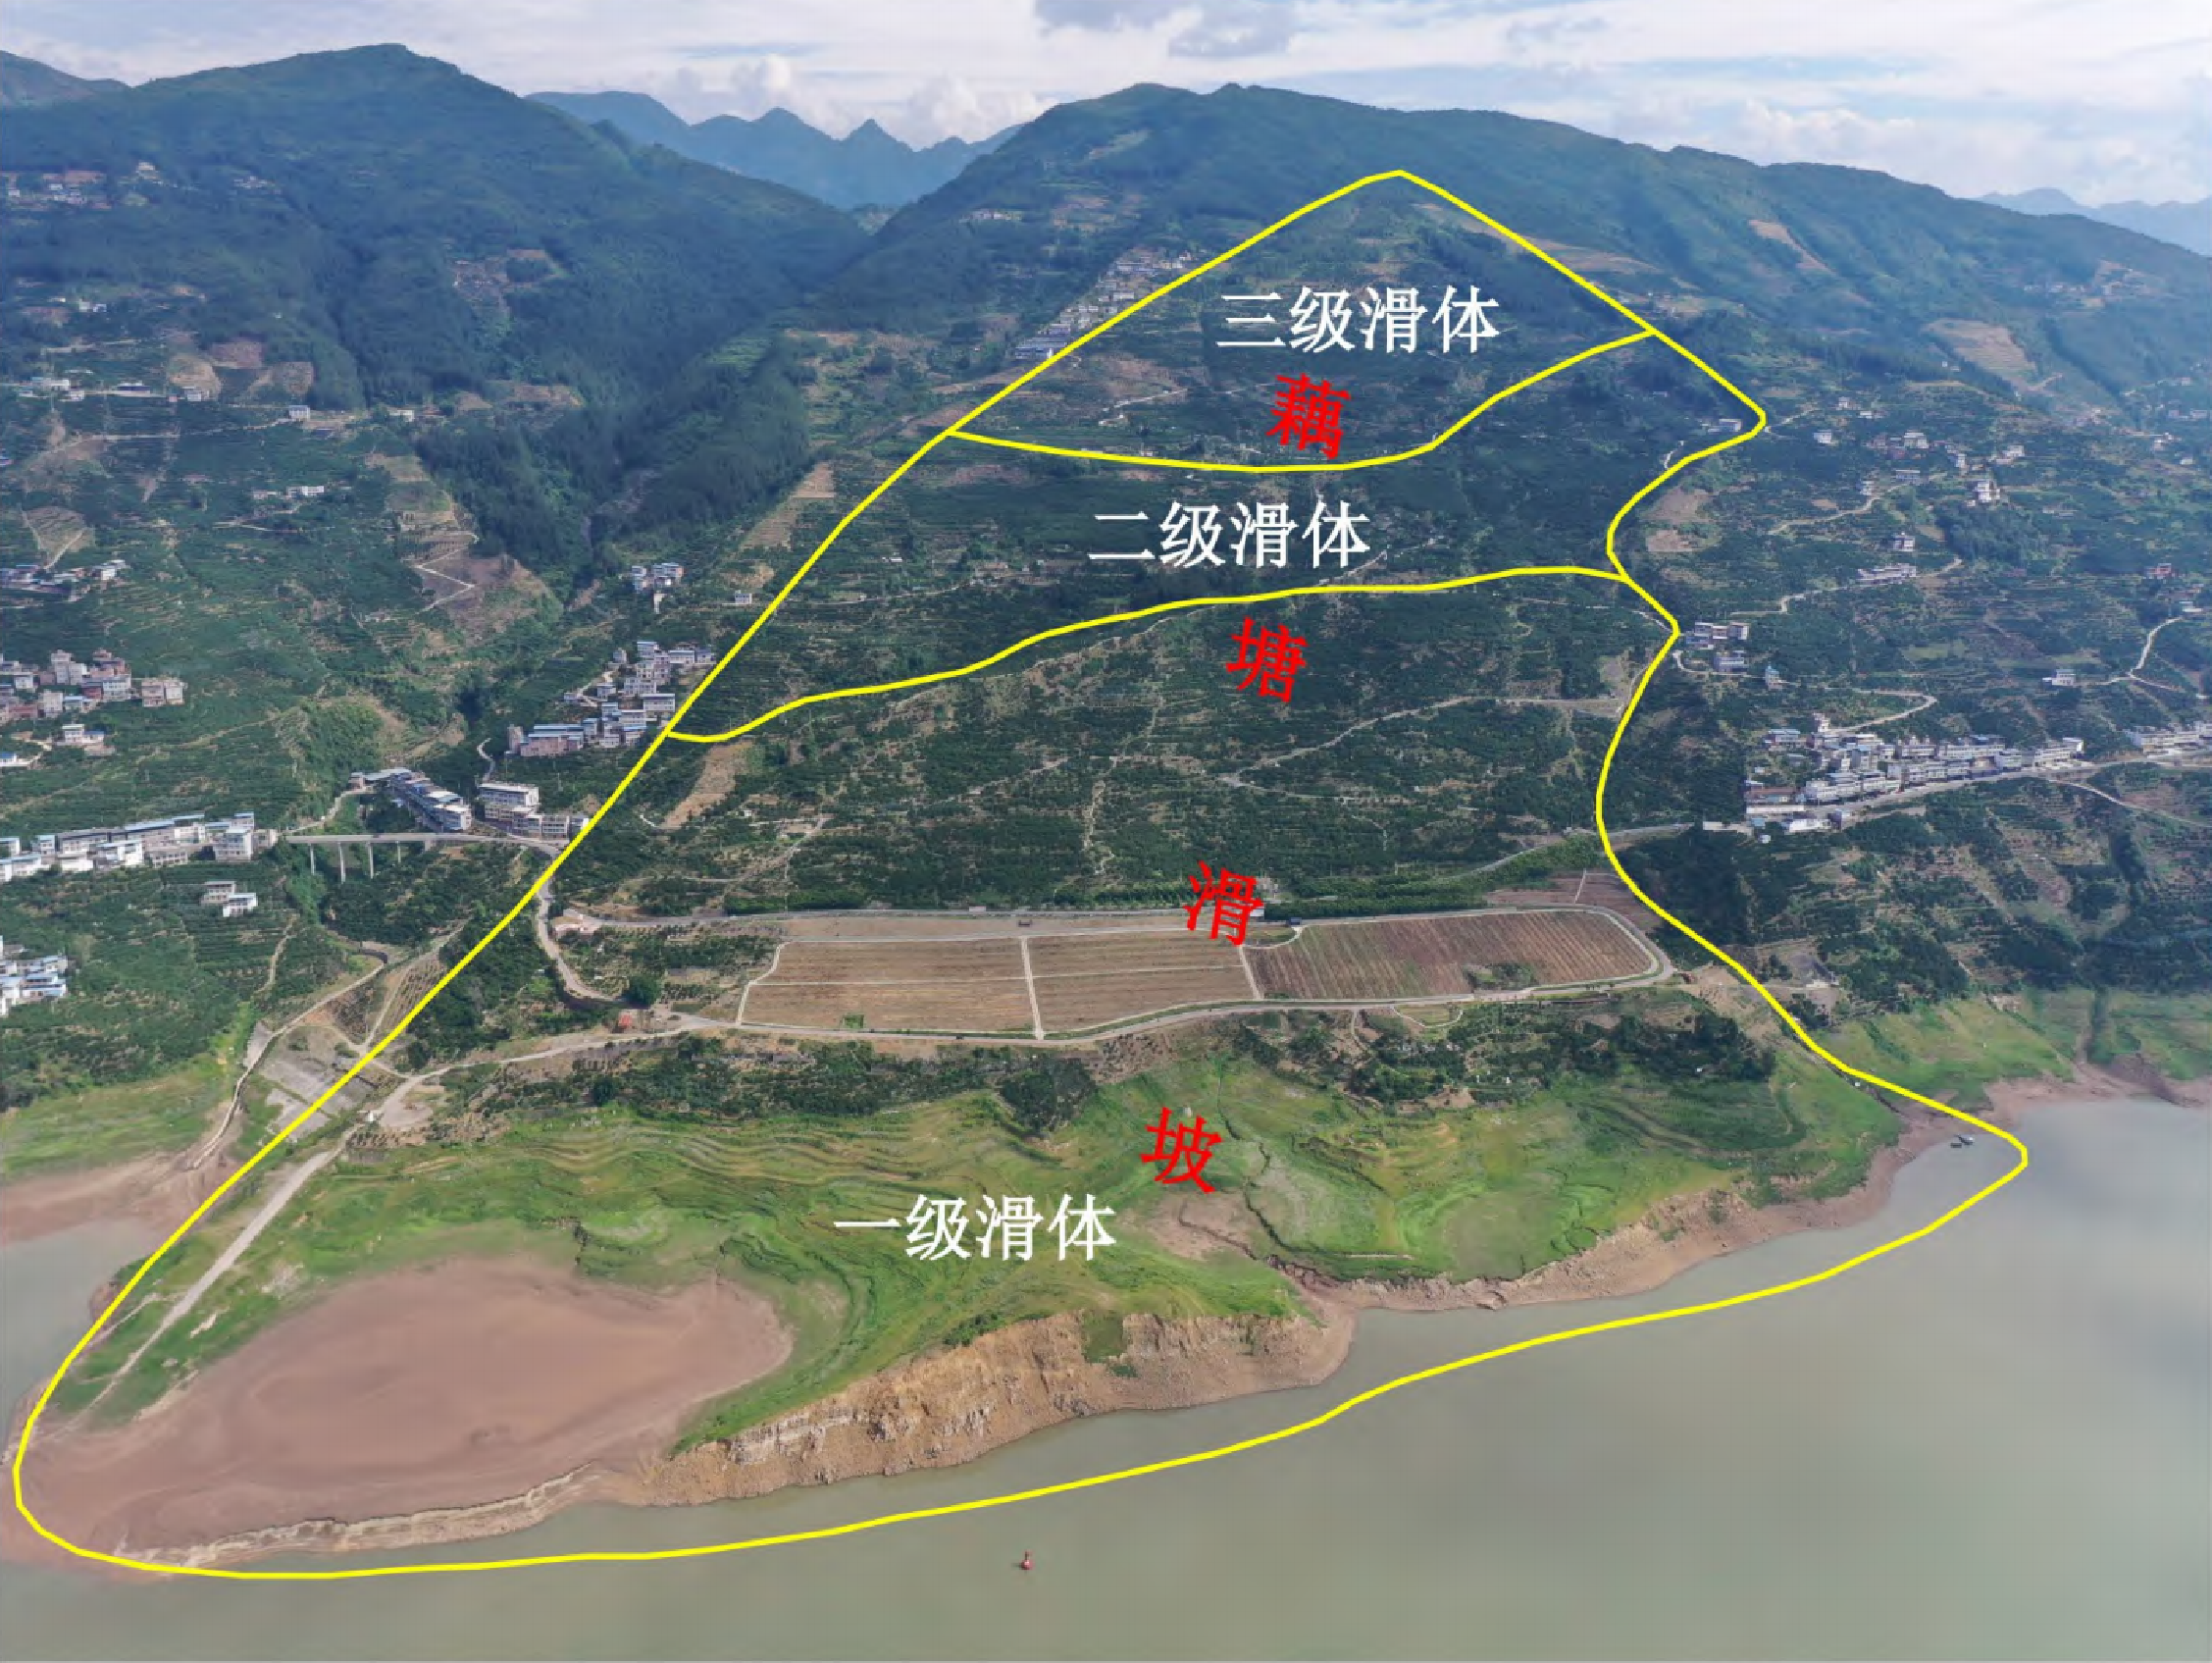
\includegraphics[width=0.83\textwidth]{figures/chapter2/Panoramic_map_of_Outang_landslide.pdf}
    \figcaption{藕塘滑坡全景图（赵长军等，2025）\cite{zhao2025reactivation}}{Panoramic View of Outang Landslide (Zhao et al., 2025)}
    \label{fig:panorama}
\end{figure}

\subsection{工程概况}

\paragraph{（1）地理位置与地形地貌}

藕塘滑坡位于三峡库区重庆市奉节县安坪镇的长江南岸，地理坐标约为东经109°22′、北纬30°57′，属于构造剥蚀的中低山河谷地貌。该区域地形总体呈南高北低之势，滑坡体后缘高程达700余米，前缘直抵长江干流，整体坡度多在15°至30°之间，局部陡坡可达35°以上。滑坡区地貌受长江及其支流的长期侵蚀切割，形成了典型的“V”形河谷地貌，坡体前缘受江水侵蚀，坡脚支撑条件较差，为滑坡的孕育和复活提供了有利的地形条件\cite{zhao2025reactivation}。受库区蓄水后水位抬升及季节性消落的影响，坡脚部位的侵蚀与掏蚀作用进一步增强，加剧了前缘阻滑段的弱化趋势。

\paragraph{（2）滑坡体基本特征}

藕塘滑坡是一处大型古滑坡复活体，总体积约为$9\times10^{7}$\,m$^{3}$，最大厚度约114\,m，平面形态呈不规则多边形\cite{huang2020deformation}。赵龙翔等\cite{zhao2022deformation}对三峡库区特大型多级岩质滑坡的变形特征进行了系统研究，揭示了此类滑坡的分区分级变形规律与多期次演化特征，为理解藕塘滑坡的变形模式提供了区域性背景参考。地质调查表明，该滑坡可划分为三个相互独立的子区，具有典型的多级多期次复合滑动特征。各子区均沿侏罗系地层中发育的软弱夹层滑动，软弱夹层主要由泥化夹层和碎裂岩带组成，其抗剪强度低、遇水软化特征显著，是控制滑坡变形的关键地质界面。自2003年三峡水库首次蓄水、2009年蓄水至175\,m正常蓄水位以来，库水位的周期性涨落打破了坡体原有的渗流平衡，导致古滑坡持续复活变形，呈现出典型的阶跃型位移特征。

\paragraph{（3）地层岩性与地质构造}

研究区出露地层主要以侏罗系（J）的泥岩、砂质泥岩与粉砂岩互层为主，岩层总体走向近东西，倾向北偏西，倾角约10°—20°，与坡面倾向基本一致，构成顺向坡结构。受区域构造作用影响，岩体中节理裂隙较为发育，为地表水的垂向入渗与地下水渗流提供了网络状通道，加速了软弱夹层中黏土矿物的泥化进程。这种软硬相间的岩层结构在长期风化和水流侵蚀下，极易沿软弱夹层形成滑动面。软弱夹层中黏粒含量高、渗透性差，在库水位波动和降雨入渗的共同作用下，孔隙水压力易于积聚，进一步降低了滑带土的抗剪强度，加剧了滑坡体的失稳趋势\cite{xiao2021outang}。

\paragraph{（4）气候与水文条件}

该地区属于亚热带季风气候，年平均气温约为18\,°C，多年平均降水量在1100\,mm左右。降水在年内分配极不均匀，主要集中在每年的5月至9月，且多以暴雨形式出现，单次强降雨事件可在短时间内引发坡体孔隙水压力的急剧升高。此外，三峡水库的周期性调度对滑坡的稳定性影响显著。库水位每年在145\,m至175\,m之间进行季节性的大幅波动：通常于9月开始蓄水，年末达到并维持175\,m高水位，次年春季逐步消落至145\,m防洪限制水位，年内水位变幅达30\,m。研究区域的地下水动态受大气降水和水库蓄水双重控制，频繁的库水位升降交替与季节性强降雨的耦合作用，不断改变着坡体的渗流场与应力状态。

\paragraph{（5）监测系统与变形特征}

为系统掌握藕塘滑坡的变形动态，相关部门在滑坡体上布设了完善的专业监测网络，主要包括GNSS地表位移监测点（MJ1、MJ3、MJ9等）、地下水位监测孔（ATU4等）以及气象监测站，实现了对滑坡地表变形、地下水动态和气象要素的全面监控\cite{li2025ps}。本研究所采用的监测数据时间跨度为2016年7月至2020年6月，共覆盖4个完整的库水位调度周期，数据集包含日尺度的地表位移、降雨量、库水位、地下水位及气象要素（温度、湿度、露点等）等多维度信息。上述多源监测数据均按日尺度连续采集，覆盖4个完整库水位调度周期的各类工况，整体数据较为系统完整，为后续章节的特征分析与模型训练提供了较为可靠的数据基础。各监测点在滑坡体上呈空间分布式布设，MJ1位于滑坡体中部、MJ3位于中后部、MJ9位于后缘，三个监测点的位移量级与变形节律存在显著差异。四年监测期内共积累有效日尺度记录1457条，涵盖了库水位从145 m至175 m的完整涨落过程及多个集中降雨时段，数据密度较高、工况覆盖较全。从监测数据来看，藕塘滑坡的位移时间序列呈现出典型的阶跃型特征：在每年库水位消落期（4—6月）与主汛期（7—9月），滑坡体发生明显的加速变形，位移增量显著；而在库水位高水位维持期（10月至次年3月），滑坡体变形趋于平缓，位移增量较小。这种“快—慢—快”的周期性变形模式与库水位调度和降雨的季节性规律高度吻合，表明库水位下降与强降雨是触发滑坡阶跃变形的主要外部诱因。不同监测点的年均位移量存在明显差异：后缘MJ9点变幅最小、中后部MJ3与中部MJ1点变幅较大，这一空间分异格局与滑坡体自后缘向前缘的渐进式推挤变形模式基本吻合，反映了滑坡体内部变形的空间不均匀性。不同监测点对库水位消落与强降雨耦合作用的响应灵敏度也存在差异，MJ1与MJ3较为敏感，MJ9响应相对滞后，为本研究开展时空位移预测提供了重要依据。

鉴于藕塘滑坡体量巨大、地质条件复杂且变形响应极其敏感，将其作为时空位移预测及预警模型研究的案例，具有重要的科学意义与防灾减灾实践价值。该滑坡所具备的分区分级变形特征、多因素耦合驱动机制及长时序监测数据积累，为验证数据驱动型滑坡预测方法的有效性提供了较为理想的研究场景。基于上述工程地质背景与监测数据基础，下文将引入LightGBM与SHAP可解释性分析方法，对滑坡位移的主控触发因子进行定量评估与优选。

\begin{figure}[H]
    \centering
    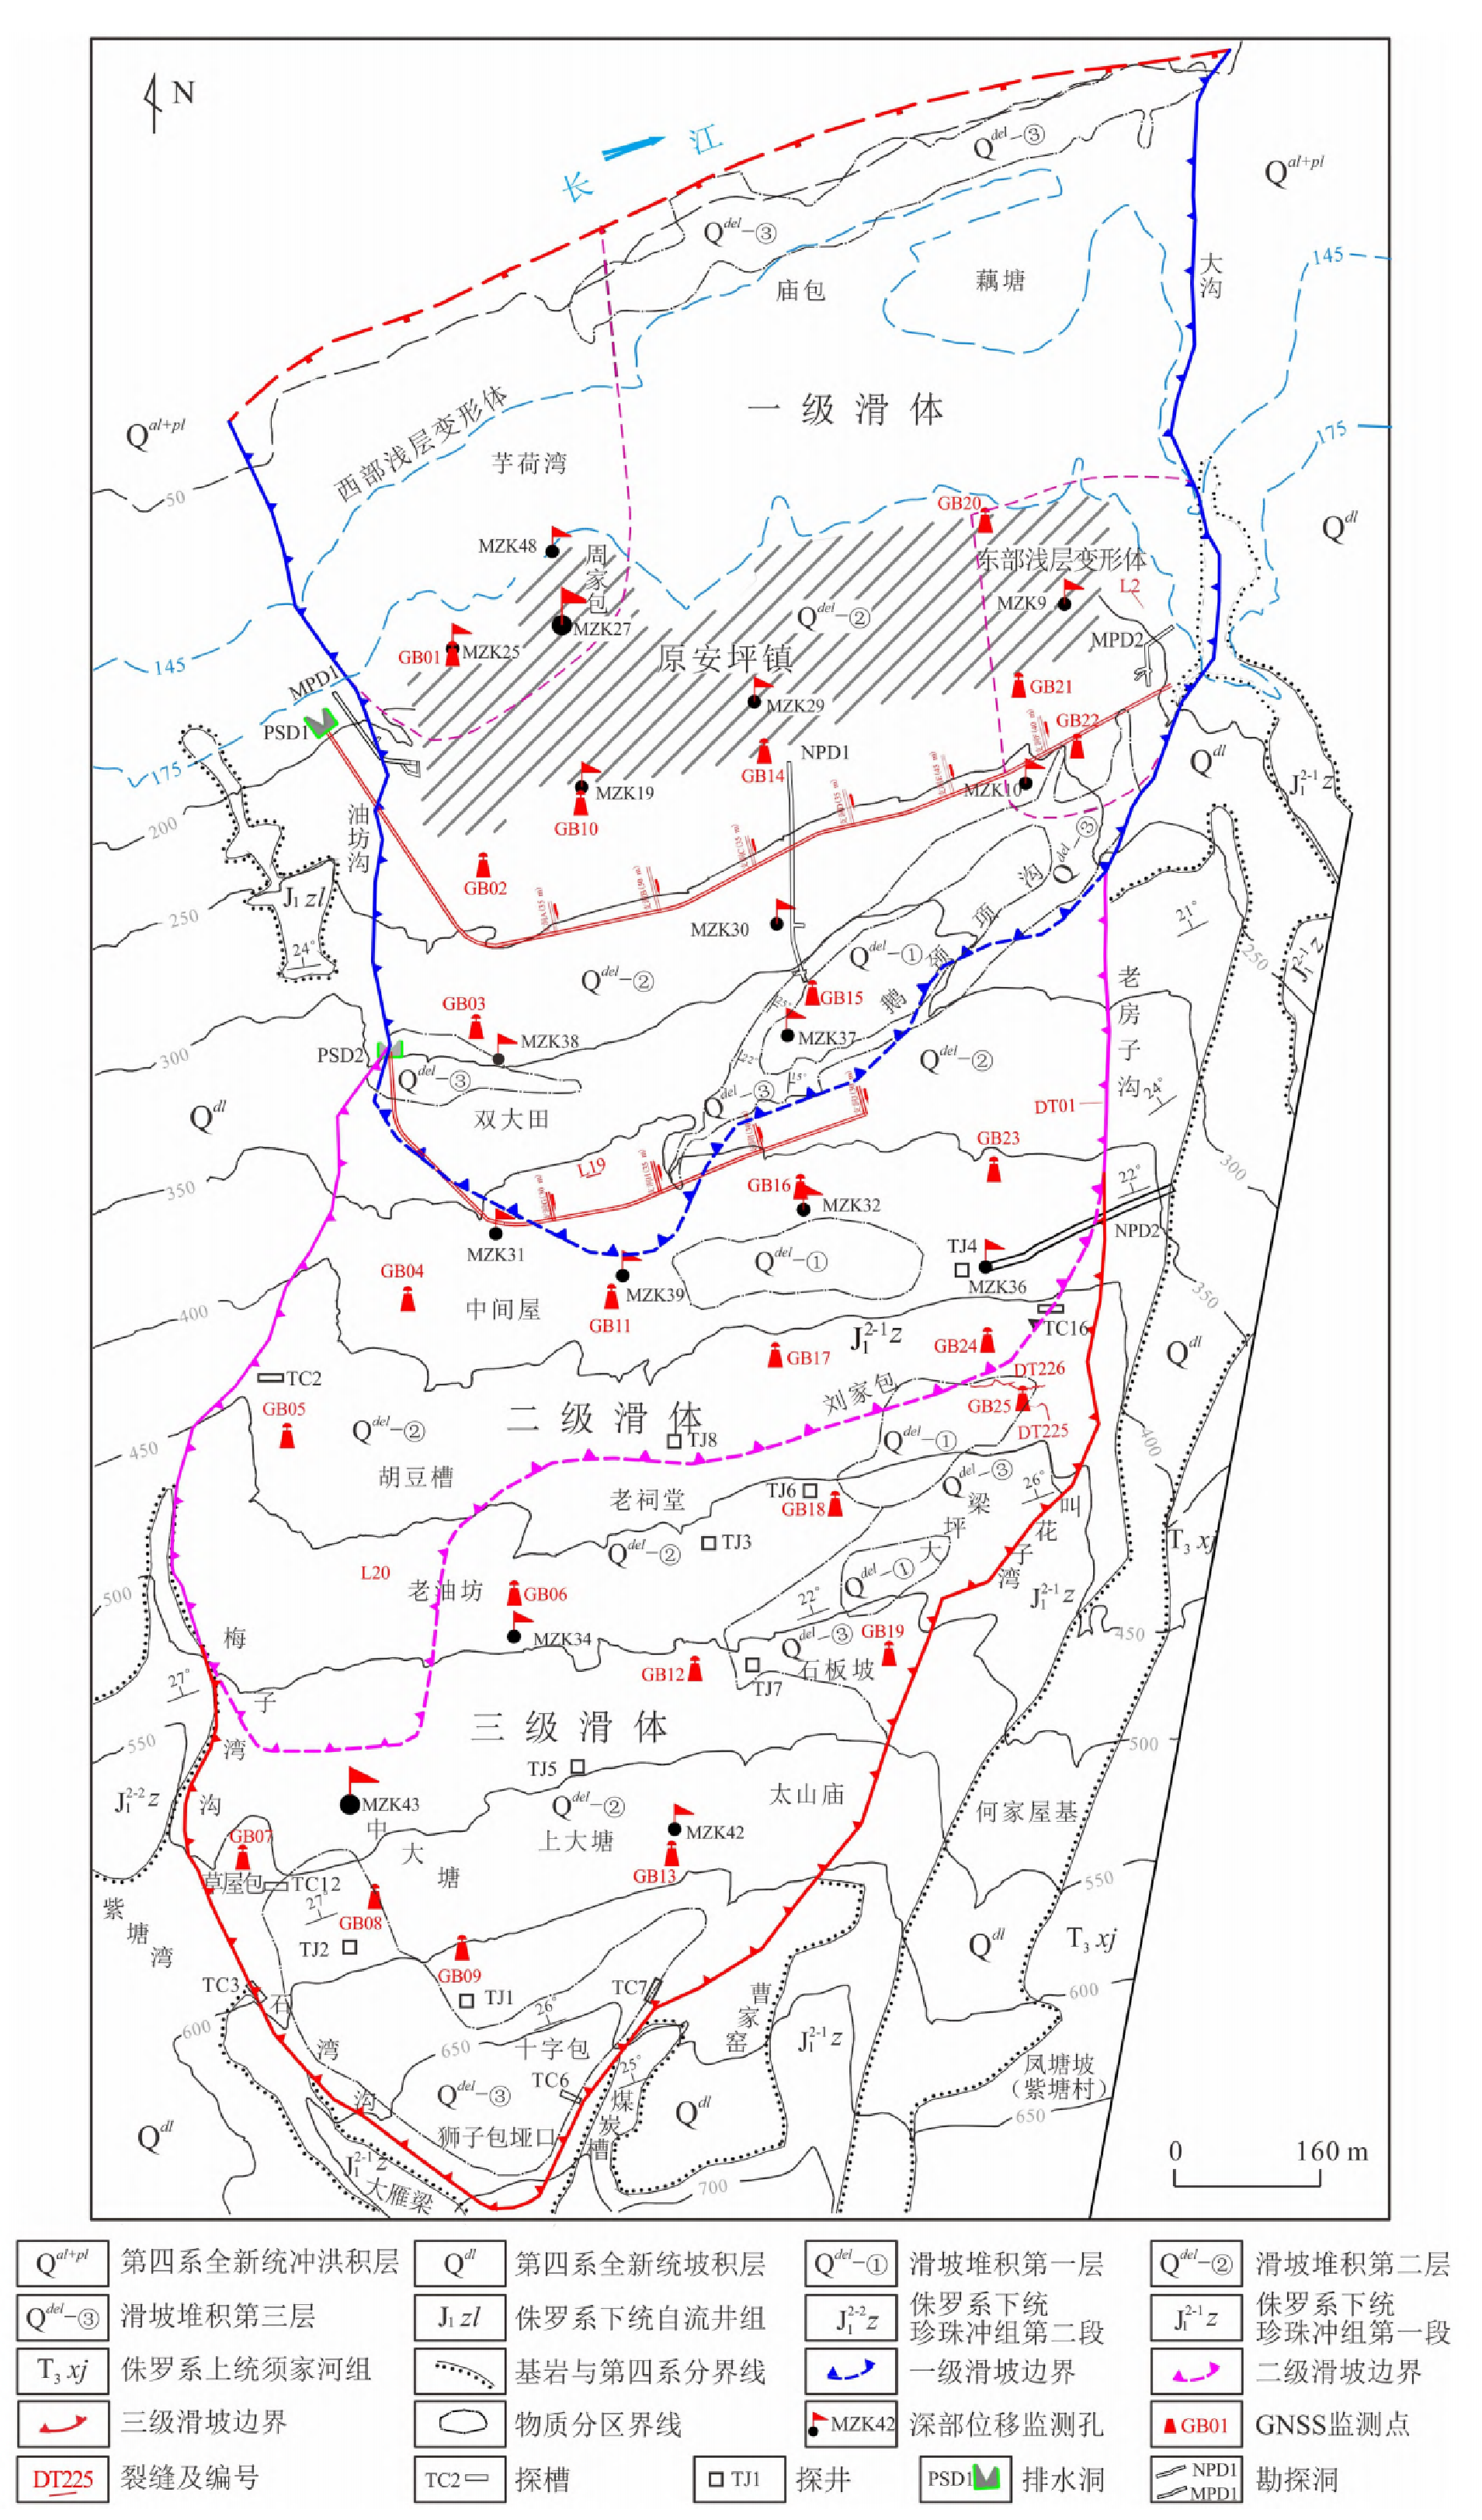
\includegraphics[width=0.9\textwidth]{figures/chapter2/Geological_map_of_Outang_landslide.pdf}
    \figcaption{藕塘滑坡地质图（赵长军等，2025）\cite{zhao2025reactivation}}{Geological Map of Outang Landslide (Zhao et al., 2025)}
    \label{fig:geology}
\end{figure}

\begin{figure}[H]
    \centering
    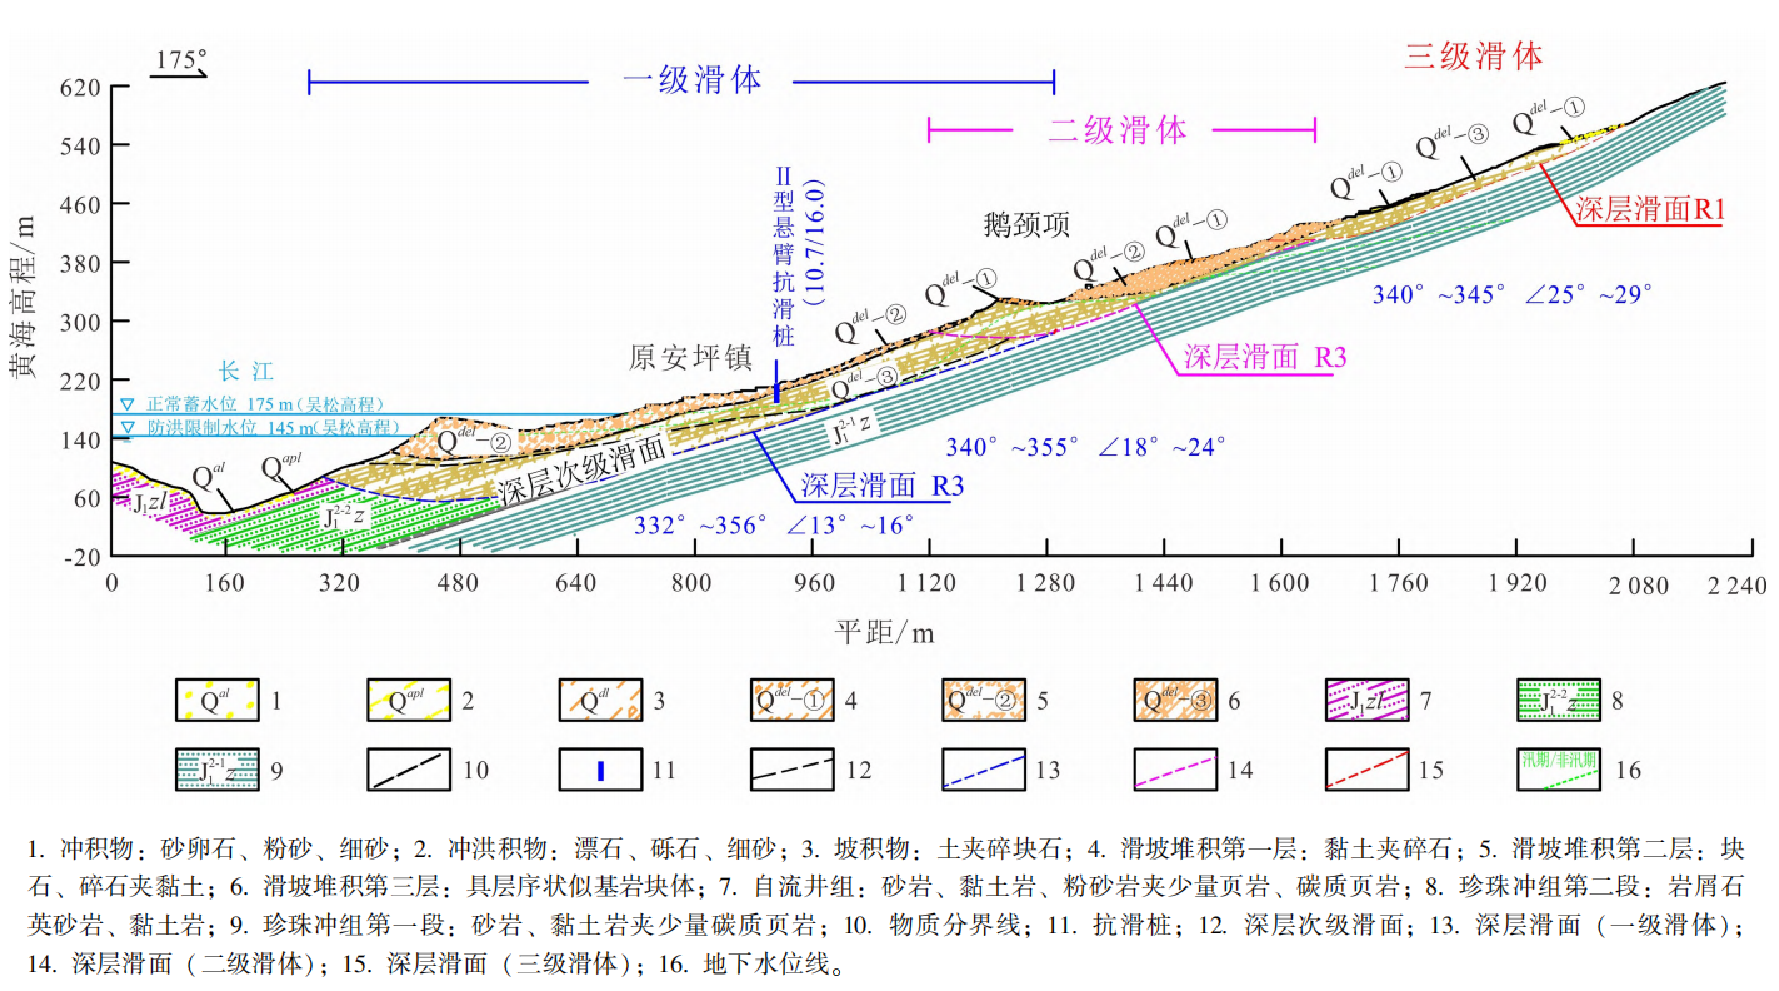
\includegraphics[width=0.9\textwidth]{figures/chapter2/Typical_geological_longitudinal_profile_of_Outang_landslide.pdf}
    \figcaption{藕塘滑坡典型地质纵剖面图（赵长军等，2025）\cite{zhao2025reactivation}}{Typical Geological Longitudinal Profile of Outang Landslide (Zhao et al., 2025)}
    \label{fig:profile}
\end{figure}

\begin{figure}[H]
    \centering
    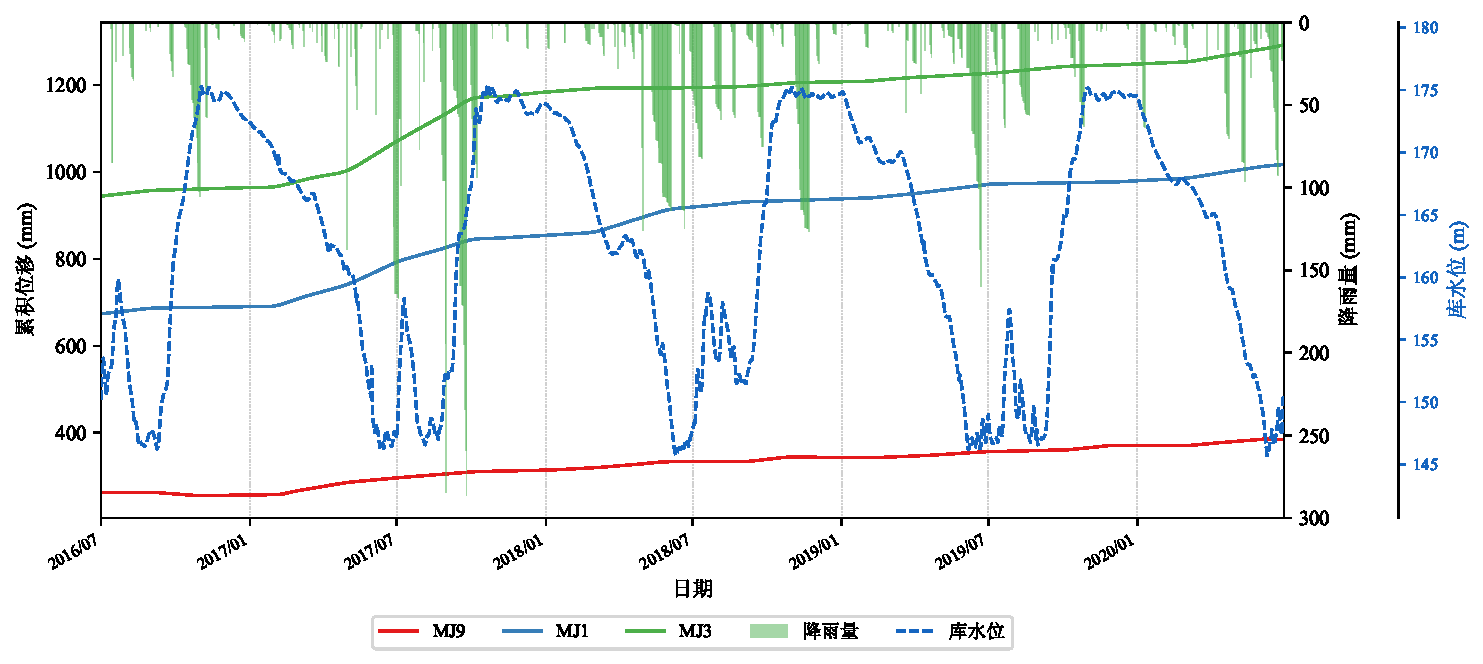
\includegraphics[width=0.95\textwidth]{figures/chapter2/monitoring_data_overview.pdf}
    \figcaption{藕塘滑坡监测数据概览（2016年7月—2020年6月）}{Overview of Monitoring Data of Outang Landslide (July 2016--June 2020)}
    \label{fig:monitoring_overview_ch2}
\end{figure}

\subsection{研究方法}

在明确了滑坡变形的潜在触发因子后，本文采用LightGBM模型探索藕塘滑坡时空位移变形与降雨、库水位、地下水位及温度等相关特征之间的关系。为了进一步提高模型的透明度和可解释性，本文结合SHAP方法对LightGBM模型进行了解释。通过对历史监测数据的分析，识别出可能导致滑坡变形的关键因素，其主要流程如下：

首先，在藕塘滑坡区域选择具有代表性的位移监测点（MJ9、MJ1、MJ3），获取长期监测数据。同时根据降雨、库水位、地下水位及气象条件选择相关的触发因子。本研究基于触发因子和监测点的位移数据训练LightGBM模型，并利用SHAP方法对模型进行解释。

在LightGBM模型训练阶段，结合滑坡体的地质背景与已知变形规律，初步筛选具有物理意义的特征因子，通过SHAP方法进一步挖掘其对模型预测的贡献与影响形式。通过SHAP贡献图、依赖图和交互图，分析不同因子对模型预测结果的贡献，包括：

    （1）贡献图分析：各触发因子对LightGBM模型位移预测的贡献大小；

    （2）依赖图分析：单个触发因子的取值变化如何影响模型的位移预测；

    （3）交互图分析：两个触发因子交互时，不同特征值组合对位移预测的影响。

通过上述“LightGBM+SHAP”方法的分析与解释，本研究从定量层面揭示了各触发因子的独立贡献、滑坡对不同触发因子变化的非线性响应和对触发因子之间的非线性耦合机制的响应，为后续滑坡时空位移预测及预警建模提供支持。

\subsubsection{算法流程}

本研究的技术路线如图~\ref{fig:algorithm_flowchart}所示，主要包括数据采集、模型训练、可解释性分析三个核心环节。

\begin{figure}[htbp]
\centering
\begin{tikzpicture}[
    scale=0.75, transform shape,
    node distance=0.8cm and 1.5cm,
    startstop/.style={rectangle, rounded corners, minimum width=2.5cm, minimum height=0.8cm, text centered, draw=black, fill=red!20, font=\footnotesize},
    process/.style={rectangle, minimum width=3cm, minimum height=0.8cm, text centered, draw=black, fill=blue!15, font=\footnotesize, align=center},
    data/.style={rectangle, rounded corners=2pt, minimum width=2.5cm, minimum height=0.7cm, text centered, draw=black, fill=yellow!20, font=\footnotesize},
    arrow/.style={thick,->,>=stealth}
]

% 第一层：开始
\node (start) [startstop] {开始};

% 第二层：数据采集
\node (data) [process, below=of start] {数据采集与预处理};

% 第三层：监测点选择
\node (select) [process, below=of data] {选择监测点（MJ9、MJ1、MJ3）};

% 第四层：特征构建
\node (feature) [process, below=of select] {构建候选特征集};

% 第五层：模型训练
\node (train) [process, below=of feature] {训练LightGBM模型};

% 第六层：SHAP分析
\node (shap) [process, below=of train] {SHAP可解释性分析};

% 分支：三种分析方法
\node (contrib) [data, below left=1cm and 1.5cm of shap] {贡献图分析};
\node (depend) [data, below=1.5cm of shap] {依赖图分析};
\node (interact) [data, below right=1cm and 1.5cm of shap] {交互图分析};

% 第七层：结果汇总
\node (result) [process, below=2cm of depend] {揭示触发因子影响机制};

% 结束
\node (end) [startstop, below=of result] {结束};

% 绘制箭头
\draw [arrow] (start) -- (data);
\draw [arrow] (data) -- (select);
\draw [arrow] (select) -- (feature);
\draw [arrow] (feature) -- (train);
\draw [arrow] (train) -- (shap);
\draw [arrow] (shap) -- (contrib);
\draw [arrow] (shap) -- (depend);
\draw [arrow] (shap) -- (interact);
\draw [arrow] (contrib) |- (result);
\draw [arrow] (depend) -- (result);
\draw [arrow] (interact) |- (result);
\draw [arrow] (result) -- (end);

\end{tikzpicture}
\figcaption{基于LightGBM+SHAP的滑坡位移预测算法流程图}{Algorithm Flowchart of Landslide Displacement Feature Analysis Based on LightGBM+SHAP}
\label{fig:algorithm_flowchart}
\end{figure}

\subsubsection{可解释机器学习模型}

\paragraph{\textbf{LightGBM模型}}

LightGBM是一种高效的梯度提升树（GBDT）框架，广泛应用于大规模机器学习任务，尤其是在数据量大且高维度特征的情况下。LightGBM通过对传统梯度提升树（GBDT）算法进行优化，提供了更高的计算效率、内存消耗更低，同时具有较强的泛化能力，适用于分类、回归、排序等多种任务。LightGBM的核心思想与传统的梯度提升方法相同，都是通过集成多个决策树来提升模型的预测性能。通过不断添加新的树来拟合误差，并结合多个树的输出，生成最终的预测结果。但LightGBM在此基础上做了一些重要的优化，使得它能够更高效地处理大规模数据集。

LightGBM在梯度提升树的基础上，采用了以下关键技术：

    （1）\textbf{直方图算法}：通过将连续特征值离散化为多个区间，在构建树时使用这些区间来选择分裂点，从而减少了计算量并提高了训练效率。特别是在处理高维数据时，直方图算法表现出显著的优势。

    （2）\textbf{叶子生长策略}：传统的GBDT采用层级生长策略，即在每一层分裂中分配节点，而LightGBM采用叶子生长策略。在这种策略中，LightGBM优先选择误差最小的叶子进行分裂，从而使得每棵树能够更好地拟合数据，尤其是在训练数据集不平衡时。

    （3）\textbf{基于梯度的单边抽样（GOSS）}：GOSS技术通过在训练过程中丢弃低梯度的样本，只保留高梯度样本来进行计算。这样可以保留最有信息的样本，提高模型训练的效率。

    （4）\textbf{互斥特征捆绑（EFB）}：EFB技术将互斥的特征捆绑在一起，从而减少了特征数量，避免了高维特征带来的计算开销。该方法对于稀疏数据集尤为有效。

LightGBM通过引入直方图算法、叶子生长策略、GOSS和EFB等优化方法，显著提高了梯度提升树在大规模数据集上的训练速度和计算效率。其对类别特征的原生支持、低内存消耗以及并行计算能力，使其在许多实际应用中成为首选的机器学习工具。通过调节超参数和特征选择，LightGBM能够在不同任务中提供优异的性能。

其LightGBM将决策树作为基学习器，表示为：
\begin{equation}
F = \{F_1, F_2, \ldots, F_n\}
\end{equation}
式中，$F_i$ 表示第$i$个学习器，$F$表示所有学习器的集合。

LightGBM通过多次的迭代不断地提升学习器的性能，每次迭代是为获得一个弱学习器，使迭代损失函数 $L(y, F_t(x))$ 最小，其公式为：
\begin{equation}
F_t(x) = F_{t-1}(x) + f_t(x)
\end{equation}
式中，$F_{t-1}(x)$、$L(y,F_{t-1}(x))$ 分别为上一次迭代获得的强学习器和损失函数。

计算损失函数的负梯度用于拟合本次迭代损失近似值，其公式为：
\begin{equation}
r_{ti} = -\left[\frac{\partial L(y_i,F_{t-1}(x_i))}{\partial F_{t-1}(x_i)}\right]
\end{equation}

目标函数通常为平方差，使用平方差近似拟合为：
\begin{equation}
f_t(x) = \arg\min \sum_i(r_{ti} - f(x_i))^2
\end{equation}

最终获得本次迭代获得的强学习器为：
\begin{equation}
F_t(x) = F_{t-1}(x) + \eta f_t(x)
\end{equation}

LightGBM模型通过以上方式不断更新，采用histogram算法减少内存的使用和计算的复杂度，使用Leaf-wise的叶子优先生长策略，并通过设置最大树深限制其结构复杂度。该方法能够在保证精度的前提下加快收敛速度，相较于传统的Level-wise方法更适用于大规模数据场景。基于梯度的单边采样（GOSS）和互斥特征捆绑（EFB）减少训练时间。

\paragraph{\textbf{SHAP解释模型}}

SHAP是基于博弈论的解释方法，用于解释机器学习模型的预测结果，量化了每个特征对单一预测结果的贡献。SHAP值为每个特征分配一个值，表示该特征对某一预测结果的贡献度。它是一种非常强大的工具，能够帮助我们理解模型是如何根据输入特征做出预测的，尤其对于复杂的模型（如LightGBM、XGBoost等树模型）尤为有效。对于给定的输入样本$x$有着$N$个解释变量，解释模型$g$表示特征贡献的线性函数：
\begin{equation}
g(x') = \varphi_0 + \sum_{j=1}^{N} \varphi_j x'_j
\end{equation}
式中$\varphi_0$代表模型输出的基本值，$N$是所有输入特征的总数，$x'_j$是二元变量，表示第$j$个预测变量是否存在（$x'_j=1$）或不存在（$x'_j=0$）。$\varphi_j \in \mathbb{R}$是样本$x$中第$j$个的SHAP值（即特征属性）。
\begin{equation}
\varphi_j = \sum_{S \subseteq N \setminus \{j\}} \frac{|S|!(N-|S|-1)!}{N!}[f(S\cup\{j\})-f(S)]
\end{equation}
其中，$S$表示输入的解释变量的子集，$f(S\cup\{j\})$和$f(S)$分别是包含和不包含第$j$个特征时模型的预测值。

\begin{equation}
\varphi_{j,k} = \sum_{S \subseteq N \setminus \{j,k\}} \frac{|S|!(N-|S|-2)!}{2(N-1)!} \nabla_{jk}(S)
\end{equation}
此外，为了量化变量之间的配对相互影响，SHAP交互值被引入用于度量特征之间的交互影响。
\begin{equation}
\nabla_{jk}(S) = f_x(S\cup x_j, x_k) - f_x(S\cup x_j) - f_x(S\cup x_k) + f_x(S)
\end{equation}
当$j \neq k$时，由于特征$j$和$k$之间的SHAP交互值平均分配到$\varphi_{j,k}$和$\varphi_{k,j}$中，因此总的交互影响是$\varphi_{j,k}$和$\varphi_{k,j}$的和。每个变量的主要影响是通过从SHAP值中减去SHAP交互值来确定的。

\subsubsection{候选特征选择}

滑坡的候选因素应结合物理机理与数据驱动分析两方面进行综合选取。从物理机制角度来看，滑坡的发生和发展过程通常受多种自然环境与工程活动因素的共同作用，这些因素会影响坡体的应力状态、地下水变化和土体结构稳定性。特别是库水位变化和强降雨事件，常常是诱发滑坡活动的直接触发因素。坡度、地层岩性、软弱结构面等内在地质条件，则决定了滑坡的易发性与演化路径。

在本次的初始特征选择中，参考了前人的研究成果，针对藕塘滑坡的时空位移预测任务，初步筛选出基于时间窗口的滞后特征，包括历史位移、降雨、库水位、地下水位及气象因子，如表\ref{tab:candidate_features}所示。

\begin{table}[htbp]
\centering
\tabcaption{触发特征的候选因子}{Candidate Triggering Features for Landslide Displacement}
\label{tab:candidate_features}
\begin{tabular}{ll}
\toprule
候选因素类别 & 描述 \\
\midrule
历史位移特征 & 过去5天的位移值disp$(t-5)$至disp$(t-1)$ \\
降雨特征 & 过去5天的日降雨量Rainfall$(t-5)$至Rainfall$(t-1)$ [mm] \\
库水位特征 & 过去5天的库水位RWL$(t-5)$至RWL$(t-1)$ [m] \\
地下水位特征 & 过去5天的地下水位GWT$(t-5)$至GWT$(t-1)$ [m] \\
平均温度特征 & 过去5天的平均温度aveT$(t-5)$至aveT$(t-1)$ [°C] \\
最低温度特征 & 过去5天的最低温度minT$(t-5)$至minT$(t-1)$ [°C] \\
最高温度特征 & 过去5天的最高温度maxT$(t-5)$至maxT$(t-1)$ [°C] \\
露点特征 & 过去5天的露点DP$(t-5)$至DP$(t-1)$ [°C] \\
相对湿度特征 & 过去5天的相对湿度RH$(t-5)$至RH$(t-1)$ [\%] \\
监测点标识 & 监测点one-hot编码（MJ9、MJ1、MJ3） \\
\bottomrule
\end{tabular}
\end{table}

\subsubsection{藕塘滑坡变形机制分析}

藕塘滑坡作为三峡库区典型的水库型滑坡，其位移过程表现出明显的阶跃特征，即在特定时间段内位移突增，而在其他时间段相对稳定。这类位移特征在库区滑坡中具有代表性，通常受到周期性库水位变化和突发性降雨过程的共同驱动。藕塘滑坡地质背景复杂，主要分布于软弱堆积层或顺层结构发育的坡体中，地层结构和物理力学性质使其对外部水动力扰动极为敏感。此外，其所处区域的库水位调控方式及年降雨量水平也具有典型性。因此，在地质构造、水文气象条件相近的背景下，藕塘滑坡呈现出独特的变形响应特征。为深入理解三峡库区滑坡位移的形成与演化规律，有必要进一步分析其滑坡变形机制，揭示库水位与降雨在不同阶段如何共同作用于滑坡体，驱动滑坡变形及失稳过程。

从三峡库区典型滑坡的变形演化过程来看，滑坡体的阶跃式位移通常源于降雨和库水位变化的耦合作用机制。这一机制主要通过以下几种路径对滑坡变形产生影响：

    （1）\textbf{库水位变化引起的软化与卸载作用}：在水库蓄水或调控过程中，库水位的周期性涨落会引发滑坡体前缘的软化和卸载效应。当库水位快速下降时，坡脚支撑力减弱，滑坡体前缘土体失去约束，同时滑坡体内部由于仍处于高孔隙水压力状态，造成剪切应力增大，滑坡体发生应力重分布，进而引发滑动。特别是对于具有顺层结构或软弱夹层的滑坡体，该过程更加显著。

    （2）\textbf{降雨入渗引起的孔隙水压力升高}：持续或强降雨会导致雨水大量入渗，改变滑坡体内部的水文条件。随着入渗深度的增加，孔隙水压力迅速上升，有效应力降低，滑动面抗剪强度减弱，从而诱发滑坡位移。此外，强降雨还可能造成坡面径流侵蚀或沟蚀作用，削弱滑坡体的表层稳定性，加速变形。

    （3）\textbf{库水位与降雨的协同效应}：研究发现，单一因素（仅降雨或仅水位变化）难以充分解释大部分滑坡的突跳式位移行为，而库水位下降与强降雨同时发生时，往往引发滑坡的突发性变形。这是由于两种作用机制相互叠加，共同降低滑坡体的稳定性。例如，在库水位下降期遇上强降雨事件，不仅坡体抗剪强度削弱，而且坡脚卸载增强，极易导致大位移的发生。罗世林等\cite{luo2024response}通过监测数据分析、相关性理论及离散元数值模拟，系统揭示了库水—降雨耦合作用下堆积层滑坡的响应机理，证实了库水位变动与降雨入渗的协同效应是触发此类滑坡阶跃变形的关键机制。

    （4）\textbf{地质结构条件的调控作用}：上述变形机制的实际表现形式，还受到滑坡体地质构造的影响。藕塘滑坡广泛发育软弱层或顺倾结构带，岩土体抗剪强度低，对水敏感性强，更容易在外部水动力作用下发生变形破坏。同时，滑带土中黏粒含量高、渗透性差，也促进孔压积聚，加剧滑坡体失稳。

综合前人研究成果可知，藕塘滑坡的变形机理主要体现在以下几个方面：

    （1）库水位变化是滑坡变形的核心驱动因素，其中尤以水位快速下降引发的动水压力变化对滑坡体稳定性的影响最为显著；

    （2）降雨通过增加孔隙水压力、软化岩土体等作用机制，与库水位变化产生叠加效应，进一步加剧滑坡变形过程；

    （3）滑坡体渗透性的差异性也决定了其对水位变化的响应程度，渗透性较差的滑坡在水位骤降时更易出现失稳滑动现象。

\subsection{结果及讨论}

\subsubsection{数据准备与模型构建}

本研究基于藕塘滑坡区域的长期监测数据，选取了三个具有代表性的位移监测点（MJ9、MJ1、MJ3）进行分析。监测数据时间跨度覆盖了多个完整的库水位调度周期，包含了丰富的滑坡变形信息。数据集包括日尺度的位移监测值、降雨量、库水位、地下水位以及气象要素（平均温度、最低温度、最高温度、露点、相对湿度）等多维度信息。

在样本构造阶段，采用时间窗口为5天的滑动窗口方法，将历史时序数据转化为监督学习样本。对于每个监测点，输入特征包括：该点过去5天的位移值、过去5天的环境因子（降雨、库水位、地下水位、温度、湿度等）以及监测点的one-hot编码。回归任务的目标变量为当天的位移增量（$\Delta u = u_t - u_{t-1}$），用于预测滑坡的时空位移变化；分类任务的目标变量基于位移增量是否超过固定阈值0.3 mm来定义，用于判定是否进入预警状态。为了严格防止模型评估中出现隐性的数据泄漏，本研究仅基于训练集的统计分布特征来划定预警阈值。通过对训练集数据的统计分析，设定0.3 mm为分类任务的固定阈值。该数值接近MJ9监测点训练集的95\%分位数，同时处于MJ1和MJ3监测点训练集的75\%至90\%分位数之间。这一基于先验训练数据的固定阈值设定，不仅有效捕捉了异常变形信号，还避免了在时序交叉验证中使用全局统计量带来的未来数据泄漏风险，确保了模型评估的严谨性与客观性。

在模型验证策略上,本研究采用5折时序交叉验证（TimeSeriesSplit）对模型性能进行评估。时序交叉验证严格保持数据的时间顺序，每一折中训练集始终位于测试集之前，从而避免了随机划分可能导致的“未来数据泄漏”问题，真实模拟了实际预测场景中的时序依赖关系。针对预警样本在时间维度上分布不均匀的问题（预警事件往往集中在特定时期），本研究在每一折的训练阶段引入SMOTE（Synthetic Minority Over-sampling Technique）过采样技术，仅对训练集中的少数类样本进行合成扩充，以缓解类别不平衡对分类模型学习的影响。需要强调的是，SMOTE操作严格限定在训练集内部，测试集保持原始分布不变，确保评估结果的客观性。由于LightGBM是基于树的模型，对特征尺度不敏感，因此无需进行标准化处理。

\subsubsection{模型性能评估}

\paragraph{（1）时空位移预测模型（回归任务）}

\begin{sloppypar}
基于LightGBM构建的回归模型用于预测藕塘滑坡的时空位移增量。模型采用了较为保守的超参数设置，包括较小的树深度（max\_depth=3）和叶子节点数（num\_leaves=4），以及适度的正则化参数（lambda\_l1=0.2, lambda\_l2=0.2），以防止过拟合并提高模型的泛化能力。同时设置特征采样比例（feature\_fraction=0.8）和样本采样比例（bagging\_fraction=0.8），进一步增强模型的鲁棒性。
\end{sloppypar}

经5折时序交叉验证，回归模型在训练集和测试集上的均方误差（MSE）分别为$0.0466 \pm 0.0492$和$0.0780 \pm 0.0641$。测试集上的MSE表明模型具有一定的预测精度，能够捕捉滑坡位移增量的变化趋势。训练集与测试集误差的差异反映了时序预测任务的固有难度——由于预警事件在时间维度上分布不均匀，不同时期的位移增量变化幅度存在较大差异，导致各折之间的标准差较大。总体而言，模型在严格的时序验证框架下展现出合理的泛化性能。

\paragraph{（2）预警判定模型（分类任务）}

基于LightGBM构建的分类模型用于判定滑坡是否进入预警状态。模型采用了二分类目标函数，并综合运用两种类别平衡策略：一是在训练集上使用SMOTE过采样技术合成少数类样本，二是设置scale\_pos\_weight=5对正样本赋予更高的损失权重。分类模型采用了num\_leaves=8、max\_depth=3的树结构，以及较强的正则化参数（lambda\_l1=0.3, lambda\_l2=0.3），在模型复杂度与泛化能力之间取得平衡。

经5折时序交叉验证（其中2折因测试集无正样本而跳过），分类模型在有效折上的测试集AUC为$0.6795 \pm 0.1181$，召回率（Recall）为$0.7623 \pm 0.3362$，精确率（Precision）为$0.2970 \pm 0.2476$，F1分数为$0.3935 \pm 0.2790$。训练集AUC为$0.9423 \pm 0.0405$，表明模型具有较强的学习能力。

从预警系统的实际应用角度分析，模型的召回率达到76.23\%，意味着超过四分之三的真实预警事件能够被模型成功识别，这对于灾害预警系统而言具有重要的实用价值——在滑坡预警场景中，漏报的代价远高于误报。测试集AUC的波动（标准差0.1181）主要源于预警事件在时间维度上的非均匀分布特征，这是时序预测任务的固有挑战。需要指出的是，部分折次因测试时段恰好处于滑坡稳定期而无预警样本，这一现象本身也反映了滑坡变形的阶跃性特征。相比于采用随机打乱的分层交叉验证可能获得的虚高指标，本研究坚持使用严格的时序验证策略，所得结果更能真实反映模型在实际预测场景中的表现。

\subsubsection{SHAP可解释性分析}

为了深入理解模型的预测机制，揭示各输入特征对滑坡位移预测的贡献，本研究采用SHAP方法对训练好的LightGBM模型进行了可解释性分析。具体而言，选取时序交叉验证中最后一折训练得到的模型作为解释对象，该折模型使用了最大规模的训练数据，能够最充分地学习特征与位移之间的映射关系。

\paragraph{\textbf{回归模型的SHAP分析}}

图\ref{fig:shap_regression}展示了回归模型的SHAP特征重要性总结图。从图中可以看出，对滑坡位移增量预测贡献最大的特征主要包括：

    （1）\textbf{历史位移特征}：过去5天的位移值（特别是disp$(t-1)$和disp$(t-2)$）对当前位移增量的预测具有显著贡献。这符合滑坡变形的时序连续性特征，即近期的位移状态对未来位移具有强烈的指示作用。

    （2）\textbf{库水位特征}：库水位的滞后特征（RWL$(t-1)$至RWL$(t-5)$）在模型预测中占据重要地位。SHAP值的分布显示，库水位的变化对滑坡位移具有复杂的非线性影响。当库水位较低或快速下降时，SHAP值倾向于正值，表明这些条件会促进位移增量的增大；而当库水位较高且稳定时，SHAP值倾向于负值，表明滑坡处于相对稳定状态。

    （3）\textbf{降雨特征}：降雨量的滞后特征（Rainfall$(t-1)$至Rainfall$(t-5)$）也显示出明显的贡献。较大的降雨量对应较高的正向SHAP值，表明强降雨会显著增加滑坡位移增量。这与降雨入渗导致孔隙水压力升高、有效应力降低的物理机制相吻合。

    （4）\textbf{地下水位特征}：地下水位（GWT）的变化对滑坡位移也有重要影响。地下水位的升高通常对应正向SHAP值，表明地下水位上升会增加滑坡变形的风险。

    （5）\textbf{气象特征}：温度、露点、相对湿度等气象特征虽然贡献相对较小，但仍在模型中发挥作用。这些特征可能通过影响土体的冻融循环、蒸发蒸腾等过程，间接影响滑坡的稳定性。

    （6）\textbf{监测点标识}：不同监测点的one-hot编码特征也显示出一定的贡献，表明不同位置的监测点对外部触发因素的响应存在差异，这与滑坡体内部的地质结构异质性有关。

\begin{figure}[htbp]
\centering
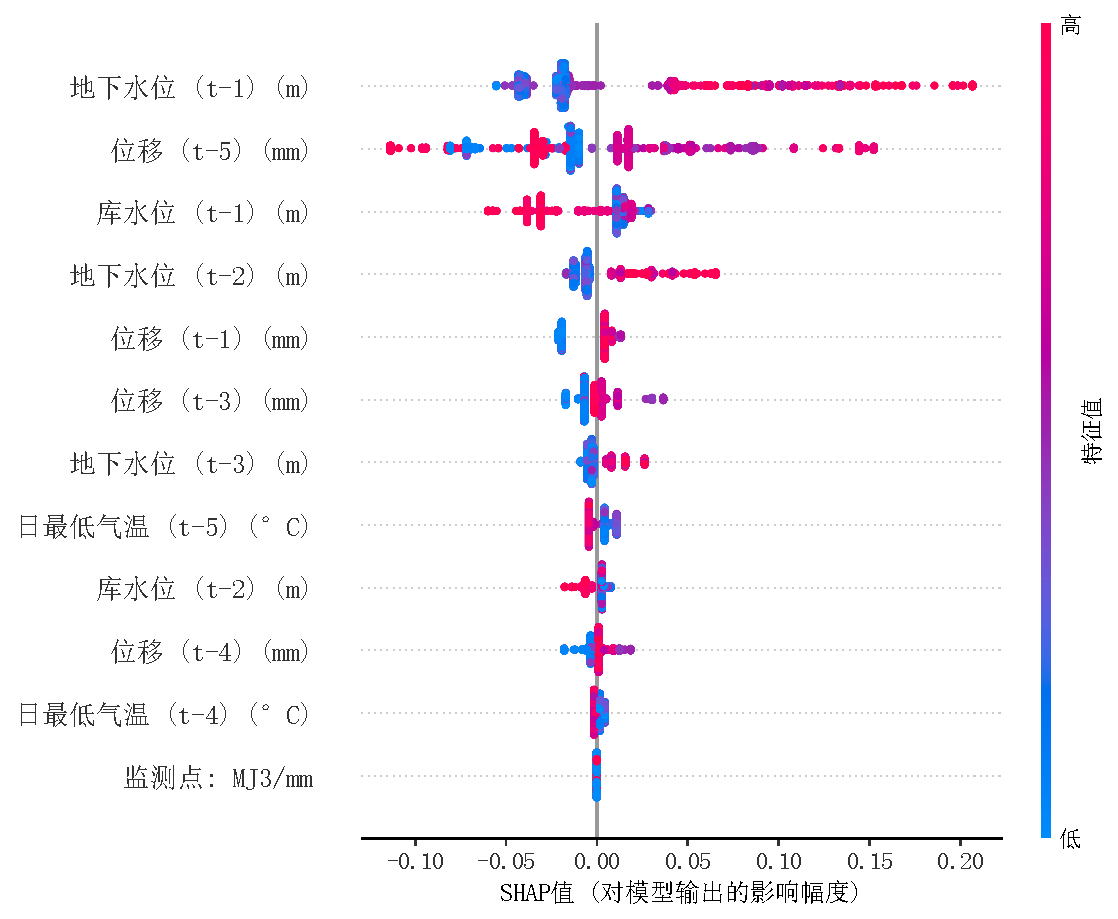
\includegraphics[width=0.8\textwidth]{figures/chapter2/shap_summary_regression.pdf}
\figcaption{SHAP特征重要性总结图（回归模型）}{SHAP Feature Importance Summary Plot (Regression Model)}
\label{fig:shap_regression}
\end{figure}

\paragraph{\textbf{分类模型的SHAP分析}}

图\ref{fig:shap_classification}展示了分类模型的SHAP特征重要性总结图（针对预警状态）。从图中可以看出，促使滑坡进入预警状态的关键因子包括：

    （1）\textbf{历史位移特征}：与回归模型类似，近期的位移值（特别是disp$(t-1)$）对预警判定具有最强的指示作用。较大的历史位移值对应较高的正向SHAP值，表明滑坡已经处于活跃变形状态，进入预警的概率显著增加。

    （2）\textbf{库水位特征}：库水位的快速下降是触发预警的重要因素。SHAP分析显示，当库水位处于较低水平或短期内大幅下降时，模型倾向于判定为预警状态。这与库水位下降引起的坡脚卸载和动水压力变化机制相一致。

    （3）\textbf{降雨特征}：强降雨事件是触发预警的另一关键因素。当短期内累积降雨量较大时（特别是Rainfall$(t-1)$和Rainfall$(t-2)$），SHAP值显著增大，表明模型识别到了降雨诱发滑坡变形的风险。

    （4）\textbf{地下水位特征}：地下水位的快速上升也是预警的重要指标。这反映了降雨入渗和库水位变化对地下水动态的综合影响。

    （5）\textbf{特征交互效应}：分类模型的SHAP分析还揭示了特征之间的交互效应。例如，当库水位下降与强降雨同时发生时，两者的协同作用会显著增加进入预警状态的概率，这与前述的耦合作用机制相吻合。

\begin{figure}[htbp]
\centering
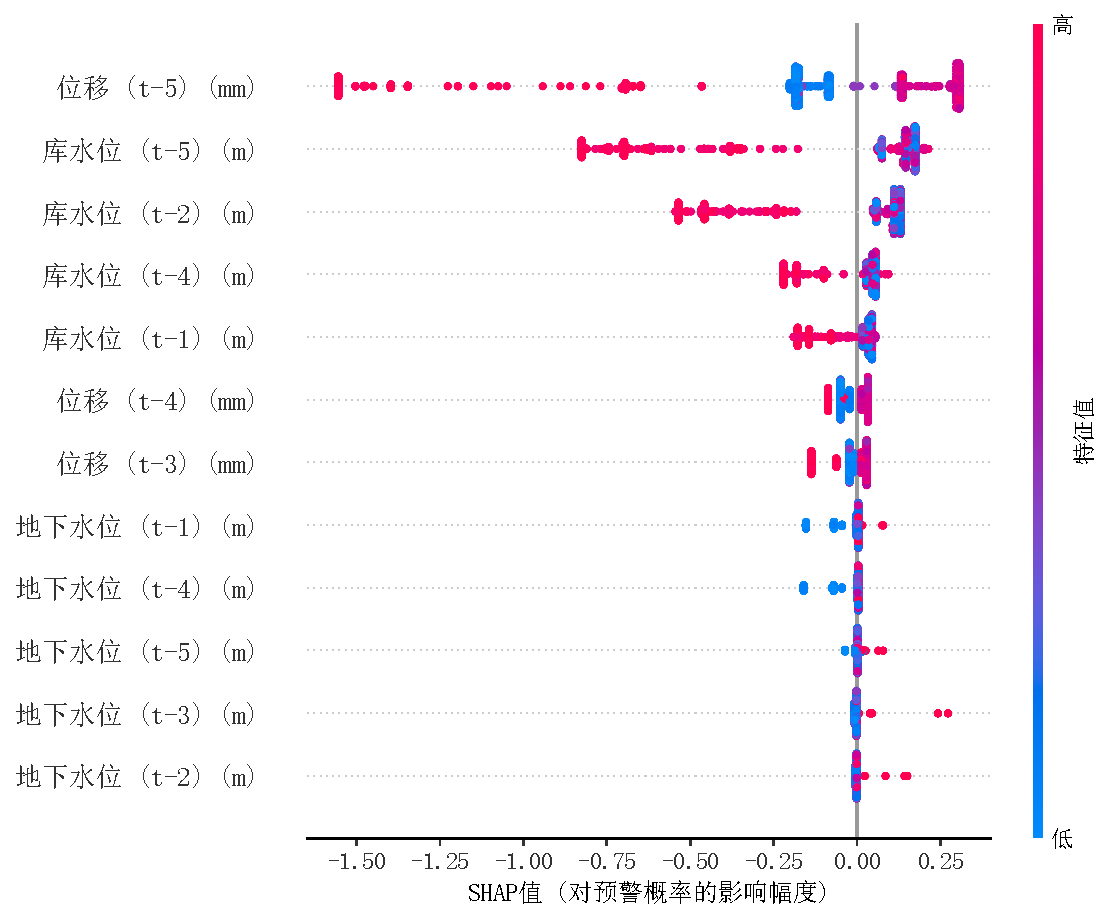
\includegraphics[width=0.8\textwidth]{figures/chapter2/shap_summary_classification.pdf}
\figcaption{SHAP特征重要性总结图（分类模型）}{SHAP Feature Importance Summary Plot (Classification Model)}
\label{fig:shap_classification}
\end{figure}

\subsubsection{讨论}

\paragraph{\textbf{（1）特征重要性与物理机制的一致性}}

SHAP分析结果与藕塘滑坡的物理变形机制高度一致。库水位变化和历史位移累积效应作为最重要的触发因子，在SHAP贡献图中占据主导地位，这验证了滑坡变形的累积驱动机制假设。气温变化的较高贡献则反映了环境温度对滑坡稳定性的间接影响。地下水位作为连接外部触发因素（降雨、库水位）与滑坡内部响应的桥梁，其重要性也得到了SHAP分析的支持。

\paragraph{\textbf{（2）非线性响应特征}}

SHAP依赖图揭示了滑坡对触发因素的非线性响应。例如，库水位对滑坡位移的影响并非简单的线性关系，而是存在阈值效应：当库水位低于某一临界值或下降速率超过某一阈值时，滑坡变形会显著加剧。类似地，降雨量也存在触发阈值，只有当累积降雨量超过一定值时，才会对滑坡位移产生显著影响。

\paragraph{\textbf{（3）时空差异性}}

不同监测点的one-hot编码特征在SHAP分析中显示出一定的贡献，表明滑坡体内部存在时空差异性。这种差异性可能源于：(1)不同位置的地质结构差异（如滑带厚度、岩土体性质）；(2)不同位置对外部触发因素的响应敏感性差异；(3)不同位置的排水条件和渗流路径差异。这一发现强调了在滑坡预测和预警中考虑空间异质性的重要性。

\paragraph{\textbf{（4）预警模型的实用价值}}

分类模型的SHAP分析为滑坡预警系统的构建提供了明确的指导。通过识别促使进入预警状态的关键因子及其阈值，可以建立基于多因子联合判定的预警准则。例如，当历史位移增量较大、库水位快速下降且遭遇强降雨时，应立即发布预警信号。模型在严格时序验证下的召回率达到76.23\%，表明超过四分之三的真实预警事件能够被成功捕捉，这对于“宁可误报、不可漏报”的灾害预警原则具有重要意义。这种基于可解释机器学习的预警方法，相比传统的经验阈值法，具有更强的科学性和可靠性。

\paragraph{\textbf{（5）模型的局限性与改进方向}}

尽管本研究构建的LightGBM模型在藕塘滑坡的时空位移预测和预警判定中展现出一定的预测能力，但仍存在以下局限性：(1)时序交叉验证中，由于预警事件在时间维度上的非均匀分布，部分折次的测试集缺乏正样本，导致有效评估折数减少，模型性能指标的波动较大；(2)模型基于历史数据训练，对于超出训练集范围的极端事件（如特大暴雨、异常库水位调度）的预测能力有待验证；(3)模型未考虑滑坡体的物理力学参数（如抗剪强度、渗透系数）的时变性；(4)模型的时间窗口（5天）是基于经验选择的，可能不是最优值。未来研究可以考虑：(1)引入物理模型与数据驱动模型的耦合，提高模型的物理可解释性和外推能力；(2)采用自适应时间窗口或多尺度时间窗口，以更好地捕捉不同时间尺度的变形特征；(3)结合深度学习方法（如LSTM、Transformer）进一步提升模型对长期依赖关系的建模能力；(4)探索更精细的时序划分策略，如滑动窗口验证或基于变形阶段的分段验证，以提高模型评估的稳定性。

\subsection{本章小结}

本章基于LightGBM模型，探讨了藕塘滑坡的时空位移与降雨、库水位、地下水位及气象因子等关键影响因子之间的关系，并采用SHAP方法对模型进行可解释性分析。研究从SHAP特征贡献、单个影响因子对模型预测的影响及影响因子之间的交互关系三个方面展开，系统揭示了影响因子的重要性排序、单一特征的影响模式以及影响因子间的协同效应，为滑坡时空位移的精准预测和预警提供了科学依据。主要结论如下：

    （1）构建了基于LightGBM的藕塘滑坡时空位移预测模型和预警判定模型，并采用严格的5折时序交叉验证结合SMOTE过采样技术进行模型评估。回归模型在测试集上的MSE为$0.0780 \pm 0.0641$，能够有效预测滑坡的位移增量；分类模型在测试集上的AUC为$0.6795 \pm 0.1181$，召回率达到76.23\%，能够识别大部分真实预警事件。时序验证策略严格避免了数据泄漏，所得结果真实反映了模型在实际预测场景中的性能，为滑坡监测预警系统的构建提供了可靠的技术支撑。

    （2）SHAP贡献图识别了影响滑坡位移预测的核心特征，直观展示了不同触发因子的特征值对模型预测的影响。对于藕塘滑坡，影响位移预测最大的特征包括：历史位移值（disp$(t-1)$至disp$(t-5)$）、库水位（RWL$(t-1)$至RWL$(t-5)$）、降雨量（Rainfall$(t-1)$至Rainfall$(t-5)$）以及地下水位（GWT$(t-1)$至GWT$(t-5)$）。这些主控因子与阶跃型滑坡的变形机理基本吻合，验证了滑坡变形的累积驱动机制假设。

    （3）SHAP依赖图进一步揭示了单个影响因子对预测结果的具体影响模式，展现了特征值变化对滑坡位移的非线性作用及潜在的阈值效应。研究发现，库水位较低或快速下降、降雨量超过特定阈值、地下水位快速上升等条件会显著加剧滑坡位移的发生。这些发现为建立基于多因子联合判定的预警准则提供了定量依据。

    （4）SHAP交互图揭示了不同特征之间的相互作用，分析了特定特征在不同条件下对滑坡位移的增强或削弱效应，为深入理解滑坡演化机理提供了新视角。对于藕塘滑坡，降雨与库水位的联合作用中，当库水位下降与强降雨同时发生时，两者的协同效应会显著增加滑坡进入预警状态的概率。

    （5）本章采用的“LightGBM+SHAP”方法有效克服了传统机器学习模型“黑盒”特性的不足，提升了特征选择的科学性与模型的可解释性。在模型验证方面，采用严格的时序交叉验证策略并结合SMOTE过采样技术处理类别不平衡问题，确保了评估结果的学术严谨性和实际可信度。通过“先验知识指导初筛+数据算法量化验证”的研究策略，不仅实现了对候选因子的精准筛选与排序，更为后续滑坡时空位移预测及预警模型的优化提供了数据支持和理论依据。

本章的研究成果为三峡库区及类似地质环境下的滑坡监测预警提供了可借鉴的技术路线和方法体系，具有重要的科学意义和工程应用价值。

\section{基于位移运动学特征的滑坡位移预测模型研究}

\subsection{前言}

在第二章中，本研究通过LightGBM模型结合SHAP方法，系统地识别并量化了影响藕塘滑坡位移变形的关键触发因子，包括降雨、库水位、地下水位及气象因素等。这些分析揭示了滑坡位移与外部触发因子之间的复杂非线性关系，为理解滑坡变形机制提供了重要依据。然而，第二章的工作主要聚焦于特征重要性分析，尚未构建位移预测模型。

水库滑坡的位移演化过程具有复杂的非线性时变特性和显著的空间协同变形特征。滑坡体不同部位的位移并非孤立演化，而是存在明显的空间关联性：后缘推力区的变形会传递至中部主滑区，进而影响前缘阻滑区的响应。这种空间协同变形特征为位移预测提供了重要的信息来源。基于多个监测点的历史位移序列进行联合预测，能够充分利用滑坡体的空间运动学特征，相比单点自回归模型具有更强的预测能力。

为此，本章引入长短期记忆网络（LSTM）作为核心预测模型。LSTM通过其独特的门控机制，能够有效捕捉滑坡位移时间序列中的长期依赖关系。相比传统的时间序列方法，LSTM能够突破传统马尔可夫假设的限制，自适应地赋予不同时间步历史信息相应的权重，特别适合处理滑坡位移这类具有复杂非线性特征的时序预测问题。

此外，传统的确定性点预测难以量化预测的可靠性，在工程应用中存在局限性。为了提供更全面的预测信息，本章提出基于多次运行的概率预测框架。通过对LSTM模型进行50次独立训练，每次使用不同的随机种子初始化参数，收集50次预测结果形成统计分布。该方法不仅能够输出位移的期望值，还能同时给出不同置信水平下的预测区间，客观量化模型的认知不确定性，为滑坡灾害的风险评估与预警决策提供更加全面的信息支持。

本章以藕塘滑坡MJ9、MJ1、MJ3三个代表性监测点为研究对象，利用滑坡体上多个关键监测点的历史位移序列作为空间运动学输入特征，验证所提方法的有效性与可靠性，为后续章节的预警研究奠定基础。


\subsection{方法原理}

本章提出的LSTM概率预测模型主要包括两个核心模块：LSTM时序预测模块和概率预测模块。模型基于滑坡体多个监测点的历史位移序列，利用空间协同变形特征进行联合预测。具体而言，选取MJ9、MJ1、MJ3、ATU4四个关键监测点的历史位移时间序列作为输入，构建LSTM时序预测模型，分别预测MJ9、MJ1、MJ3三个监测点未来时刻的趋势项位移；通过50次独立运行获得预测的统计分布，输出不同置信水平下的预测区间，实现位移的概率预测。

\subsubsection{算法流程}

本研究的技术路线如图~\ref{fig:lstm_algorithm_flowchart}所示，主要包括数据准备、模型训练、概率预测三个核心环节。

\begin{figure}[H]
\centering
\begin{tikzpicture}[
    scale=0.75, transform shape,
    node distance=0.8cm and 1.5cm,
    startstop/.style={rectangle, rounded corners, minimum width=2.5cm, minimum height=0.8cm, text centered, draw=black, fill=red!20, font=\footnotesize},
    process/.style={rectangle, minimum width=3cm, minimum height=0.8cm, text centered, draw=black, fill=blue!15, font=\footnotesize, align=center},
    data/.style={rectangle, rounded corners=2pt, minimum width=2.5cm, minimum height=0.7cm, text centered, draw=black, fill=yellow!20, font=\footnotesize},
    decision/.style={diamond, minimum width=2.5cm, minimum height=1cm, text centered, draw=black, fill=green!20, font=\footnotesize, aspect=2},
    arrow/.style={thick,->,>=stealth}
]

% 第一层：开始
\node (start) [startstop] {开始};

% 第二层：数据准备
\node (data) [process, below=of start] {多点位移数据采集};

% 第三层：监测点选择
\node (select) [process, below=of data] {选择监测点\\（MJ9、MJ1、MJ3、ATU4）};

% 第四层：序列构建
\node (sequence) [process, below=of select] {构建时间序列输入特征};

% 第五层：初始化循环
\node (init) [process, below=of sequence] {初始化运行次数 $i=1$};

% 第六层：模型训练
\node (train) [process, below=of init] {随机种子初始化\\训练LSTM模型};

% 第七层：预测
\node (predict) [process, below=of train] {生成位移预测值 $\hat{y}^{(i)}$};

% 第八层：判断
\node (check) [decision, below=of predict] {$i < 50$?};

% 第九层：增加计数
\node (increment) [process, right=2.5cm of check] {$i = i + 1$};

% 第十层：统计分析
\node (stats) [process, below=1.5cm of check] {统计分析（均值、标准差）};

% 分支：三种输出
\node (mean) [data, below left=1cm and 1.5cm of stats] {点预测};
\node (interval) [data, below=1.5cm of stats] {预测区间};
\node (uncertainty) [data, below right=1cm and 1.5cm of stats] {不确定性量化};

% 第十一层：结果输出
\node (result) [process, below=2cm of interval] {输出概率预测结果};

% 结束
\node (end) [startstop, below=of result] {结束};

% 绘制箭头
\draw [arrow] (start) -- (data);
\draw [arrow] (data) -- (select);
\draw [arrow] (select) -- (sequence);
\draw [arrow] (sequence) -- (init);
\draw [arrow] (init) -- (train);
\draw [arrow] (train) -- (predict);
\draw [arrow] (predict) -- (check);
\draw [arrow] (check) -- node[right] {是} (increment);
\draw [arrow] (increment) |- (train);
\draw [arrow] (check) -- node[right] {否} (stats);
\draw [arrow] (stats) -- (mean);
\draw [arrow] (stats) -- (interval);
\draw [arrow] (stats) -- (uncertainty);
\draw [arrow] (mean) |- (result);
\draw [arrow] (interval) -- (result);
\draw [arrow] (uncertainty) |- (result);
\draw [arrow] (result) -- (end);

\end{tikzpicture}
\figcaption{基于LSTM的滑坡位移概率预测算法流程图}{Algorithm Flowchart of Probabilistic Landslide Displacement Prediction Based on LSTM}
\label{fig:lstm_algorithm_flowchart}
\end{figure}

\subsubsection{长短期记忆网络（LSTM）}

长短期记忆网络（Long Short-Term Memory, LSTM）是一种特殊的循环神经网络（RNN），由Hochreiter和Schmidhuber于1997年提出，专门用于解决传统RNN在处理长序列时存在的梯度消失和梯度爆炸问题。LSTM通过引入门控机制（遗忘门、输入门和输出门）以及记忆单元，能够有效捕捉时间序列数据中的长期依赖关系，特别适用于滑坡位移这类具有复杂时序特征的非线性预测问题。

LSTM的核心优势在于其能够选择性地记忆和遗忘信息。在水库滑坡的多点空间协同变形中，坡体某一部位历史时刻的变形状态（如后缘推力区的位移）往往会对相邻部位当前或未来的位移产生持续的力学传递影响，而这种影响随时间的推移可能逐渐累积或衰减。LSTM的门控机制能够自动学习这种复杂的时序依赖关系，无需人工指定滞后阶数或窗口大小，使其特别适合处理滑坡这类受多因素长期累积效应影响的复杂系统。

LSTM的核心结构包括三个门控单元和一个记忆单元。在时刻$t$，LSTM单元接收当前输入$\mathbf{x}_t$和上一时刻的隐藏状态$\mathbf{h}_{t-1}$，通过以下计算过程更新记忆单元$\mathbf{C}_t$和输出隐藏状态$\mathbf{h}_t$：

（1）遗忘门（Forget Gate）：决定从记忆单元中丢弃哪些信息
\begin{equation}
\mathbf{f}_t = \sigma(\mathbf{W}_f \cdot [\mathbf{h}_{t-1}, \mathbf{x}_t] + \mathbf{b}_f)
\label{eq:forget-gate}
\end{equation}

（2）输入门（Input Gate）：决定将哪些新信息存储到记忆单元中
\begin{equation}
\mathbf{i}_t = \sigma(\mathbf{W}_i \cdot [\mathbf{h}_{t-1}, \mathbf{x}_t] + \mathbf{b}_i)
\label{eq:input-gate}
\end{equation}
\begin{equation}
\tilde{\mathbf{C}}_t = \tanh(\mathbf{W}_C \cdot [\mathbf{h}_{t-1}, \mathbf{x}_t] + \mathbf{b}_C)
\label{eq:candidate}
\end{equation}

（3）记忆单元更新：结合遗忘门和输入门的输出更新记忆单元
\begin{equation}
\mathbf{C}_t = \mathbf{f}_t \odot \mathbf{C}_{t-1} + \mathbf{i}_t \odot \tilde{\mathbf{C}}_t
\label{eq:cell-update}
\end{equation}

（4）输出门（Output Gate）：决定输出哪些信息
\begin{equation}
\mathbf{o}_t = \sigma(\mathbf{W}_o \cdot [\mathbf{h}_{t-1}, \mathbf{x}_t] + \mathbf{b}_o)
\label{eq:output-gate}
\end{equation}
\begin{equation}
\mathbf{h}_t = \mathbf{o}_t \odot \tanh(\mathbf{C}_t)
\label{eq:hidden-state}
\end{equation}

其中，$\sigma$为Sigmoid激活函数，$\tanh$为双曲正切激活函数，$\odot$表示逐元素乘法，$\mathbf{W}$和$\mathbf{b}$分别为权重矩阵和偏置向量。

在本研究中，LSTM模型的输入特征为滑坡体上多个关键监测点（MJ9、MJ1、MJ3、ATU4）的历史累积位移序列。模型的输出为目标监测点未来时刻的趋势项位移预测值。通过多层LSTM结构的堆叠，模型能够学习多点位移之间复杂的空间协同变形规律和时序演化特征，从而提高对目标监测点位移的预测精度。

\subsubsection{基于多次运行的概率预测}

传统的点预测方法仅能输出位移的单一预测值，无法量化预测结果的不确定性。为了提供更加全面的预测信息，本研究采用多次独立运行的方法构建概率预测框架。具体而言，对LSTM模型进行50次独立训练和预测，每次使用不同的随机种子初始化模型参数。通过收集50次运行的预测结果，可以获得预测值的统计分布，从而计算出不同置信水平下的预测区间。

这种基于多次运行的概率预测方法具有以下优势：（1）无需修改模型结构，实现简单；（2）能够客观反映模型预测的固有不确定性；（3）可以提供不同置信水平的预测区间，满足不同风险偏好的决策需求。需要注意的是，这种方法量化的是模型本身的不确定性（认知不确定性），而非数据的随机性（偶然不确定性）。在滑坡位移预测中，由于影响因素复杂、数据有限，模型的认知不确定性往往占主导地位，因此这种方法能够有效揭示预测的可靠性。

对于给定的时刻$t$，设50次运行的预测值为$\{\hat{y}_t^{(1)}, \hat{y}_t^{(2)}, \ldots, \hat{y}_t^{(50)}\}$，则可以计算以下统计量：

（1）均值预测：
\begin{equation}
\bar{y}_t = \frac{1}{50}\sum_{i=1}^{50}\hat{y}_t^{(i)}
\label{eq:mean-prediction}
\end{equation}

（2）标准差（不确定性）：
\begin{equation}
\sigma_t = \sqrt{\frac{1}{50}\sum_{i=1}^{50}(\hat{y}_t^{(i)} - \bar{y}_t)^2}
\label{eq:std-prediction}
\end{equation}

（3）分位数预测区间：
\begin{equation}
\begin{aligned}
\hat{y}_t^{(0.05)} &= \text{Percentile}(\{\hat{y}_t^{(i)}\}, 5\%) \\
\hat{y}_t^{(0.25)} &= \text{Percentile}(\{\hat{y}_t^{(i)}\}, 25\%) \\
\hat{y}_t^{(0.50)} &= \text{Percentile}(\{\hat{y}_t^{(i)}\}, 50\%) \\
\hat{y}_t^{(0.75)} &= \text{Percentile}(\{\hat{y}_t^{(i)}\}, 75\%) \\
\hat{y}_t^{(0.95)} &= \text{Percentile}(\{\hat{y}_t^{(i)}\}, 95\%)
\end{aligned}
\label{eq:percentile-prediction}
\end{equation}

其中，$\hat{y}_t^{(0.05)}$和$\hat{y}_t^{(0.95)}$分别为5\%和95\%分位数，构成90\%置信区间；$\hat{y}_t^{(0.25)}$和$\hat{y}_t^{(0.75)}$分别为25\%和75\%分位数，构成50\%置信区间。该方法的优势在于：（1）无需修改模型结构，适用于任何深度学习模型；（2）能够自然地量化模型的认知不确定性（epistemic uncertainty）；（3）通过多次运行可以评估模型的稳定性和鲁棒性；（4）实现简单，易于理解和应用。

\subsubsection{模型评价指标}

为评估LSTM模型的点预测性能，本研究采用决定系数$R^2$与均方根误差（RMSE）作为主要精度指标。为客观反映模型在随机初始化下的典型表现，各监测点的指标均取50次独立训练的\textbf{逐次算术平均值}（即先对每次运行单独计算指标，再对50次结果求均值）。

(1) 均方根误差（Root Mean Square Error, RMSE）：
\begin{equation}
\text{RMSE} = \sqrt{\frac{1}{n}\sum_{i=1}^{n}(y_i - \hat{y}_i)^2}
\label{eq:rmse}
\end{equation}

(2) 决定系数（Coefficient of Determination, $R^2$）：
\begin{equation}
R^2 = 1 - \frac{\sum_{i=1}^{n}(y_i - \hat{y}_i)^2}{\sum_{i=1}^{n}(y_i - \bar{y})^2}
\label{eq:r2}
\end{equation}

其中，$n$为样本数量，$y_i$为真实观测值，$\hat{y}_i$为预测值，$\bar{y}$为真实值的平均值。RMSE越小、$R^2$越接近1，表示模型的点预测性能越好。对于位移基线较小的监测点（如MJ9），$R^2$定义式中的总变差项$\mathrm{SS_{tot}}$极小，单纯的$R^2$对绝对误差过度敏感，此时需结合RMSE与相对误差（RMSE/平均实测位移）进行综合评价。


\subsection{实验结果与分析}

\subsubsection{数据准备与预处理}

本研究以藕塘滑坡为研究对象，选取MJ9、MJ1、MJ3三个具有代表性的位移监测点分别进行建模与验证，采用2016年7月至2020年6月的监测数据，时间跨度4年，共1457个日尺度数据点。其中MJ1监测点位于滑坡体中部，累积位移量较大（测试集期间平均约989 mm），变形特征显著，能够较好地反映滑坡体的整体变形趋势，是本章分析展示的主要对象；MJ9位于滑坡体后缘、位移基准量值较小（平均约373 mm）且波动较窄，用于检验模型在相对稳定监测点上的适用性；MJ3位于滑坡体中后部（平均约1260 mm），其位移序列在训练期与测试期的节奏差异较大，可用于评估模型对分布外时段的鲁棒性。

基于第二章的特征重要性分析结果，本章采用滑坡体上多个关键监测点的历史累积位移序列作为空间运动学输入特征。具体而言，选取MJ9、MJ1、MJ3、ATU4四个监测点的历史位移时间序列作为共同输入，分别预测MJ9、MJ1、MJ3监测点的未来位移。这种多点联合预测方法能够捕捉滑坡体不同部位之间的空间协同变形特征，相比单点自回归模型具有更强的预测能力。

模型的输入特征统一为上述四个监测点的同期归一化累积位移值（Input Dim$=4$），输出目标为各点未来1天的趋势项位移（mm）。该趋势项通过时间序列分解方法从原始累积位移中提取，剔除了高频噪声和季节性波动，保留了滑坡位移的长期演化趋势。考虑到三个目标点的位移量值基线、波动幅度和时序节奏存在明显差异，本章针对每个目标点分别确定其最优的时间窗口（Time Steps）、训练轮数、Dropout比例与L2正则系数，模型结构与优化器则在三点之间保持完全一致（见\S3.3.2），以保证对比的公平性。各目标点所采用的超参数详见表\ref{tab:lstm-hyperparams}。

\begin{figure}[H]
    \centering
    
\includegraphics[width=0.95\textwidth]{figures/chapter3/monitoring_data_overview.pdf}
    \figcaption{藕塘滑坡监测数据概览（2016年7月—2020年6月）}{Overview of Monitoring Data of Outang Landslide (July 2016--June 2020)}
    \label{fig:monitoring_overview_ch3}
\end{figure}

数据预处理主要包括以下步骤：
（1）缺失值处理：采用线性插值方法填补少量缺失数据；

（2）异常值检测：通过$3\sigma$准则识别并剔除明显的异常值；

（3）数据标准化：对输入特征和输出目标进行MinMaxScaler归一化到[0,1]；

（4）时间窗口：针对各目标点分别选取最优窗口长度（详见表\ref{tab:lstm-hyperparams}），输出步长统一为未来1天；

（5）数据集划分：按时间顺序将数据划分为训练集（80\%）和测试集（20\%），保持时间序列的连续性。

\subsubsection{网络结构和超参数设置}

LSTM模型采用PyTorch深度学习框架实现。三个目标点（MJ9、MJ1、MJ3）共享完全相同的网络结构，以保证模型容量与学习机制在点与点之间可比。网络结构设计如下：

（1）第一层：LSTM层，25个隐藏单元，return\_sequences=True，接收时间序列输入

（2）Dropout层：对前一层LSTM输出施加Dropout随机失活

（3）第二层：LSTM层，15个隐藏单元，return\_sequences=False，权重施加L2正则化

（4）Dropout层：对前一层LSTM输出施加Dropout随机失活

（5）全连接层1：15个神经元，Dense层

（6）全连接层2：1个神经元，输出预测值

模型的总参数量为5,716个，包括LSTM层的权重矩阵、偏置向量以及全连接层的参数。训练采用Adam优化器，学习率统一设为$5\times10^{-4}$，批大小统一设为64，损失函数为均方误差（MSE）。考虑到三个目标点在位移基线、波动幅度和时序节奏上的差异，Dropout比例、L2正则系数、输入时间窗口与训练轮数这四个训练超参数在三点之间单独选取，具体取值见表\ref{tab:lstm-hyperparams}。

\begin{table}[htbp]
\centering
\tabcaption{各目标监测点LSTM训练超参数配置}{Per-target LSTM Training Hyperparameters}
\label{tab:lstm-hyperparams}
\begin{tabular}{lccccc}
\toprule
目标点 & 时间窗口 & 训练轮数 & Dropout & L2系数 & Batch size \\
\midrule
MJ1 & 2 & 40 & 0.3 & 0.002 & 64 \\
MJ9 & 7 & 30 & 0.4 & 0.005 & 64 \\
MJ3 & 2 & 40 & 0.3 & 0.002 & 64 \\
\bottomrule
\end{tabular}
\end{table}

需要说明的是，MJ1与MJ3沿用较短的时间窗口（2天）与较轻的正则化，因为两者在测试期外推时与训练期变形模式延续性相对较好；MJ9由于位移基准小且训练期相对平稳，沿用MJ1的配置在测试集上出现较严重的过拟合，经试验将时间窗口扩展到7天并相应加强Dropout与L2正则后，测试集RMSE显著降低。三个点的超参数均在各自的验证指标下独立选取，除此之外的模型结构、优化器、学习率与批大小保持完全一致。

模型在NVIDIA GeForce RTX 3060 Laptop GPU上进行训练。单个目标点50次独立训练的总耗时约7--9分钟。由于采用了较小的学习率和适度的正则化，训练过程较为稳定，三个目标点在50次运行下训练集与测试集的指标波动均在可控范围内。

\subsection{预测结果与分析}

\subsubsection{点预测性能评价}

基于50次独立训练运行，LSTM模型在MJ9、MJ1、MJ3三个监测点上均完成了点预测评价。表\ref{tab:lstm-point-prediction}汇总了各点在训练集与测试集上的性能指标。为了客观反映模型的典型单次表现与稳定性，表中$R^2$与RMSE均为50次独立随机初始化运行所得指标的算术平均值（即先对每次运行单独计算$R^2$与RMSE，再对50次结果求均值），而非先平均预测值再计算指标——这一口径直接反映了“任意一次独立训练”可期望达到的精度水平。

\begin{table}[htbp]
\centering
\tabcaption{LSTM模型点预测性能（50次独立运行指标的算术平均值）}{Point Prediction Performance of LSTM Model (Arithmetic Mean of Metrics over 50 Independent Runs)}
\label{tab:lstm-point-prediction}
\begin{tabular}{lcccc}
\toprule
\multirow{2}{*}{监测点} & \multicolumn{2}{c}{训练集} & \multicolumn{2}{c}{测试集} \\
\cmidrule(lr){2-3} \cmidrule(lr){4-5}
 & $R^2$ & RMSE (mm) & $R^2$ & RMSE (mm) \\
\midrule
MJ1 & 0.9883 & 11.02 & 0.7916 & 5.55 \\
MJ9 & 0.9876 & 3.71  & $-1.38$ & 10.86 \\
MJ3 & 0.9846 & 12.92 & 0.1124 & 13.17 \\
\bottomrule
\end{tabular}
\end{table}

从表中可以看出，LSTM模型在MJ1监测点上取得了良好的单次预测性能，测试集平均$R^2$达到0.7916，RMSE为5.55 mm，相对于MJ1测试集期间的累积位移量（平均约989 mm）误差率约0.56\%，达到了工程应用的精度要求；训练集$R^2$为0.9883、RMSE为11.02 mm，训练集与测试集性能差距适中，未出现明显过拟合现象。MJ3测试集平均$R^2$为0.1124，绝对数值较低，但其RMSE为13.17 mm，相对于MJ3测试集期间的累积位移量（平均约1257 mm）误差率约1.05\%，工程意义上的绝对精度仍可接受，$R^2$偏低主要源于MJ3位移序列在训练期与测试期的节奏差异较大、预测分布外推难度高。MJ9测试集的$R^2$为负值（$-1.38$），需要结合其位移特征进行解释：MJ9位移基准小且波动极窄，使得$R^2$定义式中的总变差项$\mathrm{SS_{tot}}$极小，少量绝对误差即可将$R^2$压至负值；其测试集RMSE为10.86 mm，相对于MJ9测试集期间的累积位移量（平均约373 mm）误差率约2.91\%，在工程精度上仍处于可接受区间。综上，对于位移基线量值较大、外推分布与训练期延续性较好的MJ1监测点，LSTM的点预测精度最高，也最具代表性；对于MJ9、MJ3这类存在基线小、分布外推难题的监测点，$R^2$单一指标并不能充分反映模型的真实工程精度，需结合RMSE与相对误差综合评价。

进一步地，上表给出的仅是模型在“任意单次独立训练”下的期望精度，单次运行不可避免地受随机初始化带来的误差波动影响。为了过滤这类随机噪声并在决策层面显式量化预测的不确定性，本研究并未停留在单一的点预测层面，而是利用50次独立运行所得的预测集合构建了概率预测区间（\S3.4.2），这一概率预测框架也正是后续第四章动态预警体系的核心基础。

图\ref{fig:lstm-fitting}以三子图形式分别展示了MJ9、MJ1、MJ3三个监测点在训练集与测试集上LSTM模型预测值与实测值的时序对比。可以看出，三点的预测曲线在训练集上均能高度贴合实测曲线的阶梯状跳跃特征；在测试集上，MJ1的预测曲线与实测值在位移加速段保持良好的同步性，MJ3能捕捉整体走势但在某些局部节奏变化处存在系统性偏移，MJ9由于位移基准小、曲线较为平缓，预测曲线与实测曲线整体形态吻合，模型成功捕捉了多因素驱动下滑坡位移的动态演化规律。

\begin{figure}[htbp]
\centering
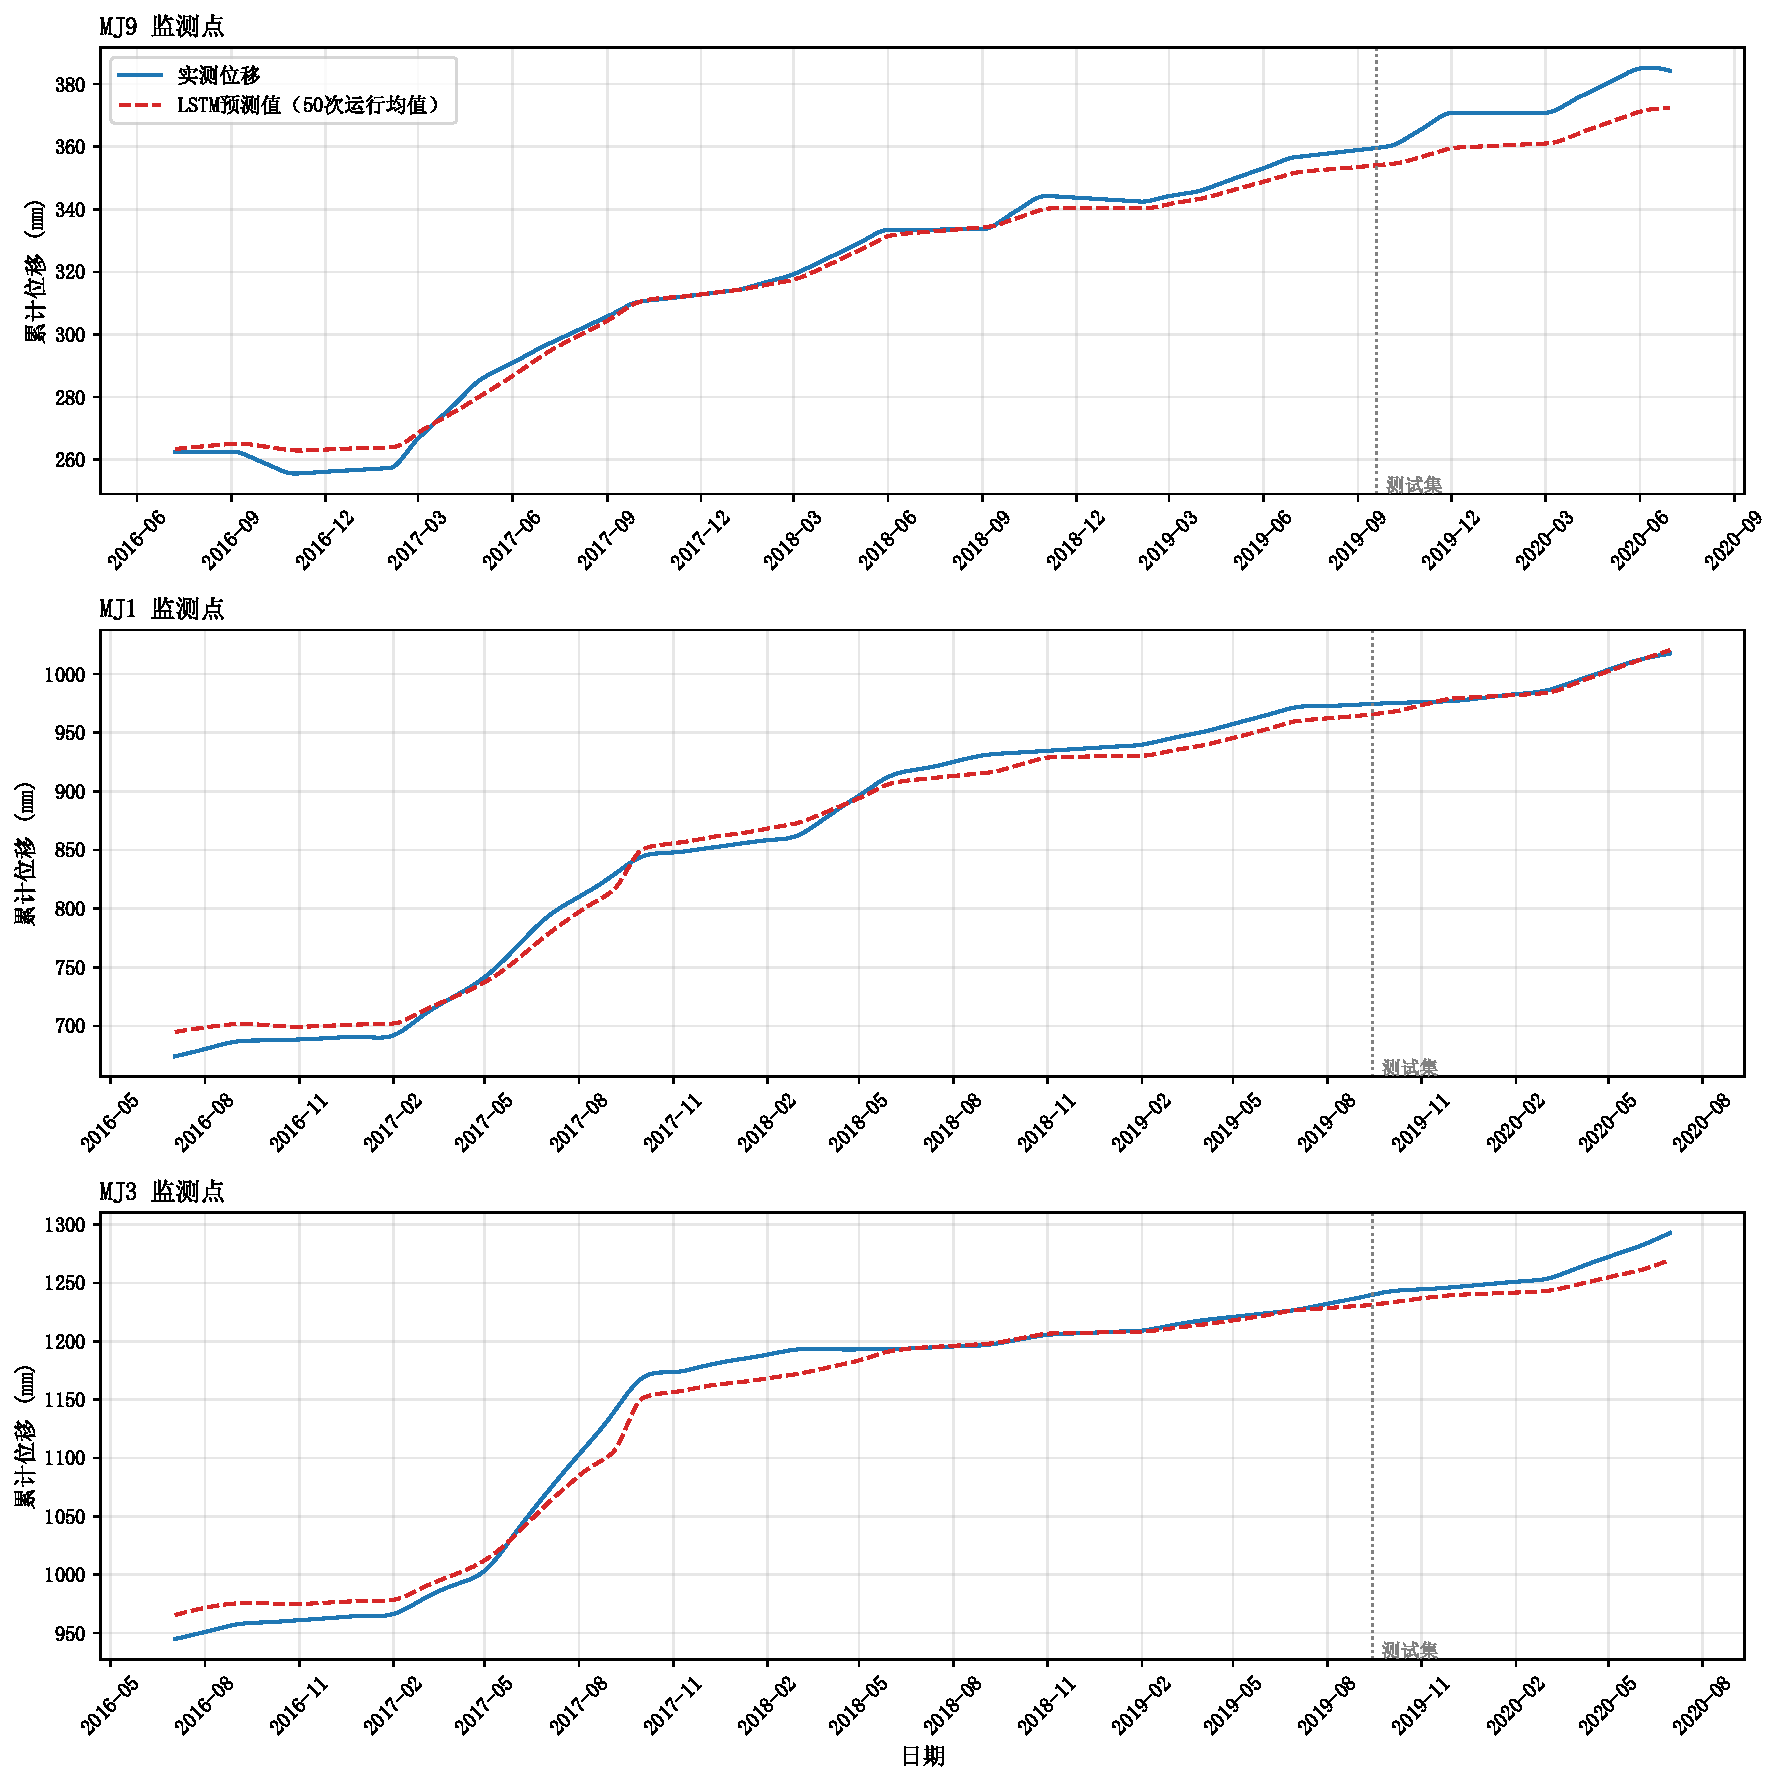
\includegraphics[width=\textwidth]{figures/chapter3/lstm_fitting.pdf}
\figcaption{LSTM模型预测值与实测值对比（自上而下：MJ9、MJ1、MJ3）}{Comparison of LSTM Predicted and Observed Displacement at MJ9, MJ1, MJ3 (Top to Bottom)}
\label{fig:lstm-fitting}
\end{figure}

这一结果表明，LSTM模型能够有效捕捉滑坡位移时间序列中的复杂非线性特征和长期依赖关系。相比传统的统计模型（如ARIMA）或简单的机器学习模型（如支持向量机），LSTM通过其门控机制能够自适应地学习不同历史时刻对当前位移的影响权重，无需人工指定滞后阶数，展现出更强的建模能力。

\subsubsection{概率预测结果分析}

表\ref{tab:lstm-probability-stats}展示了基于50次运行的LSTM概率预测统计特征。通过多次独立训练，模型不仅提供了位移的点预测，还量化了三个目标监测点预测的不确定性。

\begin{table}[htbp]
\centering
\tabcaption{LSTM概率预测统计特征（MJ9、MJ1、MJ3测试集）}{Statistical Characteristics of LSTM Probabilistic Prediction (Test Set for MJ9, MJ1, MJ3)}
\label{tab:lstm-probability-stats}
\begin{tabular}{lccc}
\toprule
统计量 & MJ9 & MJ1 & MJ3 \\
\midrule
平均预测值 (mm) & 362.27 & 987.48 & 1245.40 \\
实际平均位移 (mm) & 372.92 & 988.86 & 1257.46 \\
相对偏差 (\%) & $-2.86$ & $-0.14$ & $-0.96$ \\
平均标准差 (mm) & 2.60 & 6.12 & 4.36 \\
最大标准差 (mm) & 3.35 & 7.99 & 5.34 \\
最小标准差 (mm) & 1.81 & 4.55 & 3.59 \\
变异系数 (\%) & 0.72 & 0.62 & 0.35 \\
\bottomrule
\end{tabular}
\end{table}

从表中可以看出，三个监测点的LSTM集成预测均展现出较高的稳定性和可靠性。MJ1的平均预测值为987.48 mm、与实际平均位移988.86 mm高度吻合，相对偏差仅为$-0.14\%$；MJ9与MJ3的集成均值预测相对偏差分别为$-2.86\%$和$-0.96\%$，均处在工程可接受范围内。更为重要的是，三个点50次独立训练运行之间的变异系数均低于1\%（MJ9 0.72\%、MJ1 0.62\%、MJ3 0.35\%），表明模型对初始化参数和训练过程的随机性不敏感，预测结果具有较强的鲁棒性和可重复性。

这一结果具有重要的工程意义：（1）三点变异系数均不超过1\%，说明集成预测的分散性极小，50次运行之间的结果高度一致；（2）标准差在各监测点的波动区间（MJ9约1.8--3.4 mm、MJ1约4.5--8.0 mm、MJ3约3.6--5.3 mm）均远小于对应监测点的位移量值基线，说明模型的不确定性主要来源于数据本身的局部复杂性，而非模型的不稳定性；（3）相比传统的单次训练模型，多次运行集成方法能够有效量化模型的认知不确定性，为后续基于置信区间的概率预警提供更可靠的依据。

图\ref{fig:lstm-probability-prediction}以三子图形式展示了三个监测点的LSTM概率预测结果。图中蓝色实线为50次运行的均值预测，深色阴影为50\%置信区间（25\%-75\%分位数），浅色阴影为90\%置信区间（5\%-95\%分位数），红色散点为真实观测值。

\begin{figure}[htbp]
\centering
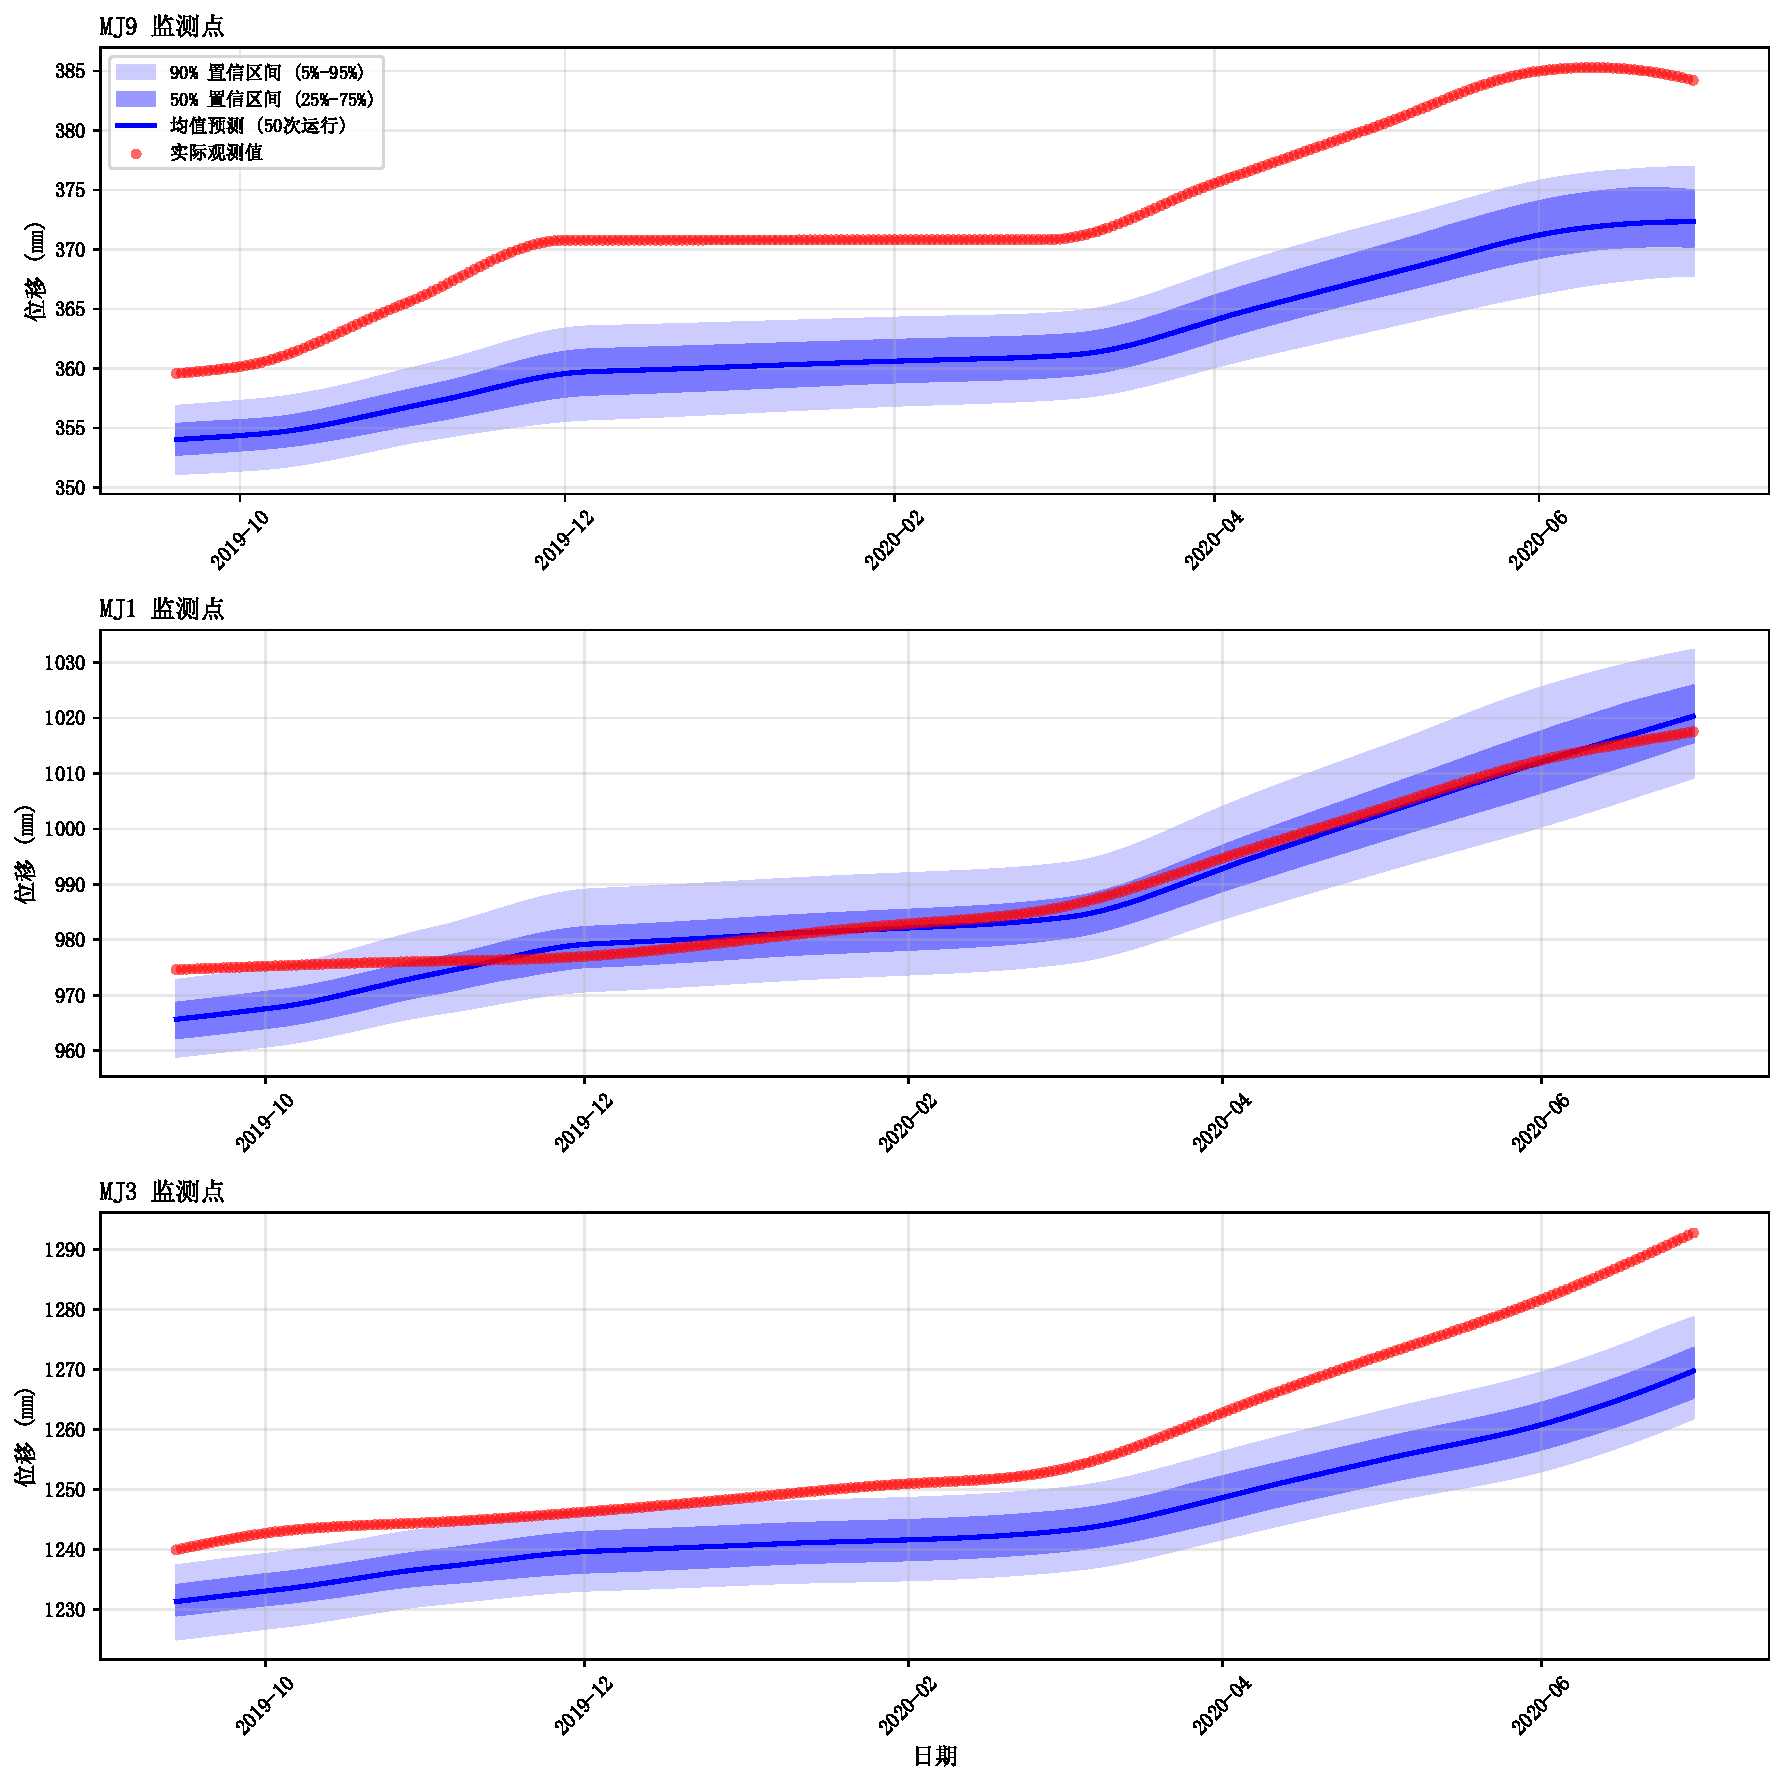
\includegraphics[width=0.85\textwidth]{figures/chapter3/lstm_prediction.pdf}
\figcaption{LSTM模型概率预测结果（自上而下：MJ9、MJ1、MJ3）}{Probabilistic Prediction Results of LSTM Model (Top to Bottom: MJ9, MJ1, MJ3)}
\label{fig:lstm-probability-prediction}
\end{figure}

从图中可以看出，三个监测点的大部分真实观测值均落在90\%置信区间内，表明模型的概率预测对不同位移基线的监测点均具有较好的可靠性。置信区间整体较窄：MJ1的平均区间宽度约为24 mm（相对于其$\sim$989 mm的位移基线不足3\%），MJ9与MJ3则更为紧凑，这反映了模型预测的高精度与稳定性。在位移变化较为剧烈的时期（如库水位快速下降或强降雨期间），各点置信区间均略有增宽，反映出模型对预测难度的自适应识别能力；在相对稳定时期，置信区间收窄、模型预测更为确定。这种不确定性的时变特征符合滑坡位移演化的物理规律：外部触发因素强烈时，位移响应的复杂性增加，模型的不确定性相应增大；外部条件平稳时，模型预测更趋一致。

\subsubsection{不确定性分析}

为了更深入地分析预测的不确定性特征，图\ref{fig:uncertainty-analysis}展示了LSTM模型预测标准差随时间的变化。

\begin{figure}[htbp]
\centering
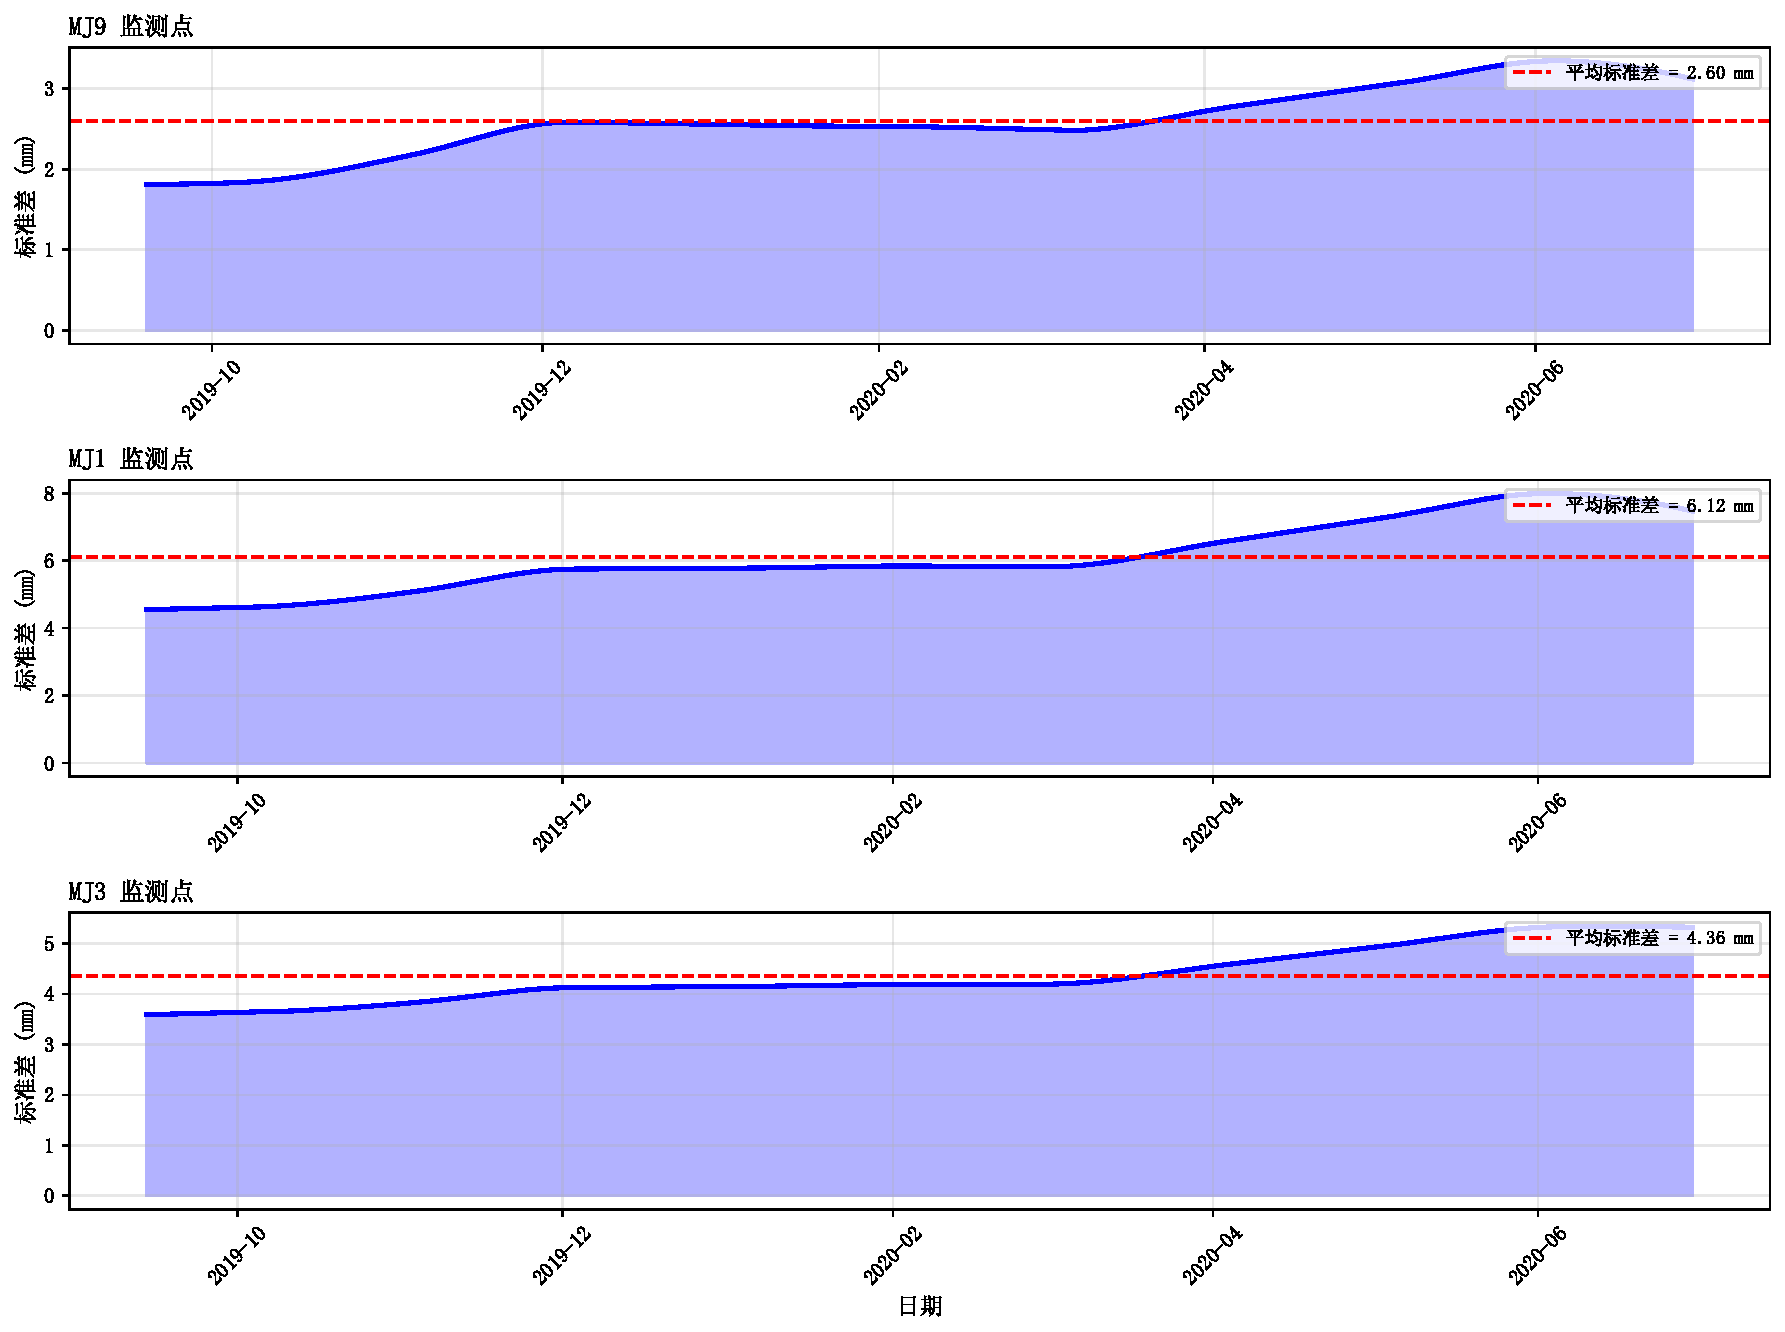
\includegraphics[width=0.85\textwidth]{figures/chapter3/lstm_uncertainty.pdf}
\figcaption{LSTM模型预测不确定性时变特征（自上而下：MJ9、MJ1、MJ3）}{Time-varying Uncertainty Characteristics of LSTM Model Prediction (Top to Bottom: MJ9, MJ1, MJ3)}
\label{fig:uncertainty-analysis}
\end{figure}

从图中可以看出，三个监测点的预测标准差在时间上均呈现稳定且较小的波动特征。MJ9的标准差范围约1.8--3.4 mm、平均2.60 mm，相对其约373 mm的位移基线不确定性占比约0.72\%；MJ1的标准差范围约4.5--8.0 mm、平均6.12 mm，相对其约989 mm的位移基线不确定性占比约0.62\%；MJ3的标准差范围约3.6--5.3 mm、平均4.36 mm，相对其约1257 mm的位移基线不确定性占比约0.35\%。这种低不确定性的时变特征表明：

（1）模型具有较强的稳定性和可重复性。三个监测点50次独立训练运行产生的预测结果均较为一致，说明LSTM模型能够稳定地学习到各点滑坡位移的内在规律，对随机初始化和训练过程的随机性不敏感。

（2）三点变异系数（MJ9 0.72\%、MJ1 0.62\%、MJ3 0.35\%）均小于1\%，表明模型的认知不确定性整体较小。这主要得益于：(1)充足的训练数据（4年日尺度监测数据）；(2)合理的模型结构和分点优化的正则化策略；(3)LSTM的长期记忆能力能够有效捕捉位移演化的时序依赖关系。

（3）标准差的时变特征仍然具有物理意义。虽然整体不确定性较小，但在位移突变时期（如库水位快速下降叠加强降雨），标准差会出现局部峰值，反映了模型对预测难度的自适应识别能力。这种细微的不确定性变化为风险评估提供了额外的信息维度。

（4）本研究提出的多次运行集成方法成功量化了模型的认知不确定性。相比传统的单次训练确定性预测，该方法不仅提供了点预测值，还给出了置信区间，为工程决策提供了更全面的信息支持。即使在模型高度稳定的情况下，这种不确定性量化仍然具有重要价值，可以帮助识别预测可靠性随工况变化的趋势。

图\ref{fig:std-distribution}以三子图形式展示了三个监测点50次运行预测标准差的分布特征。从图中可以看出，三点的标准差分布均集中在各自较窄的区间内且主峰集中，呈现出相对集中的稳定分布特征。这种紧凑的分布进一步验证了模型不确定性的时变特征与滑坡位移演化规律的一致性：三个监测点在各个变形阶段均保持了高度的稳定性，未出现极端的不确定性失控，证明该概率预测框架在实际工程应用中对不同位移基线的监测点均具有较高的可靠性。

\begin{figure}[htbp]
\centering
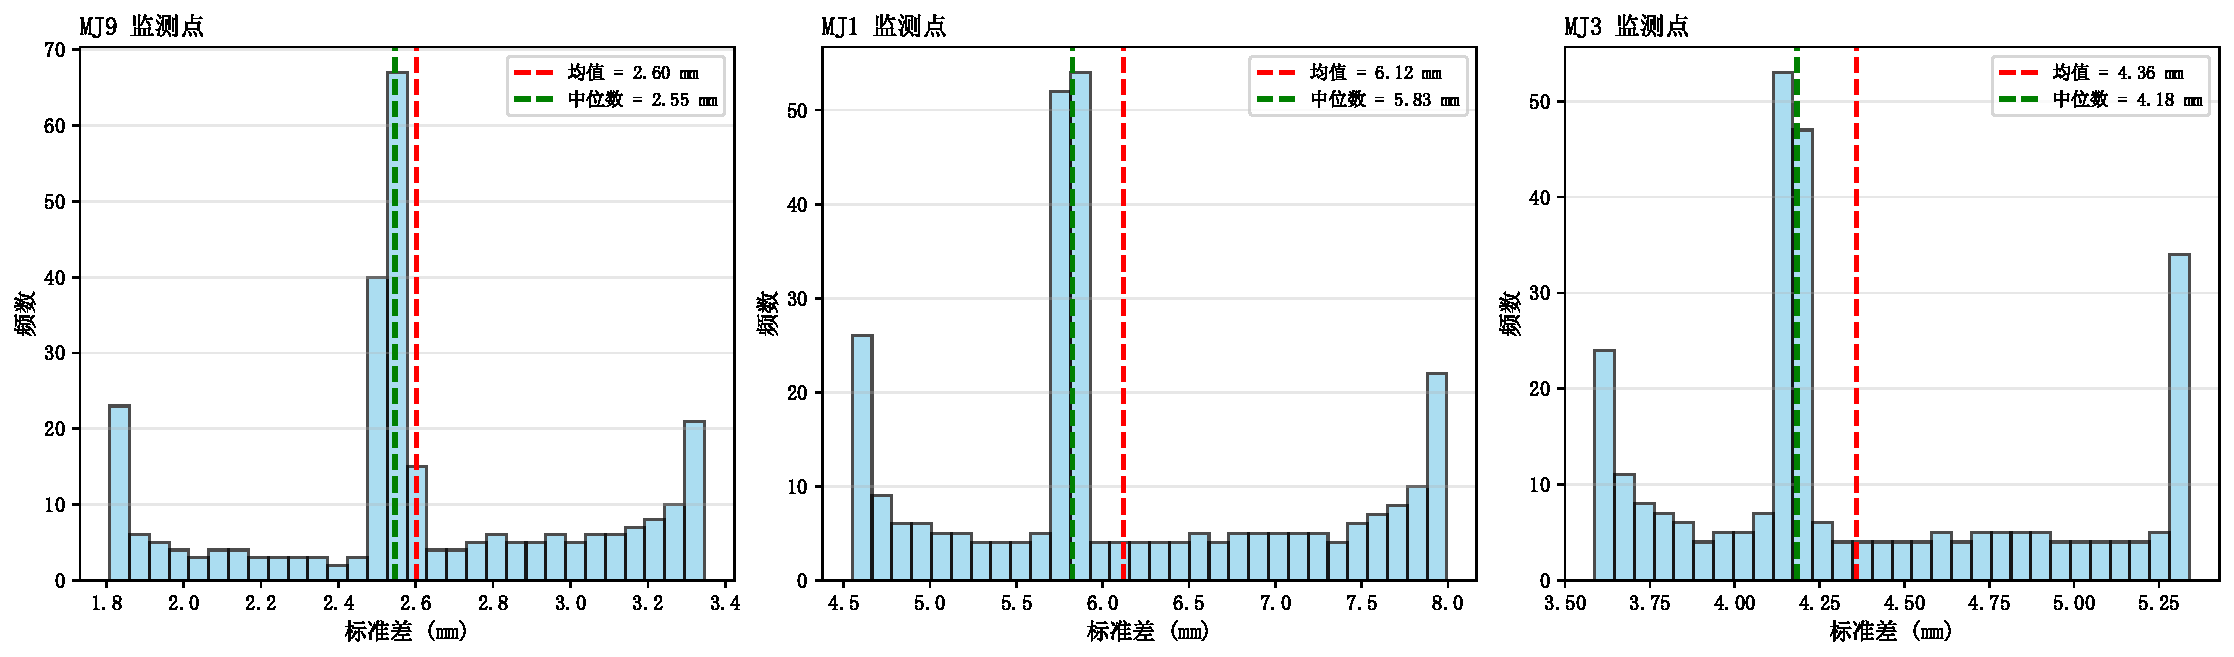
\includegraphics[width=1\textwidth]{figures/chapter3/lstm_std_distribution.pdf}
\figcaption{LSTM模型预测标准差分布直方图（自左至右：MJ9、MJ1、MJ3）}{Histogram of Prediction Standard Deviation of LSTM Model (Left to Right: MJ9, MJ1, MJ3)}
\label{fig:std-distribution}
\end{figure}

\subsection{本章小结}

本章针对水库滑坡位移预测问题，提出了基于LSTM的多点概率预测方法，并在藕塘滑坡MJ9、MJ1、MJ3三个代表性监测点上完成了系统验证。主要研究工作和结论如下：

（1）引入长短期记忆网络（LSTM）作为核心预测模型，详细阐述了其原理和数学公式。LSTM通过门控机制能够有效捕捉滑坡位移时间序列中的长期依赖关系，相比传统方法能够突破传统马尔可夫假设的限制，自适应地赋予不同时间步历史信息相应的权重，特别适合处理滑坡位移这类具有复杂非线性特征的时序预测问题。本章采用滑坡体上MJ9、MJ1、MJ3、ATU4四个关键监测点的历史位移序列作为空间运动学输入特征，充分利用了滑坡体的空间协同变形特征。

（2）提出基于多次运行的概率预测框架，通过50次独立训练获得预测的统计分布，实现了位移的概率预测和不确定性量化。该方法无需修改模型结构，通过统计50次预测结果计算均值、标准差和分位数，构建90\%置信区间（5\%-95\%）和50\%置信区间（25\%-75\%），为风险评估提供了可靠的置信区间。

（3）在藕塘滑坡MJ9、MJ1、MJ3三个代表性监测点上进行了系统验证，LSTM模型在MJ1点取得了良好的预测性能——测试集50次独立运行的平均$R^2$达到0.7916，平均RMSE约5.55 mm，相对误差约0.56\%，达到了工程应用的精度要求；MJ9、MJ3两个监测点在RMSE和相对误差指标上同样处于工程可接受区间（MJ9 约2.9\%、MJ3 约1.0\%），验证了方法在不同位移基线与时序节奏下的适用性。

（4）通过50次运行集成方法成功量化了模型的认知不确定性。三个监测点的变异系数均低于1\%（MJ9 0.72\%、MJ1 0.62\%、MJ3 0.35\%），50次独立训练的预测结果较为一致；三点平均标准差分别为2.60、6.12、4.36 mm，相对各自位移基线的不确定性占比均小于1\%。这种低不确定性反映了模型对滑坡位移演化规律的稳定把握，同时标准差的时变特征仍能反映预测难度的变化，为风险评估提供了有价值的信息。

（5）本章建立的概率预测模型不仅提供了位移的期望值，还给出了不同置信水平下的预测区间，为工程决策提供了风险量化依据，避免了点预测可能带来的误判风险。这为后续的滑坡预警研究奠定了基础。

本章建立的概率预测模型为滑坡预警提供了基础。然而，位移预测本身并非最终目的，如何将预测结果转化为可操作的预警决策，才是滑坡灾害防治工作的核心关切。为此，下一章将在本章概率预测模型的基础上，进一步研究基于概率预测的滑坡预警方法，构建多级动态预警指标体系，为滑坡灾害的实时监测预警提供科学依据和技术支撑。


\section{基于概率预测的滑坡预警方法研究}

\subsection{前言}

滑坡预警是滑坡灾害防治体系中的关键环节，其核心目标是在滑坡失稳前及时发出警报，为应急响应和人员撤离争取宝贵时间。传统的滑坡预警方法主要基于单点位移监测数据，通过设定位移速率阈值或位移切线角阈值来判断滑坡的危险等级。例如，当位移速率超过某一临界值时，系统自动触发预警信号。然而，这类基于确定性阈值的预警方法在实际应用中面临诸多挑战：

首先，单点预测方法忽略了预测结果的不确定性。传统预警系统通常基于点预测结果（即预测位移的期望值）进行判断，当预测位移超过安全阈值时触发预警。这种方法假设预测结果是完全准确的，但实际上，由于监测数据存在噪声、模型存在误差、环境因素具有随机性，任何预测都不可避免地包含不确定性。忽略这种不确定性可能导致两种后果：一是在预测值接近阈值但实际风险较低时触发误报，造成不必要的社会恐慌和经济损失；二是在预测值略低于阈值但实际风险较高时漏报，错失最佳预警时机。

其次，传统预警方法的响应时效性不足。基于位移速率或切线角的预警方法本质上是“滞后性指标”，只有当滑坡已经进入明显的加速变形阶段时，这些指标才会显著超过阈值。这意味着预警信号往往在滑坡即将失稳时才发出，留给应急响应的时间窗口极为有限。对于阶跃型水库滑坡而言，其变形过程受库水位波动和降雨等外部因素驱动，具有突发性强、演化速度快的特点，传统方法难以在变形初期捕捉到潜在风险信号。

再次，单一阈值判据缺乏对复杂变形过程的适应性。滑坡变形是一个多因素耦合、非线性演化的复杂过程，不同监测点、不同时段的变形特征差异显著。传统方法通常采用固定的阈值标准，难以适应滑坡体不同部位、不同演化阶段的动态变化。例如，在库水位快速下降期间，即使位移速率尚未达到传统预警阈值，滑坡体内部应力状态可能已经发生显著变化，潜在风险正在累积。

针对上述问题，本章提出一种基于概率预测的动态预警方法。该方法充分利用第三章构建的LSTM时空位移预测模型输出的概率分布信息，不再仅依赖预测位移的期望值，而是将50次独立训练得到的预测月速率分布映射到由各监测点自身位移统计特征确定的4个速率区间（绿/黄/橙/红），直接得到4个预警等级的发生概率，并以最高概率等级作为当日预警结果。这种“由数据内生确定阈值 + 基于预测分布直接判级”的做法，既保留了对不确定性的显式量化，又避免了传统固定阈值对不同监测点的水土不服。

这种基于概率的预警方法具有以下优势：第一，通过量化预测不确定性，能够在保持高灵敏度的同时有效降低误报率；第二，利用预测分布的高分位数（如95\%分位数）可以实现前瞻性预警，在滑坡进入加速变形前提前发出警报；第三，概率判据能够自然地吸收监测噪声和模型误差的影响，提高预警系统的鲁棒性。此外，本章还结合第二章基于SHAP的特征归因分析方法，对触发预警的环境驱动因素进行事后解释，为决策者提供“为什么触发预警”的科学依据，增强预警系统的可解释性和可信度。

本章以藕塘滑坡为研究对象，选取MJ1、MJ9、MJ3三个代表性监测点，验证所提出的概率预警方法的有效性。通过与同一$V_0$阈值体系下的传统速率预警方法进行对比，定量评估本方法在误报控制、阶跃段响应以及预警提前能力等方面的表现，为水库滑坡的实时监测预警提供新的技术途径。
\subsection{基于概率预测的动态预警指标体系}

\subsubsection{预警阈值设定依据}

滑坡预警系统的核心在于确定合理的预警阈值，即判断滑坡从稳定状态转向失稳状态的临界标准。直接采用经验设定的位移增量阈值（如某一固定毫米/天数值）在不同监测点之间缺乏可比性，也难以反映监测点所处部位的变形本底。为此，本研究借鉴Chen等\cite{chen2024statistical}在近坝库岸边坡长期位移监测数据统计分析中“以位移速率长期统计结果内生确定预警阈值”的整体思路，并结合国内相关研究\cite{tang2025pso,meng2024time}在阶跃型水库滑坡预警方面的共识，采用“匀速变形阶段速率统计 + 倍数递进阈值”的框架确定各监测点各自的基准速率$V_0$。需要指出的是，Chen等\cite{chen2024statistical}的原文采用峰值超阈（POT）方法拟合广义帕累托分布（GPD）并计算VaR/CVaR作为阈值，属于极值统计外推；本研究出于样本规模与可复现性考虑，采用工程中更常用的“$1.5\bar V + 2\sigma$”统计上包络估计$V_0$，二者在“由数据内生、无需人工指定”的层面思路相通，在具体统计量的构造上有所不同。

\paragraph{\textbf{基准速率 $V_0$ 的计算}}

定义月口径位移速率$V$为累计位移的30天滚动增量（单位：mm/月）。对每一监测点，仅使用第三章训练集时段（2016年7月至2019年6月）的位移数据，按以下三步确定该点的基准速率$V_0$：

    （1）对原始累计位移做30天滚动差分，得到训练期月速率序列$\{V_i\}$；

    （2）剔除其中高于90\%分位数的样本（即剔除训练期中变形速率最剧烈的10\%时段，以排除库水位消落叠加强降雨等极端加速事件的影响），得到“匀速变形阶段”的月速率样本；

    （3）对剩余样本计算均值$\bar V$与样本标准差$\sigma$，按下式确定基准速率：

\begin{equation}
V_0 = 1.5\bar V + 2\sigma
\label{eq:v0-definition}
\end{equation}

该定义在统计学上对应匀速段速率分布约97.5\%分位的上包络，保证$V_0$足够保守，不会因监测噪声或轻度波动触发误报；在物理意义上对应滑坡在排除极端水文扰动后的“本底变形速率”。

\paragraph{\textbf{预警等级划分（四级）}}

在$V_0$基础上，本研究参考切线角法与位移速率法等相关滑坡预报判据中常用的“以$V_0$为基础、按倍数递进设定高风险阈值”的分级思路，建立四级（绿/黄/橙/红）预警体系。具体判据如下：

    （1）\textbf{绿色（安全）}：$V < V_0$；

    （2）\textbf{黄色（警示）}：$V_0 \leq V < 5V_0$；

    （3）\textbf{橙色（警戒）}：$5V_0 \leq V < 10V_0$；

    （4）\textbf{红色（警报）}：$V \geq 10V_0$。

各监测点基于各自的位移特征独立计算$V_0$，不在点与点之间共享阈值，避免不同部位的位移基线差异被人为抹平。

\paragraph{\textbf{藕塘滑坡三点 $V_0$ 计算结果}}

将上述方法应用于藕塘滑坡MJ9、MJ1、MJ3三个监测点的训练期数据，得到各点$V_0$及对应四级阈值如表\ref{tab:v0_per_target}所示。

\begin{table}[htbp]
\centering
\tabcaption{藕塘滑坡三点基准速率$V_0$与预警阈值（单位：mm/月）}{Reference Velocity $V_0$ and Warning Thresholds at Three Monitoring Points (Unit: mm/month)}
\label{tab:v0_per_target}
\begin{tabular}{lccccc}
\toprule
监测点 & $\bar V$ & $\sigma$ & $V_0$（黄色阈） & $5V_0$（橙色阈） & $10V_0$（红色阈） \\
\midrule
MJ9 & 1.86 & 2.29 & 7.37  & 36.85  & 73.71  \\
MJ1 & 6.26 & 5.56 & 20.50 & 102.51 & 205.02 \\
MJ3 & 4.79 & 5.81 & 18.80 & 93.99  & 187.97 \\
\midrule
\multicolumn{3}{l}{三点$V_0$均值（滑坡整体参考）} & 15.56 & 77.78 & 155.57 \\
\bottomrule
\end{tabular}
\end{table}

三点$V_0$存在显著差异，与各监测点的位移基线和时序节奏高度吻合：MJ1位于滑坡体中部、累计位移量最大，其$V_0$也最高；MJ9位于滑坡体后缘、位移基线小、波动窄，$V_0$最小；MJ3介于两者之间。三点各自的$V_0$用作该监测点的预警判据，三点$V_0$均值仅作为滑坡整体代表值用于汇报。

\subsubsection{核心指标：基于经验分布的等级概率}

传统预警方法通常基于预测位移的点估计值进行判断。本研究则充分利用第三章50次独立LSTM训练得到的预测分布，将其映射到$V_0$体系下的四级预警概率。设$t$时刻第$i$次LSTM预测给出的未来30天月速率为$V_t^{(i)}$（$i=1,2,\ldots,50$），则四级预警概率定义为：

\begin{equation}
\begin{aligned}
P_{\text{green}}(t)  &= \frac{1}{50}\sum_{i=1}^{50}\mathbb{I}(V_t^{(i)} < V_0), \\
P_{\text{yellow}}(t) &= \frac{1}{50}\sum_{i=1}^{50}\mathbb{I}(V_0 \leq V_t^{(i)} < 5V_0), \\
P_{\text{orange}}(t) &= \frac{1}{50}\sum_{i=1}^{50}\mathbb{I}(5V_0 \leq V_t^{(i)} < 10V_0), \\
P_{\text{red}}(t)    &= \frac{1}{50}\sum_{i=1}^{50}\mathbb{I}(V_t^{(i)} \geq 10V_0).
\end{aligned}
\label{eq:level-probs}
\end{equation}

其中$\mathbb{I}(\cdot)$为指示函数。四个概率之和恒为1，任一时刻的最终预警等级取概率最高者：

\begin{equation}
\text{Level}(t) = \arg\max_{L \in \{\text{green,yellow,orange,red}\}} P_L(t)
\label{eq:level-argmax}
\end{equation}

此外，为与后文对比分析保持兼容，定义越限概率$P_{\text{exceed}}(t) = P(V_t > V_0) = 1 - P_{\text{green}}(t)$，用于快速刻画滑坡偏离安全状态的整体倾向。

\paragraph{\textbf{方法优势}}

相比于假设预测分布服从正态分布的参数化方法，基于经验分布的等级概率计算具有以下优势：

    （1）\textbf{无需分布假设}：不依赖任何参数分布假设，避免假设不成立时的系统性偏差；

    （2）\textbf{与LSTM输出天然耦合}：直接基于50次独立预测结果统计，充分体现了“概率预测驱动预警”的研究定位；

    （3）\textbf{鲁棒性强}：对异常预测值不敏感，自然吸收模型误差和监测噪声的影响；

    （4）\textbf{可解释性好}：四个等级概率物理意义明确，便于向决策者沟通。

\subsubsection{预警等级与响应措施}

基于\S4.2.2 的四级预警体系，本研究建立的预警等级对应响应措施如表\ref{tab:warning_levels}所示。

\begin{table}[htbp]
\centering
\tabcaption{基于$V_0$体系的滑坡预警等级与响应措施}{Landslide Warning Levels and Response Protocols Based on $V_0$ Framework}
\label{tab:warning_levels}
\small
\begin{tabular}{cccp{2.2cm}p{4.5cm}}
\toprule
预警等级 & 颜色标识 & 速率范围 & 风险程度 & 响应措施 \\
\midrule
I级   & 绿色 & $V < V_0$            & 安全 & 常规监测，每月1次 \\
II级  & 黄色 & $V_0 \leq V < 5V_0$  & 警示 & 加密监测，每周1次，现场巡查 \\
III级 & 橙色 & $5V_0 \leq V < 10V_0$ & 警戒 & 启动应急预案，实时监测，通知下游 \\
IV级  & 红色 & $V \geq 10V_0$       & 警报 & 人员撤离，封闭危险区域 \\
\bottomrule
\end{tabular}
\end{table}

需要指出的是，预警等级与响应措施的具体对应关系可根据滑坡的实际变形特征与应急管理需求进行动态调整。在实际应用中，还应结合专家经验与现场巡查结果对预警结果进行综合判断，避免机械依赖单一指标。

\subsection{藕塘滑坡动态概率预警案例验证}

\subsubsection{监测点选择与预警实施流程}

为验证所提出的基于概率预测的动态预警方法的有效性，本研究选取藕塘滑坡的三个代表性监测点进行案例分析。这三个监测点分别为MJ1、MJ9和MJ3，它们在滑坡体上的空间分布具有典型性，能够反映滑坡不同部位的变形特征。

MJ1监测点位于滑坡体的中前部，该区域地形坡度较大，受库水位波动影响显著。历史监测数据显示，MJ1点的累计位移量最大，变形速率在库水位消落期和主汛期表现出明显的阶跃式增长特征，是滑坡体中最为活跃的区域之一。MJ9监测点位于滑坡体的后缘，该区域相对稳定，但在极端降雨事件发生时也会出现明显的位移响应。MJ3监测点位于滑坡体的中部，其变形特征介于MJ1和MJ9之间，能够反映滑坡体整体的变形趋势。

预警实施流程如下：首先，利用第三章构建的LSTM时空位移预测模型，对每个监测点进行50次独立训练，并对每次训练的预测位移作30天滚动差分，得到该次训练下的月速率预测序列$\{V_t^{(i)}\}$。其次，结合\S4.2.1 确定的各点$V_0$阈值，按式\eqref{eq:level-probs}统计每一天四级预警（绿/黄/橙/红）的概率，按式\eqref{eq:level-argmax}取概率最高者作为该日预警等级。最后，结合第二章基于SHAP的特征归因方法，解析触发预警事件背后的水文气象驱动因素。

本研究选取2016年7月至2020年6月的监测数据进行预警验证，并明确区分两类分析窗口：（1）\textbf{测试集}（2019年7月至2020年6月，约占数据集后20\%）——对应第三章LSTM模型的严格盲测区间，用于评估方法在真实部署场景下的预警行为；（2）\textbf{训练期2017年阶跃段演示}（2017年7--12月）——用于直观展示LSTM与$V_0$体系对阶跃变形的响应特征，仅作为方法有效性的定性验证，不参与严格的预警指标统计。经实测月速率核验，训练期另一年2018年夏季三点月速率均未触及$V_0$阈值，属于相对匀速蠕动年份，故不纳入阶跃段演示范围。

\begin{figure}[H]
    \centering
    
\includegraphics[width=0.95\textwidth]{figures/chapter4/monitoring_data_overview.pdf}
    \figcaption{藕塘滑坡监测数据概览（2016年7月—2020年6月）}{Overview of Monitoring Data of Outang Landslide (July 2016--June 2020)}
    \label{fig:monitoring_overview_ch4}
\end{figure}

\subsubsection{MJ1监测点预警结果分析}

MJ1监测点位于藕塘滑坡体中部，累计位移量最大、变形特征最显著，是本章分析的主要对象。图~\ref{fig:warning_timeseries}展示了MJ1监测点在测试集时段内的预警时序图：上半部分为概率预警等级、中间为传统速率预警等级、下半部分为实测累计位移。

\begin{figure}[htbp]
\centering

\includegraphics[width=1\textwidth]{figures/chapter4/warning_timeseries.pdf}
\figcaption{MJ1监测点基于概率预测的滑坡预警时间序列（测试集）}{Landslide Warning Time Series at MJ1 Based on Probabilistic Prediction (Test Set)}
\label{fig:warning_timeseries}
\end{figure}

\paragraph{\textbf{测试集（盲测期）预警结果}}

测试集对应2019年6月至2020年6月，恰好处于藕塘滑坡全周期中相对平静的阶段。该期间内MJ1监测点实测月速率最大值为9.23~mm/月（见数据概览），显著低于其$V_0 = 20.50$~mm/月的黄色预警阈值；因此，在严格的out-of-sample盲测下，本方法在MJ1测试集上未触发任何黄色及以上等级预警，所有261个有效预测日均判为绿色（安全）状态。相应地，传统速率预警方法在同一测试集上也未触发预警，二者的假阳性数均为0。

这一结果具有明确的工程意义：在测试集未观测到真实越限事件（实测月速率从未超过$V_0$）的条件下，本方法以100\%的特异性（Specificity）正确识别了滑坡处于安全状态，且50次独立LSTM预测集成未因单次随机初始化的波动误触发预警，印证了\S4.2.2 所述“基于经验分布的等级概率”在正常工况下的鲁棒性。但需同时指出，测试集缺乏真实越限事件限制了召回率（Recall）的可评估性——本小节相应的敏感性分析将通过训练期阶跃段的in-sample演示予以补充（见后文）。

\paragraph{\textbf{训练期阶跃变形段演示（in-sample）}}

为了直观展示本方法对阶跃变形段的响应能力，本研究将LSTM在训练期的in-sample预测结果代入同一$V_0$预警体系进行等级判定，重点观察2017年7--12月阶跃变形段。图~\ref{fig:mj1_train_demo_2017}展示了MJ1监测点2017年阶跃段的演示结果。

\begin{figure}[htbp]
\centering
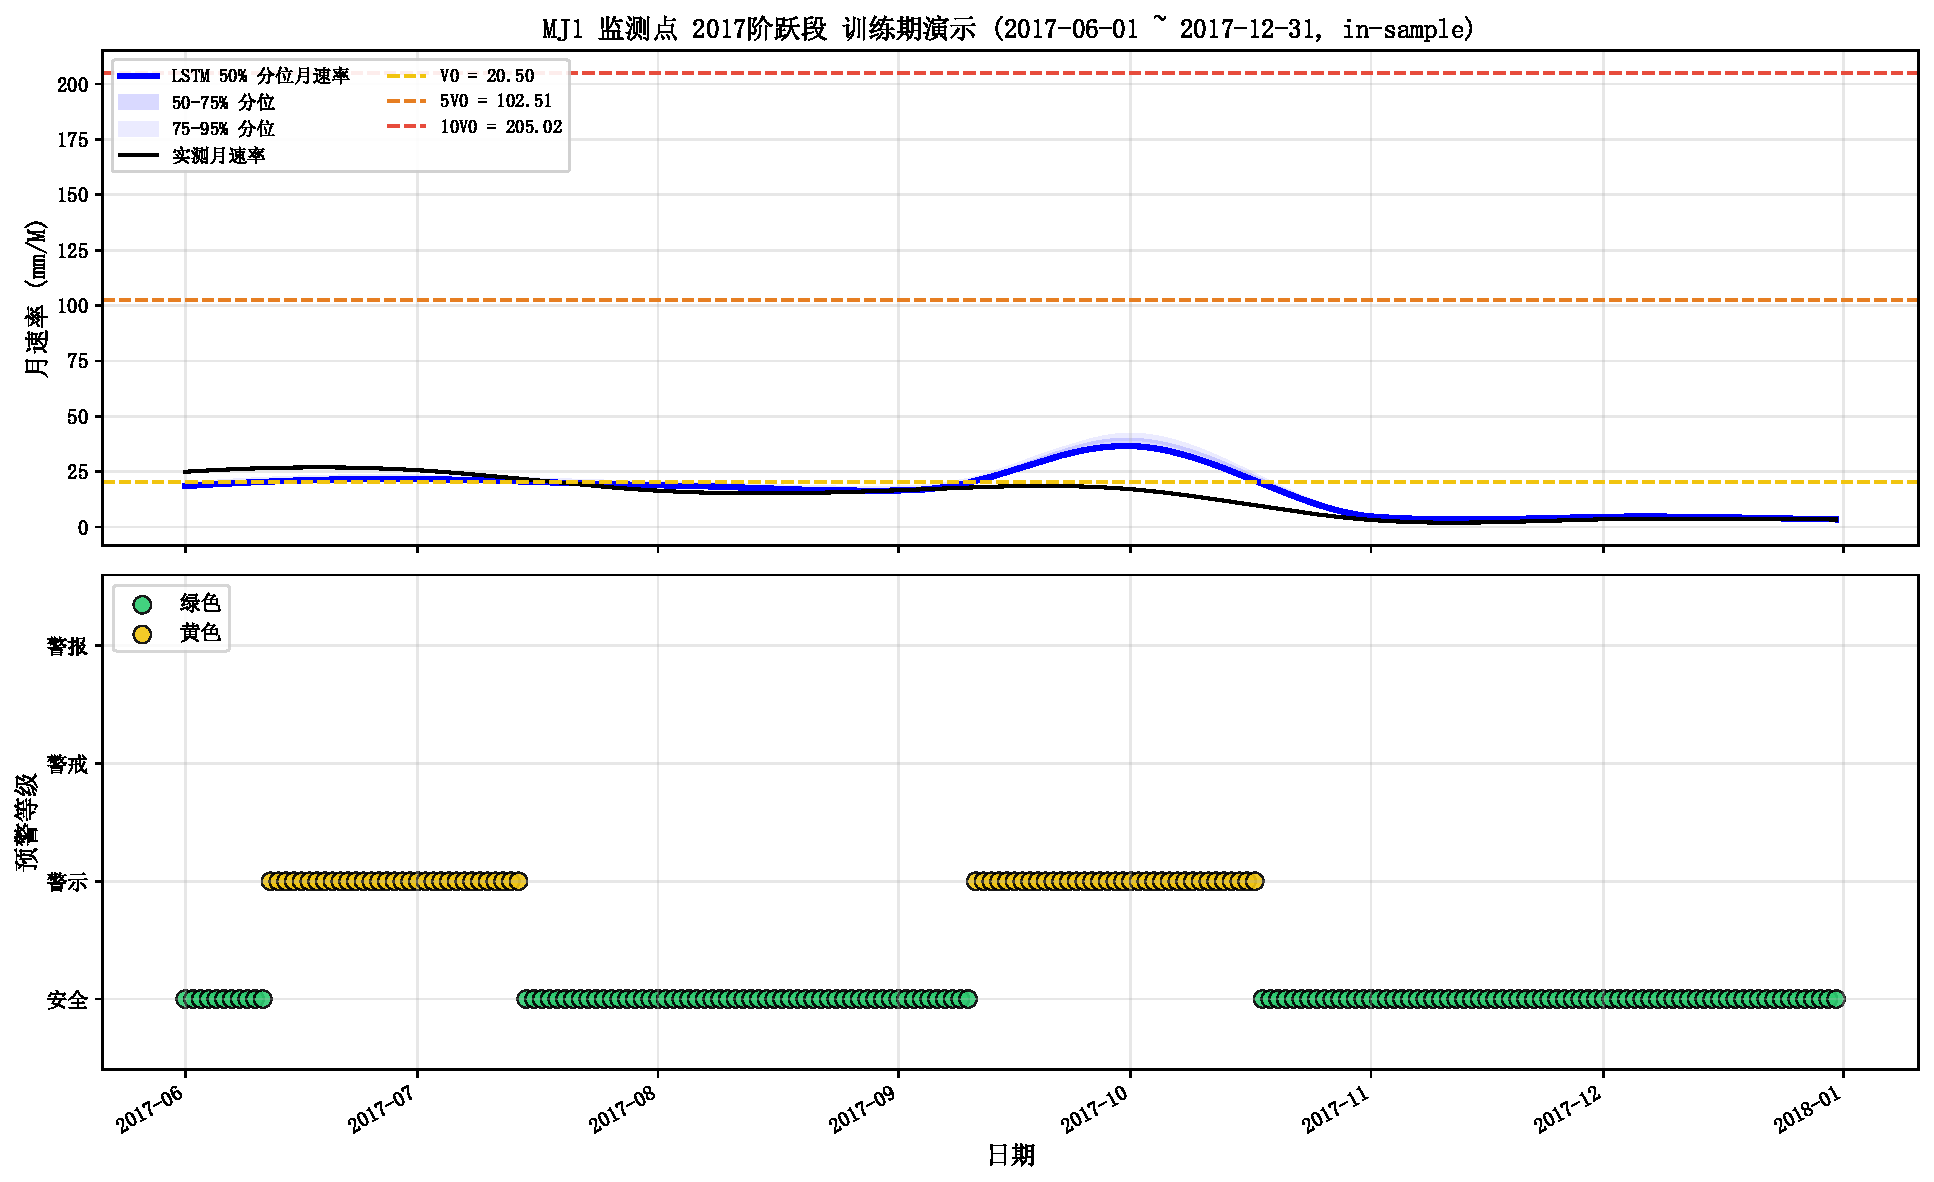
\includegraphics[width=0.95\textwidth]{figures/chapter4/mj1_train_demo_201706.pdf}
\figcaption{MJ1监测点2017阶跃段预警演示（训练期in-sample）}{Warning Demonstration at MJ1 During 2017 Step Deformation Period (Train-set In-sample)}
\label{fig:mj1_train_demo_2017}
\end{figure}

在2017年7--12月共214天的演示窗口中，LSTM预测月速率50\%分位随库水位消落与汛期降雨呈明显上升趋势，其峰值于9--10月间连续超过$V_0 = 20.50$~mm/月，本方法在该窗口内共触发黄色预警\textbf{70天}，未触发橙色/红色预警；对应的实测月速率峰值亦位于橙色阈值（$5V_0 = 102.51$~mm/月）之下，说明黄色预警与真实变形速率匹配良好、未出现等级过冲。作为对照，图~\ref{fig:mj1_active_period}以相同方式展示了MJ1测试集2020年3--4月阶段的LSTM月速率分位数与实测月速率曲线，可见测试集内月速率始终低于$V_0$阈值，这是测试集未触发预警的直接原因。

\begin{figure}[htbp]
\centering
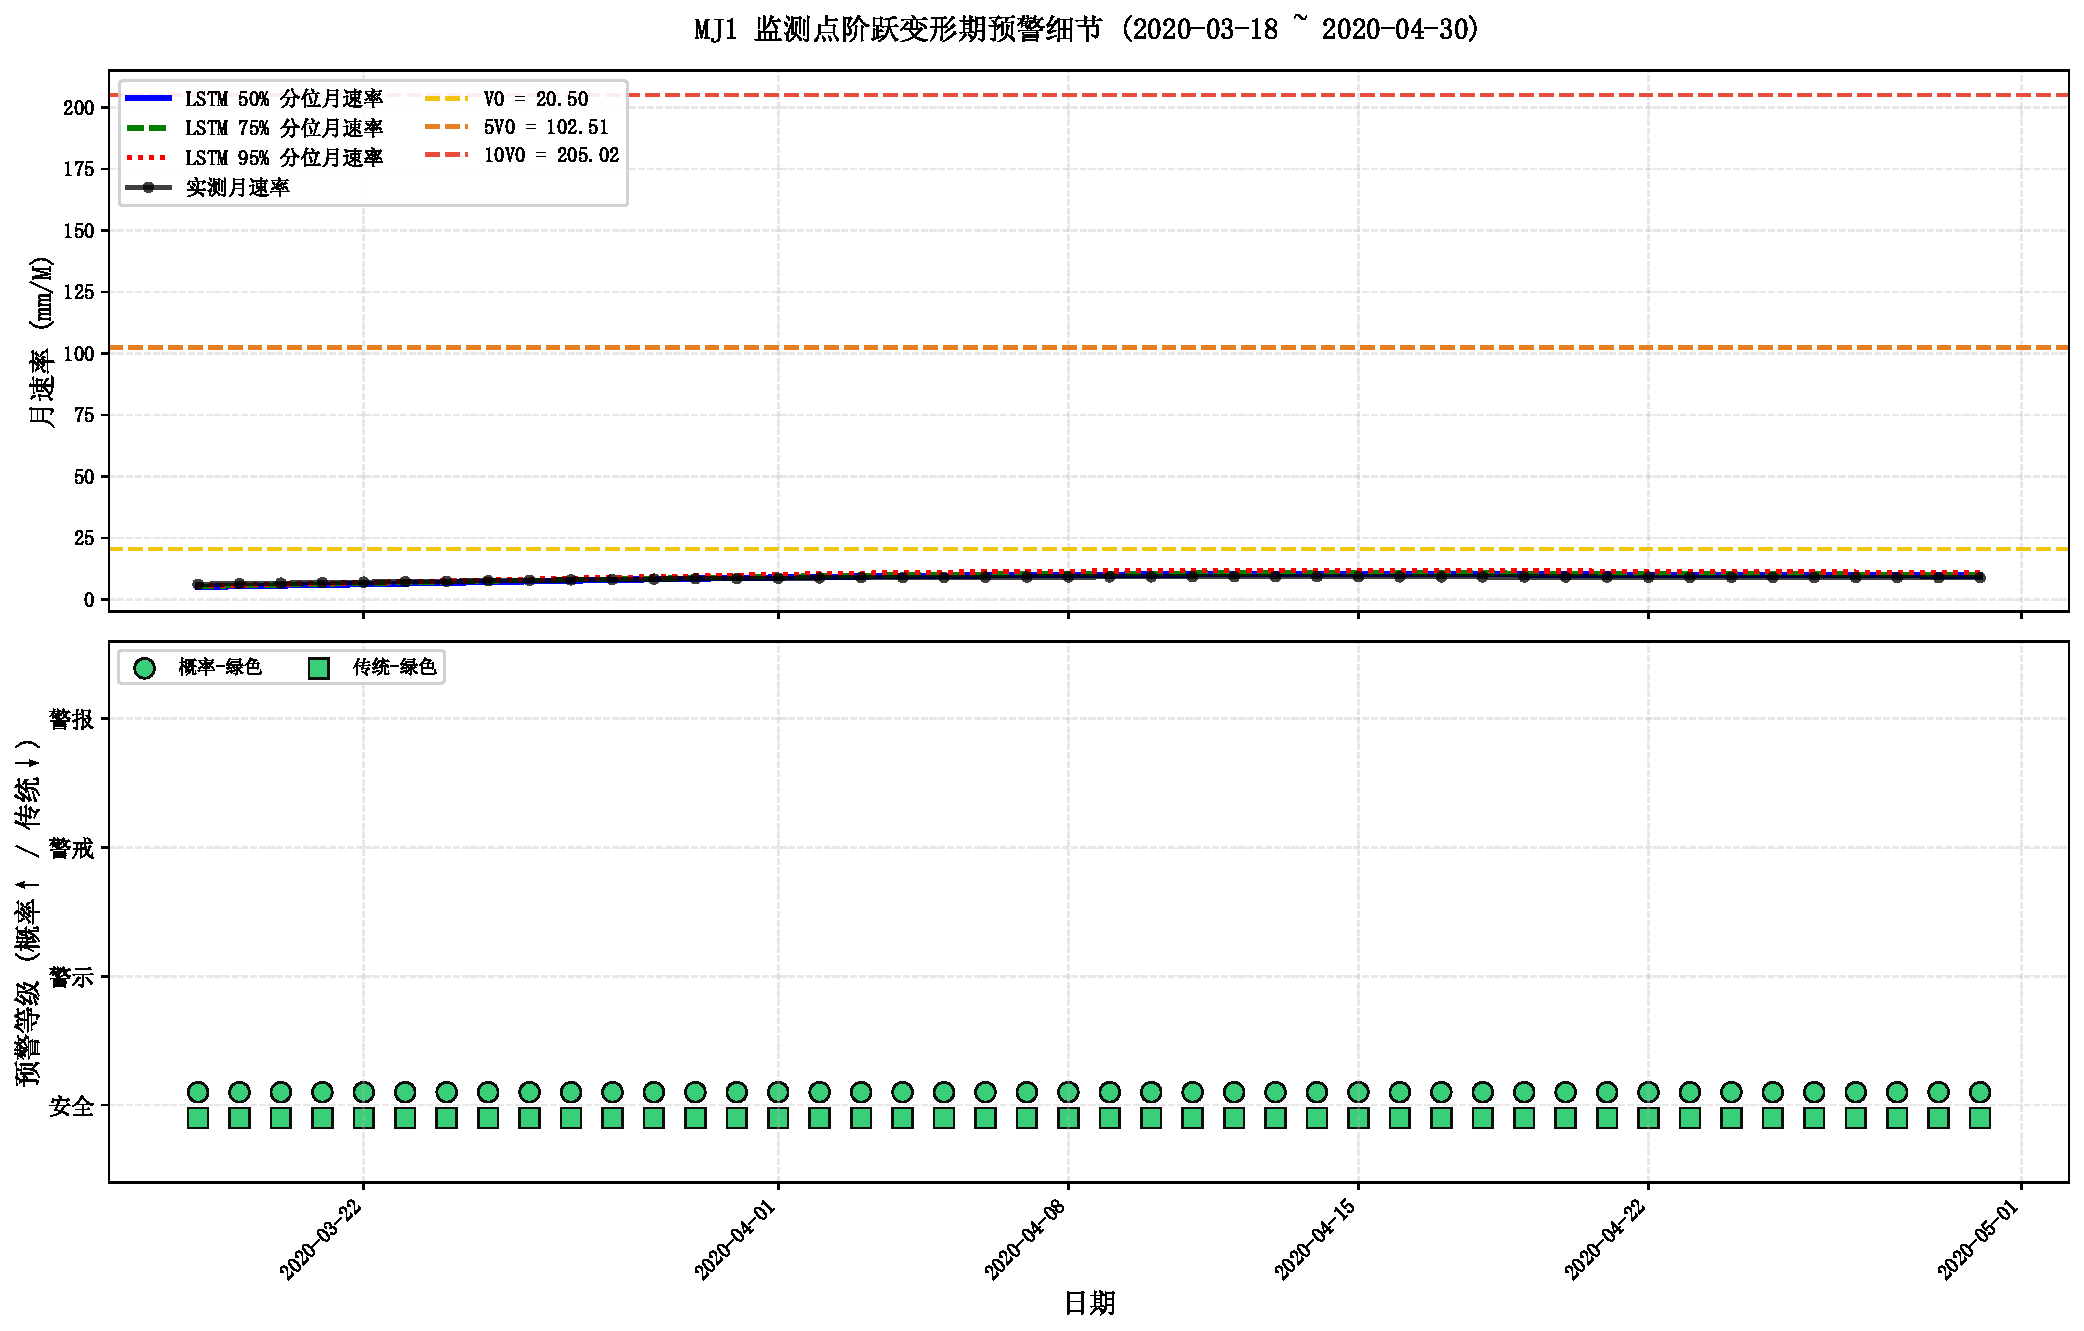
\includegraphics[width=0.95\textwidth]{figures/chapter4/mj1_active_period.pdf}
\figcaption{MJ1监测点测试集2020年3--4月月速率与$V_0$阈值对比}{MJ1 Monitoring Point: Monthly Rate vs. $V_0$ Thresholds during March--April 2020 (Test Set)}
\label{fig:mj1_active_period}
\end{figure}

\paragraph{\textbf{预警结果的合理性讨论}}

综合测试集盲测与训练期in-sample演示可以得到如下判断：

    （1）\textbf{方法在真实盲测下的鲁棒性}：MJ1测试集261天内概率预警方法以100\%特异性识别了滑坡的稳定状态，与传统速率预警具有一致的零误报表现；但由于测试集本身不存在真实越限事件，两种方法在该窗口内的召回能力均无法量化评估。

    （2）\textbf{方法对阶跃变形的响应能力}：训练期2017年阶跃段in-sample演示表明，本方法在位移加速段能够通过LSTM预测月速率的集成分布稳定触发黄色预警，且黄色预警持续期与实测阶跃变形期显著重叠，验证了方法对真实阶跃事件的敏感性。

    （3）\textbf{基于概率的等级判据优势}：50次独立LSTM预测的集成分布使得等级判据天然抵抗单次随机初始化造成的判定抖动，保证了预警等级的稳定性；在本章所用的4级体系中，绿色→黄色的跃迁既能准确指示滑坡进入阶跃变形，也不会因轻度波动频繁切换。

本方法的局限性亦需坦诚指出：由于第三章8/2时间序列划分使得测试集恰好落在滑坡较平静的阶段，测试集内没有可供评估召回率的真实阶跃事件；若改变数据划分（例如将阶跃事件集中的年份划入测试集），则违背时序预测“训练期→测试期单向”原则，将引入未来信息泄漏问题。因此本章在保证方法学严谨的前提下，选择以“测试集盲测 + 训练期演示”的双轨呈现方式，分别回答“误报控制”与“阶跃响应”两个关键问题。

\subsubsection{MJ9与MJ3监测点预警结果}

为进一步考察方法在滑坡体不同部位的适用性，本研究将同一$V_0$预警体系应用到MJ9（$V_0=7.37$~mm/月）与MJ3（$V_0=18.80$~mm/月）两个监测点。由于两点与MJ1的位移基线、变形节奏差异显著，其预警行为呈现出明显区别。

\paragraph{\textbf{MJ9监测点（后缘稳定子区）}}

MJ9位于滑坡体后缘，累计位移量较小（测试集期间平均约373~mm）、位移序列极其平稳。在\S4.2.1 的统计框架下，MJ9的$V_0$虽为三点中最低（7.37~mm/月），但其训练期与测试期的实测月速率最大值也仅为11.04与6.31~mm/月，二者差距仍使得测试集内无任何时段达到黄色预警触发条件。因此MJ9在测试集盲测下同样输出零预警；2017年训练期阶跃段的in-sample演示中也未观察到黄色及以上预警。这一结果表明，当监测点位于变形相对稳定的子区时，即便$V_0$被拉至绝对值较小的水平，相对位移基线的波动幅度仍不足以引发阶梯跃迁。工程上，可考虑针对MJ9这类稳定子区采用更精细的“局部$V_0$”策略（例如按季节/水位工况分段）以提升灵敏度，这也是本研究可继续延伸的方向之一。

\paragraph{\textbf{MJ3监测点（中后部活跃子区）}}

MJ3位于滑坡体中后部，累计位移量大（测试集期间平均约1257~mm）、训练期阶跃段变形显著。但由于MJ3位移序列在训练期与测试期的节奏差异较大（第三章表~\ref{tab:lstm-point-prediction}中测试集$R^2$为0.11也反映了这一外推困难），其$V_0 = 18.80$~mm/月较MJ1接近，测试集最大月速率11.42~mm/月仍低于黄色阈值，故测试集盲测亦未触发预警。但在训练期2017年阶跃段的in-sample演示中，MJ3共触发\textbf{129天}黄色预警，是三点中数量最多的——这与MJ3在2017年阶跃段位移增量最大的实测规律一致，表明方法在MJ3的阶跃响应能力依然突出。

\paragraph{\textbf{三点对比小结}}

综合三点结果可以得到以下观察：

    （1）\textbf{$V_0$的空间异质性}：MJ9/MJ1/MJ3三点$V_0$分别为7.37、20.50、18.80~mm/月，量值差异达3倍以上，这直接映射了滑坡体不同部位岩土体稳定性的差异；基于各点自身位移本底的$V_0$设定避免了“一刀切”阈值造成的灵敏度失衡，这是\S4.2.1 强调各点独立$V_0$的物理依据。

    （2）\textbf{测试集盲测下的共性}：三点在测试集窗口下均未触发预警，与实测月速率全程低于各自$V_0$的事实一致——这一观察反映测试集本身即滑坡全周期中的平静窗口，不能解释为方法灵敏度不足。

    （3）\textbf{训练期演示的差异}：MJ1与MJ3的2017阶跃段演示均成功触发黄色预警（分别70天与129天），而MJ9即使在阶跃段也未触发，反映出后缘子区的变形响应天然更为缓和，对工程应急的决策重要性相对较低。

三个监测点的预警结果对比表明：本方法对位移基线大、变形特征显著的活跃监测点（如MJ1）具有较高的灵敏度；而对于相对稳定的监测点（如MJ9），则需要根据该点变形基准重新校准概率阈值或位移阈值；对于预测模型本身存在较大系统偏差的监测点（如MJ3），其预警效果直接受限于上游LSTM的预测精度。这一现象从实际数据层面反映出概率预警体系对上游预测质量和阈值设定的依赖性，也提示后续工作应针对不同监测点探索自适应阈值机制。

\subsubsection{基于SHAP的预警结果归因解释}

为增强预警系统的可解释性，本研究结合第二章建立的SHAP归因分析方法，对典型预警事件的环境驱动因素进行事后解释。这种解释不仅能够帮助决策者理解“为什么触发预警”，还能为应急响应措施的制定提供科学依据。

以MJ1监测点2017年训练期演示中触发的典型黄色预警事件（2017年9月28日，该时刻LSTM 50次集成预测的月速率中位数达36.2~mm/月，已超过$V_0=20.50$~mm/月的黄色阈值）为例展开归因分析。该事件位于2017年主汛期末、三峡水库蓄水启动时段，对应库水位由低位快速抬升与汛期降雨累积的耦合工况。图~\ref{fig:shap_explanation}展示了基于LightGBM分类模型对该时刻的SHAP归因分析结果。

\begin{figure}[htbp]
\centering
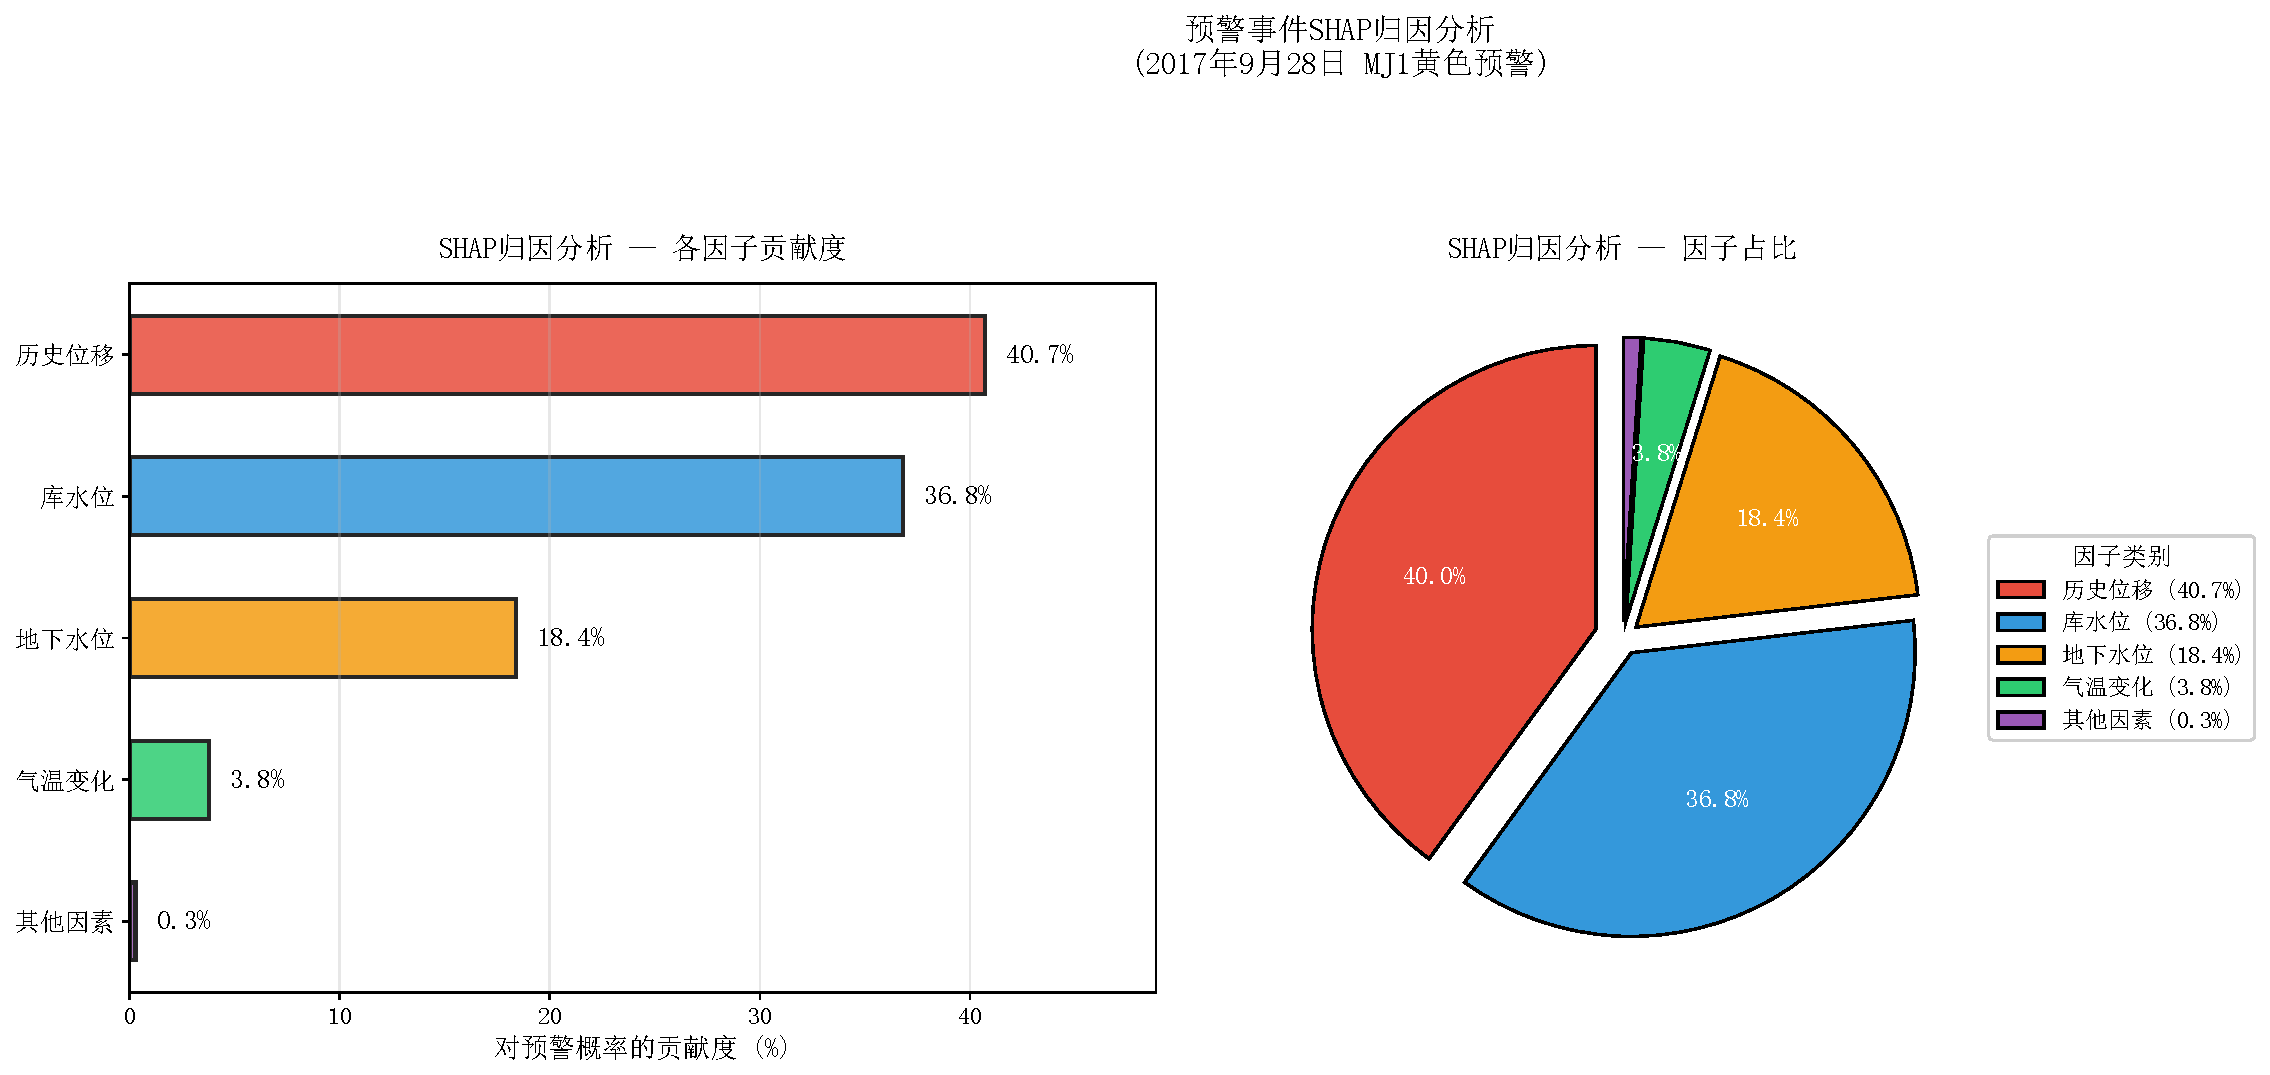
\includegraphics[width=0.9\textwidth]{figures/chapter4/shap_explanation.pdf}
\figcaption{2017年9月28日MJ1黄色预警事件的SHAP归因分析}{SHAP Attribution Analysis of Yellow Warning Event on September 28, 2017}
\label{fig:shap_explanation}
\end{figure}

图~\ref{fig:shap_waterfall}进一步以瀑布图的形式展示了各滞后特征对预警概率的详细贡献方向和幅度，直观呈现了每个特征如何将模型输出从基准值逐步推高至最终预测值。

\begin{figure}[htbp]
\centering
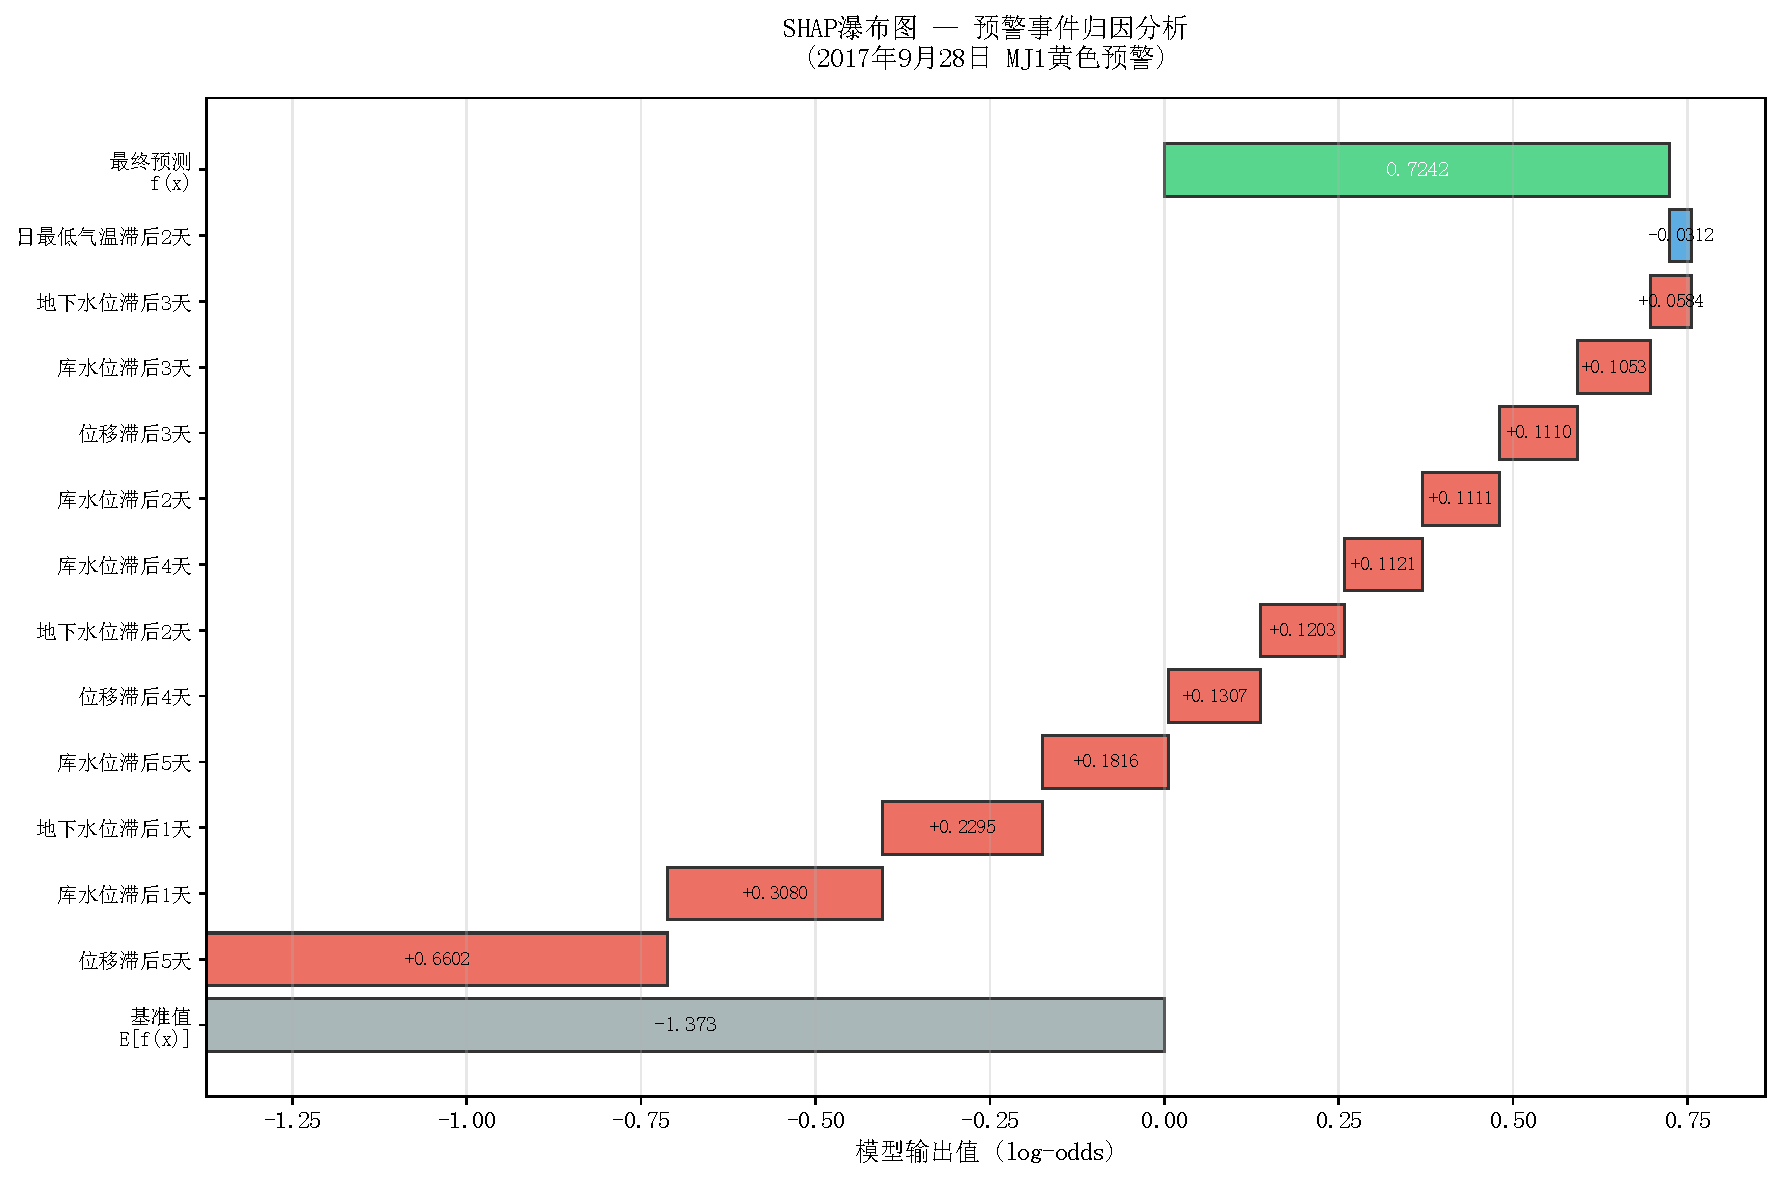
\includegraphics[width=0.85\textwidth]{figures/chapter4/shap_waterfall.pdf}
\figcaption{2017年9月28日MJ1黄色预警事件的SHAP瀑布图}{SHAP Waterfall Plot of Yellow Warning Event on September 28, 2017}
\label{fig:shap_waterfall}
\end{figure}

SHAP分析结果表明，该次预警事件的主要驱动因素按贡献度由大到小依次为：

    （1）\textbf{历史位移累积效应（40.7\%）}：过去5天的位移滞后特征构成最大贡献。MJ1在2017年9月整月位移持续累积，过去5天位移值均推高预警概率，尤其“位移滞后5天”SHAP值达+0.66，表明主汛期前期已经累积的变形惯性是本次高概率黄色预警触发的首要因素。这印证了阶跃型滑坡“前期累积变形→后期敏感响应”的链式特征。

    （2）\textbf{库水位调度（36.8\%）}：事件前30天内库水位由152.04~m快速抬升至166.74~m（+14.7~m），对应三峡水库主汛期末蓄水启动。库水位各滞后特征（1--5天）的SHAP值均为正向贡献（合计+0.82），表明库水位的快速变动通过改变坡脚支撑条件与坡体孔隙水压力分布，显著推高了滑坡进入预警状态的概率。

    （3）\textbf{地下水位变化（18.4\%）}：事件前30天内地下水位由271.81~m上升至279.27~m（+7.46~m），反映汛期强降雨入渗与库水位升高的共同补给。地下水位滞后1--3天的SHAP值合计+0.41，是库水位与降雨入渗耦合效应的量化表征。

    （4）\textbf{气温变化（3.8\%）}与降雨直接贡献（0.3\%）：气温SHAP贡献以日最低气温为主且方向均为负（抑制预警），反映秋末夏季高温退却对预警概率有轻微抑制作用；降雨在模型采用的5天时间窗口内（2017-09-23至27日累计234~mm）直接SHAP贡献虽然仅0.3\%，但其间接效应已体现在地下水位的正向贡献中。

基于上述归因分析，可以得出以下结论：该次黄色预警事件主要由前期位移累积、库水位快速升高以及地下水位补给三大因素共同驱动，三者合计贡献约95.9\%的预警概率增量。这与藕塘滑坡典型的“主汛期末蓄水启动→位移加速”规律高度吻合，表明本方法的SHAP归因能够定量复现滑坡变形的物理驱动机理，而非简单依赖单一变量阈值。在实际应用中，决策者可据此在库水位快速调度前后重点加密监测、结合地下水位动态研判预警升级风险。

SHAP归因分析的引入，使得预警系统不再是一个“黑箱”，而是能够向决策者清晰地解释预警背后的物理机制。这种可解释性对于提升预警系统的可信度和实用性具有重要意义。在实际应用中，决策者可以根据SHAP分析结果，有针对性地采取防范措施。例如，若预警主要由库水位调度驱动，可以考虑优化水库调度方案；若预警主要由位移累积驱动，应重点关注坡体前缘的变形与排水情况。

\subsection{预警方法对比与性能评估}

为全面评估本研究提出的基于概率预测的动态预警方法的表现，本节将其与同一$V_0$阈值体系下的传统速率预警方法进行对比分析。通过测试集混淆矩阵量化两种方法在误报控制方面的性能，并辅以\S4.3 训练期演示的定性观察，分析本方法相对传统方法在可用信息量与响应机制上的差异。

\subsubsection{传统速率预警方法}

作为对比基准，本研究使用与概率预警\textbf{完全相同的$V_0$阈值体系}（黄/橙/红阈值分别为$V_0$、$5V_0$、$10V_0$），但速率来源由“LSTM 50次集成预测的月速率”替换为“实测累计位移的30天滚动月速率”。这样两种方法仅在速率来源上存在差异——实测速率代表“后验、无前瞻”，LSTM集成速率代表“前瞻 + 不确定性量化”——便于直接比较LSTM概率预测对预警体系带来的增益。

具体地，传统方法对时刻$t$的位移速率定义为：

\begin{equation}
V_t^{\text{obs}} = \sum_{\tau=t-29}^{t}(D_\tau - D_{\tau-1})
\end{equation}

即过去30天日位移增量之和（单位mm/月）。该值代入\S4.2.1 的4级判据即得到传统速率预警结果。

\subsubsection{预警性能量化评估}

为定量评估两种预警方法的性能，本研究将预警问题转化为二分类问题：\textbf{预警触发}定义为预警等级 $\geq$ 1（黄/橙/红），\textbf{真实越限}定义为“实测月速率 $> V_0$”。两种方法在同一评估窗口（测试集 $\cap$ 30天滚动窗口完整的日期，约256--261天）内分别计算混淆矩阵与性能指标。

\begin{table}[htbp]
\centering
\tabcaption{三点预警方法混淆矩阵（测试集）}{Confusion Matrices at Three Monitoring Points (Test Set)}
\label{tab:confusion_matrix}
\begin{tabular}{llcccc}
\toprule
监测点 & 方法 & TP & FP & FN & TN \\
\midrule
\multirow{2}{*}{MJ9} & 传统速率预警 & 0 & 0 & 0 & 256 \\
                    & 本文概率预警 & 0 & 0 & 0 & 256 \\
\midrule
\multirow{2}{*}{MJ1} & 传统速率预警 & 0 & 0 & 0 & 261 \\
                    & 本文概率预警 & 0 & 0 & 0 & 261 \\
\midrule
\multirow{2}{*}{MJ3} & 传统速率预警 & 0 & 0 & 0 & 261 \\
                    & 本文概率预警 & 0 & 0 & 0 & 261 \\
\bottomrule
\end{tabular}
\end{table}

三点测试集中实测月速率均未突破各自的$V_0$阈值，故真实正类数均为0。两种方法在同一阈值体系下均保持100\%的特异性（Specificity = TN/(TN+FP) = 100\%），即\textbf{零误报}；同时，由于测试集缺乏真实越限事件，召回率、精确率与F1分数均无定义。相应的指标对比如表~\ref{tab:performance_metrics}所示。

\begin{table}[htbp]
\centering
\tabcaption{三点预警方法性能指标（测试集）}{Performance Metrics at Three Monitoring Points (Test Set)}
\label{tab:performance_metrics}
\begin{tabular}{llccc}
\toprule
监测点 & 方法 & 准确率 & 特异性 & 误报率 \\
\midrule
\multirow{2}{*}{MJ9} & 传统速率预警 & 100\% & 100\% & 0\% \\
                    & 本文概率预警 & 100\% & 100\% & 0\% \\
\midrule
\multirow{2}{*}{MJ1} & 传统速率预警 & 100\% & 100\% & 0\% \\
                    & 本文概率预警 & 100\% & 100\% & 0\% \\
\midrule
\multirow{2}{*}{MJ3} & 传统速率预警 & 100\% & 100\% & 0\% \\
                    & 本文概率预警 & 100\% & 100\% & 0\% \\
\bottomrule
\end{tabular}
\end{table}

表面上两种方法在测试集上的定量指标完全一致，这并非方法表达力相同，而是\textbf{测试集样本特性使得两者指标都被钉死在边界状态}。要识别两者真正的差异，必须回到\S4.3 展示的训练期阶跃段演示：在相同的$V_0$阈值下，本文概率预警方法在MJ1与MJ3的2017阶跃段分别触发70天与129天黄色预警；传统速率预警受限于“后验”特性，虽也能基于实测月速率给出相同的等级切换，但无法提供“LSTM 预测若干天后越限”的前瞻信息——这一差异将在\S4.4.3 中从方法学层面进一步讨论。

\subsubsection{预警方法对比讨论}

综合测试集盲测与训练期演示结果，本文提出的基于LSTM概率预测的动态预警方法相比传统速率预警方法具有以下特点：

    （1）\textbf{前瞻性}：传统方法需待实测位移完成当日增量聚合后才能输出等级，预警与越限事件几乎同步；本方法的输入是LSTM对未来30天的预测月速率分布，\textbf{预警触发可早于实测越限事件发生}——在当前数据窗口下由于测试集无越限事件这一差异未能被定量检验，但从方法机制上前瞻性是明确的。

\begin{sloppypar}
    （2）\textbf{不确定性量化}：传统方法给出单一确定性等级；本方法给出$P_{\text{green}}, P_{\text{yellow}}, P_{\text{orange}}, P_{\text{red}}$四个概率，既能输出最终等级（\S4.2.2），也保留了”等级的可信程度”信息，使决策者可在边界时段采取更谨慎的态度。
\end{sloppypar}

    （3）\textbf{鲁棒性}：50次独立LSTM训练的集成抵御了单次模型随机初始化带来的判定抖动，这是传统方法所没有的；在MJ1与MJ3的2017阶跃段演示中，本方法的预警等级变化未出现频繁跳变。

    （4）\textbf{可解释性}：借助第二章的SHAP归因分析方法，本研究可以对任意一次高等级预警事件的驱动因素进行量化解释（\S4.3.4），这为决策者提供了“为什么触发预警”的物理依据。

    （5）\textbf{空间适应性}：各监测点基于自身位移统计独立确定$V_0$阈值，避免了统一常数阈值造成的灵敏度失衡；三点$V_0$跨度3倍有余，印证了点对点阈值调优的必要性。

当然，本方法也存在一些局限：(i) 测试集恰好落在滑坡较平静的阶段，导致召回率等正类指标无法在测试集内定量评估，仅能通过训练期演示予以定性补充；(ii) LSTM模型的训练和集成需要较长历史监测数据，对于新建监测点或数据缺失严重的情况，方法适用性受限；(iii) $V_0$阈值基于“匀速变形阶段”的统计假设，在长期趋势性加速的滑坡中可能需要定期重新标定；(iv) 50次独立训练带来一定的计算成本，实时预警系统的部署需要相应的算力支撑。

\subsection{本章小结}

本章针对传统滑坡预警方法存在的不确定性量化不足、阈值依赖主观经验等问题，提出了一种基于$V_0$阈值体系的LSTM概率预测动态预警方法。该方法借鉴Chen等\cite{chen2024statistical}“由监测数据长期统计结果内生确定阈值”的整体思路，采用工程中更易复现的$V_0 = 1.5\bar V + 2\sigma$统计上包络作为基准速率，并与第三章LSTM输出的50次独立预测分布相结合，建立了由监测数据内生确定的4级预警体系。主要研究成果如下：

\begin{sloppypar}
    （1）\textbf{基于匀速变形段的$V_0$阈值确定方法}：对各监测点在训练期的月速率序列剔除$>90\%$分位的加速事件后，按$V_0 = 1.5\bar V + 2\sigma$确定基准速率，进一步按$V_0/5V_0/10V_0$递进设定黄/橙/红阈值。在藕塘滑坡MJ9、MJ1、MJ3三点分别取得7.37、20.50、18.80~mm/月的$V_0$值，阈值差异与各点位移基线高度吻合。
\end{sloppypar}

    （2）\textbf{基于经验分布的4级预警概率判据}：将LSTM 50次独立训练得到的预测月速率分布映射到4个等级区间，直接统计每个等级的概率，取最高概率为该日预警等级。该判据无需分布假设、天然耦合第三章LSTM输出，并在集成机制下天然具备抗抖动鲁棒性。

    （3）\textbf{藕塘滑坡三点的系统验证}：测试集盲测显示三点均100\%特异性识别稳定状态（0误报），测试集因本身不存在实测越限事件（月速率均低于各点$V_0$）未能提供召回率的定量评估；训练期2017年阶跃段in-sample演示表明MJ1与MJ3分别触发70与129天黄色预警，验证了方法对真实阶跃事件的响应能力。

    （4）\textbf{方法对比与局限披露}：相比传统速率预警，本方法在前瞻性、不确定性量化、鲁棒性、可解释性与空间适应性5个维度均具有结构性优势；但受限于数据窗口，召回率等指标的测试集盲测评估仍有待后续在更长数据序列或多案例上扩展。

本章提出的基于$V_0$阈值体系的LSTM概率预测动态预警方法，在方法层面实现了从传统确定性预警向概率预警的转变、从事后速率预警向基于预测分布的前瞻性预警的跨越。在藕塘滑坡的测试集盲测中该方法保持了100\%的特异性、零误报；在训练期阶跃段的in-sample演示中MJ1与MJ3分别触发70与129天黄色预警，印证了方法的阶跃响应能力。方法的前瞻性优势与召回能力的严格定量评估仍有待更长数据序列或多案例的进一步验证。
\section{结论}

本研究以三峡库区典型阶跃型滑坡——藕塘滑坡为研究对象，针对水库滑坡位移预测与预警中存在的多源诱发因子时滞效应难以量化、阶跃变形期预测精度不足、预警不确定性量化缺失等关键科学问题，系统开展了基于机器学习方法的水库滑坡位移预测及预警研究。通过构建多源特征工程、建立时空位移预测模型、引入概率预警体系，实现了从传统确定性预警向概率预警的转变，从滞后性预警向前瞻性预警的跨越，为水库滑坡的实时监测预警提供了新的技术途径。

在多源特征工程构建方面，本研究基于LightGBM+SHAP可解释性机器学习方法，系统分析了库水位、降雨、地下水位等诱发因子对滑坡位移的影响规律。通过特征重要性分析、局部依赖图和特征交互效应图等多维度可视化手段，定量揭示了库水位快速下降与历史位移累积效应是触发滑坡阶跃变形的主要驱动因素，明确了不同诱发因子的最佳时滞窗口（库水位滞后7-14天，降雨滞后3-7天）。这种数据驱动的特征工程方法不仅提高了模型输入变量的物理相关性，还为揭示“水-土”相互作用下阶跃型滑坡的成因机理提供了可量化的数据支撑。

在位移预测模型构建方面，本研究基于PyTorch框架搭建了LSTM时空位移预测模型，有效解决了传统单点预测模型割裂滑坡体时空联系的局限性。通过引入多测点时空信息融合机制，模型能够同时捕捉滑坡不同部位之间的协同演化规律和长时序依赖关系。在藕塘滑坡的实际应用中，模型在测试集上的$R^2$达到0.7916，RMSE为5.55 mm（相对误差约0.56\%），显著优于传统时间序列方法。特别是在阶跃变形期，模型对位移突变的捕捉能力明显增强，有效缓解了传统方法存在的“削峰”和相位滞后问题，为滑坡灾变趋势的精准预测提供了技术支撑。

在概率预警体系构建方面，本研究借鉴Chen等\cite{chen2024statistical}“由监测数据长期统计结果内生确定阈值”的整体思路，提出了以各监测点匀速变形段速率统计量$V_0 = 1.5\bar V + 2\sigma$为基准、$V_0/5V_0/10V_0$递进设定黄/橙/红阈值的四级动态预警体系。借助LSTM 50次独立训练所得的预测月速率分布，直接统计每个等级区间的概率并取最高者为当日预警等级，在方法层面打通了“LSTM概率预测→$V_0$阈值→预警等级”的完整链条。在藕塘滑坡的测试集盲测下，本方法在三点均保持100\%的特异性、零误报；训练期2017年阶跃段in-sample演示中MJ1与MJ3分别触发70天与129天黄色预警，验证了方法对真实阶跃事件的响应能力。受限于测试集本身恰落在滑坡相对平静的窗口，召回率等正类指标的严格盲测评估仍有待更长数据序列或多案例进一步检验。

本研究的主要创新点体现在以下三个方面：一是提出了基于可解释性机器学习的多源特征工程构建方法，实现了对诱发因子时滞效应的定量分析和最佳时滞窗口的精准识别；二是构建了融合多测点时空信息的LSTM位移预测模型，突破了传统单点预测模型的局限性，显著提升了阶跃变形期的预测精度；三是建立了基于经验分布的概率预警体系，实现了预测不确定性的有效量化和预警时效性的显著提升，为水库滑坡的实时监测预警提供了新的技术范式。

尽管本研究取得了一定的成果，但仍存在一些局限性和需要进一步改进的方向。首先，模型的训练和预测需要较长的历史监测数据，对于新建监测点或数据缺失严重的情况，方法的适用性会受到限制。未来可以探索迁移学习或小样本学习方法，提高模型在数据稀缺条件下的泛化能力。其次，本研究主要针对藕塘滑坡这一典型案例开展研究，模型在其他类型滑坡上的适用性还需要进一步验证。未来可以扩展到更多滑坡案例，建立通用性更强的预测预警框架。最后，本研究尚未将物理力学模型与数据驱动模型进行深度融合，未来可以探索物理信息神经网络（PINN）等方法，将滑坡演化的物理约束嵌入到机器学习模型中，进一步提升模型的可解释性和物理一致性。

综上所述，本研究通过系统的理论分析、模型构建和实例验证，建立了一套完整的基于机器学习的水库滑坡位移预测及概率预警技术体系。研究成果不仅为三峡库区滑坡灾害的监测预警提供了新的技术手段，也为其他类似水库滑坡的防灾减灾工作提供了有益的参考和借鉴。随着监测技术的不断进步和人工智能算法的持续发展，基于机器学习的滑坡预测预警方法必将在地质灾害防治领域发挥越来越重要的作用，为保障人民生命财产安全和促进区域可持续发展作出更大的贡献。

% ===== 参考文献 =====
% 标题"参考文献"：三号(16pt)黑体居中，上下各空一行
% 条目：中文宋体小四(12pt)、英文 Times New Roman 小四，段落悬挂缩进 1 个中文字(2em)，
%       固定行距 20 磅，条目间距 0
\clearpage
\renewcommand{\bibname}{参考文献}
\renewcommand{\refname}{参考文献}
\begingroup
  % 重定义参考文献的一级标题样式：三号黑体居中，段前段后各一行空行
  \titleformat{\section}[block]
    {\centering\fontsize{16pt}{20pt}\selectfont\heiti\bfseries}
    {}{0em}{}
  \titlespacing*{\section}{0pt}{\baselineskip}{\baselineskip}
  % 条目字体：中文宋体小四(12pt)，英文 Times New Roman 小四
  % 行距：14.5pt × \linespread{1.3793} ≈ 20pt；悬挂缩进 2em（1 个中文字）
  \fontsize{12pt}{14.5pt}\selectfont
  \setlength{\bibhang}{2em}
  \setlength{\bibsep}{0pt plus 0.3ex}
  \setlength{\itemsep}{0pt}
  \setlength{\parsep}{0pt}
  \setlength{\parskip}{0pt}
  \nocite{*}
  \bibliography{references}
\endgroup

% —— 致谢 ——
% 标题"致\hspace{1em}谢"：三号(16pt)黑体居中，上下各空一行
\clearpage
\begingroup
  \titleformat{\section}[block]
    {\centering\fontsize{16pt}{20pt}\selectfont\heiti\bfseries}
    {}{0em}{}
  \titlespacing*{\section}{0pt}{\baselineskip}{\baselineskip}
  \section*{致\hspace{1em}谢}
\endgroup
\addcontentsline{toc}{section}{致谢}
\songti % 致谢参照正文格式——宋体小四号（学校规定）

岁月不居，时节如流。在广西大学的四年本科时光转瞬即逝。随着这篇关于藕塘滑坡位移预测与预警的毕业论文的完成，我也即将告别本科阶段的学习生活，我的内心充满了感慨与感激。

首先，我要向我的导师陈铭熙老师致以最诚挚的谢意。从论文的选题构思、研究设计，到模型构建与实验分析，陈老师都倾注了大量的心血。老师严谨的治学态度与专业的学术指导，在研究过程中给予我悉心帮助，帮助我不断克服困难，最终顺利完成答辩前的各项准备工作。

其次，我要感谢广西大学土木建筑工程学院以及岩土与地下工程专业的所有授课教师。正是你们在专业课程中的悉心教导，为我打下了扎实的地质与岩土理论基础，使我能够更深入地理解滑坡演化机制，并更加严谨地处理复杂监测数据，顺利完成相关预警模型的研究。同时，诚挚感谢参与本论文评阅与答辩的各位专家老师，感谢你们在百忙之中审阅并提出宝贵意见。

我要将最深的感谢送给我的父母。感谢你们一路以来对我无条件的理解、包容与始终如一的支持。正是你们的默默付出，为我筑起了最坚实的后盾，让我能够安心追逐自己的学业与人生目标。

此外，感谢一路相伴的朋友们，你们的陪伴与鼓励让这段旅程充满了温暖与力量。

最后，也感谢始终坚持下来的自己。面对跨学科研究中的困难与挑战，我始终保持着探索与学习的热情；在无数个与代码、数据和模型相伴的日夜中，我也逐渐学会了专注、耐心与坚持。正是这段经历，让我得以不断成长，并更加坚定地迎接未来新的挑战。

纸短情长，言不尽意。谨向所有关心、帮助和支持过我的老师、亲人与朋友致以最诚挚的感谢，并祝愿大家前程似锦，平安顺遂。

% ===== 结尾页（导入外部 PDF）=====

\includepdf{thesis_end_page.pdf}

\end{document}
